\documentclass{book}

\usepackage[a4paper,margin=3cm]{geometry}
\usepackage{cite} % for IEEE-style citations
\usepackage{listings}
\usepackage{xcolor}
\usepackage[hidelinks]{hyperref}
\usepackage{graphicx}
\usepackage{setspace}
\usepackage{tcolorbox}
\usepackage{tikz}
\usetikzlibrary{trees}

\renewcommand{\contentsname}{Daftar Isi}
\renewcommand{\chaptername}{Bab}

% Define Java language style for listings
\lstdefinestyle{JavaStyle}{
	language=Java,
	basicstyle=\ttfamily\footnotesize,
	keywordstyle=\color{blue},
	commentstyle=\color{gray},
	stringstyle=\color{red},
	breaklines=true,
	showstringspaces=false,
	tabsize=2,
	captionpos=b,
	numbers=left,
	numberstyle=\tiny\color{gray},
	frame=lines,
	backgroundcolor=\color{lightgray!10},
	comment=[l]{//},
	morecomment=[s]{/*}{*/},
	commentstyle=\color{gray}\ttfamily,
	string=[s]{'}{'},
	morestring=[s]{"}{"},
	%	stringstyle=\color{teal}\ttfamily,
	%	showstringspaces=false
}


\begin{document}
		
	\begin{titlepage}
		\centering
		\vspace*{1cm}
		
		\Huge
		\textbf{IF120203 - Modul Praktikum Pemrograman Dasar}
		
		\vspace{0.5cm}
		
		\LARGE
		Universitas Pradita
		
		\vspace{1.5cm}
		
		\textit{Powered by ChatGPT}
		
		\vspace{2cm}
		
		\textbf{Alfa Yohannis, Patricia Ho}
		
		\vspace{0.8cm}
		
		\today
		
		\vfill
	\end{titlepage}
	
	% Contents Page
	\tableofcontents
	
	
	
\chapter{Pendahuluan}

\section{Sejarah Pemrograman dan Java}

Pemrograman komputer dimulai pada abad ke-19 dengan penemuan mesin analitik oleh Charles Babbage dan program pertama yang ditulis oleh Ada Lovelace. Sejak itu, pemrograman telah berkembang pesat dengan munculnya bahasa-bahasa pemrograman awal seperti Fortran, COBOL, dan Lisp pada tahun 1950-an. Pada tahun 1970-an dan 1980-an, bahasa pemrograman seperti C, Pascal, dan Basic memperkenalkan konsep-konsep baru dalam pemrograman. Kini, berbagai bahasa pemrograman modern seperti Python, JavaScript, dan Rust digunakan dalam berbagai aplikasi.

Java adalah bahasa pemrograman yang dikembangkan oleh Sun Microsystems pada tahun 1995. Java dirancang dengan prinsip "Write Once, Run Anywhere" yang memungkinkan program Java untuk berjalan di berbagai platform tanpa perlu diubah. Java terkenal karena kemampuannya dalam pengembangan aplikasi web, aplikasi mobile, dan aplikasi desktop. Versi terbaru dari Java terus dikembangkan untuk memperkenalkan fitur-fitur baru dan meningkatkan kinerja.

\section{Instalasi di Windows}

Untuk menginstal Java di Windows, ikuti langkah-langkah berikut:

\begin{enumerate}
\item Unduh installer JDK terbaru dari situs resmi Oracle atau OpenJDK.
\item Jalankan file installer dan ikuti petunjuk untuk menyelesaikan instalasi.
\item Tambahkan direktori `bin` dari JDK ke variabel lingkungan `PATH`. Anda dapat melakukannya melalui Control Panel > System > Advanced system settings > Environment Variables.
\item Verifikasi instalasi dengan membuka Command Prompt dan mengetik `java -version` dan `javac -version`.
\end{enumerate}

\section{Instalasi di macOS}

Untuk menginstal Java di macOS, ikuti langkah-langkah berikut:

\begin{enumerate}
\item Unduh installer JDK terbaru dari situs resmi Oracle atau OpenJDK.
\item Jalankan file installer `.dmg` dan ikuti petunjuk untuk menyelesaikan instalasi.
\item Setelah instalasi selesai, verifikasi instalasi dengan membuka Terminal dan mengetik `java -version` dan `javac -version`.
\end{enumerate}

\section{Instalasi di Linux}

Untuk menginstal Java di Linux, ikuti langkah-langkah berikut:

\begin{enumerate}
\item Buka terminal dan jalankan perintah berikut untuk menginstal JDK:
\begin{verbatim}
	sudo apt update
	sudo apt install default-jdk
\end{verbatim}
\item Verifikasi instalasi dengan mengetik `java -version` dan `javac -version` di terminal.
\end{enumerate}

\section{IDE dan Penggunaan Eclipse}

\subsection{Apa Itu IDE?}

Integrated Development Environment (IDE) adalah perangkat lunak yang menyediakan fasilitas lengkap untuk pengembangan perangkat lunak. IDE umumnya mencakup editor kode, kompiler atau interpreter, debugger, dan alat manajemen proyek. IDE dirancang untuk mempermudah proses pengembangan perangkat lunak dengan menyediakan antarmuka pengguna yang terintegrasi dan alat-alat yang mendukung pengkodean, pengujian, dan debugging.

\subsection{Cara Menginstal Eclipse}

Untuk menginstal Eclipse, ikuti langkah-langkah berikut:

\begin{enumerate}
	\item Unduh installer Eclipse dari situs resminya \url{https://www.eclipse.org/downloads/}.
	\item Pilih versi Eclipse yang sesuai dengan kebutuhan Anda, seperti Eclipse IDE for Java Developers.
	\item Jalankan file installer yang telah diunduh.
	\item Pilih direktori instalasi dan klik `Install`.
	\item Setelah instalasi selesai, buka Eclipse dari direktori instalasi.
\end{enumerate}

\subsection{Cara Membuat Proyek Java Baru di Eclipse}

Untuk membuat proyek Java baru di Eclipse, ikuti langkah-langkah berikut:

\begin{enumerate}
	\item Buka Eclipse dan pilih workspace tempat Anda ingin menyimpan proyek.
	\item Pilih menu `File` > `New` > `Java Project`.
	\item Masukkan nama proyek di kotak `Project Name`.
	\item Klik `Finish` untuk membuat proyek baru.
	\item Untuk menambahkan file Java, klik kanan pada folder `src` di proyek Anda, pilih `New` > `Class`, masukkan nama kelas, dan klik `Finish`.
	\item Mulai menulis kode Java di editor yang muncul.
\end{enumerate}

\section{Kode Java: HelloWorld.java}

\begin{lstlisting}[style=JavaStyle, caption={Kode Java: HelloWorld.java}]
package hello;

public class HelloWorld {
	public static void main(String[] args) {
		System.out.println("Hello World!");
	}
}
\end{lstlisting}

Kode di atas merupakan program Java sederhana yang mencetak "Hello World!" ke konsol. Berikut penjelasan dari setiap bagian kode tersebut:

\begin{itemize}
\item \texttt{package hello;} - Mendeklarasikan bahwa kelas ini berada dalam paket \texttt{hello}. Paket membantu dalam mengelompokkan kelas yang berhubungan.
\item \texttt{public class HelloWorld \{\}} - Mendefinisikan kelas publik \texttt{HelloWorld}. Kelas adalah template atau blueprint dari objek.
\item \texttt{public static void main(String[] args) \{\}} - Fungsi utama (\texttt{main}) yang akan dijalankan pertama kali ketika program dieksekusi. Kata kunci \texttt{public} membuatnya dapat diakses dari luar, \texttt{static} membuatnya dapat dipanggil tanpa harus membuat objek, \texttt{void} menunjukkan bahwa fungsi ini tidak mengembalikan nilai, dan \texttt{String[] args} adalah parameter untuk mengambil argumen dari command line.
\item \texttt{System.out.println("Hello World!");} - Perintah ini mencetak teks "Hello World!" ke konsol. \texttt{System.out} adalah objek output standar, dan \texttt{println} adalah metode untuk mencetak dengan baris baru.
\end{itemize}

\section{Panduan Kompilasi dan Menjalankan Program}

Untuk mengkompilasi dan menjalankan program Java di atas, ikuti langkah-langkah berikut:

\begin{enumerate}
\item \textbf{Kompilasi Program:}
\begin{itemize}
	\item Buka terminal atau command prompt.
	\item Navigasikan ke direktori tempat file `HelloWorld.java` disimpan.
	\item Jalankan perintah berikut untuk mengkompilasi program:
	\begin{verbatim}
		javac HelloWorld.java
	\end{verbatim}
	\item Jika tidak ada error, file bytecode bernama `HelloWorld.class` akan dihasilkan.
\end{itemize}

\item \textbf{Menjalankan Program:}
\begin{itemize}
	\item Setelah kompilasi berhasil, jalankan program dengan perintah berikut:
	\begin{verbatim}
		java hello.HelloWorld
	\end{verbatim}
	\item Output "Hello World!" akan muncul di konsol.
\end{itemize}
\end{enumerate}

\section{Kode Java: HelloWorldWithInput.java}

\begin{lstlisting}[style=JavaStyle, caption={Kode Java: HelloWorldWithInput.java}]
package hello;

import java.util.Scanner;  // Import kelas Scanner

public class HelloWorldWithInput {
	public static void main(String[] args) {
		Scanner scanner = new Scanner(System.in);  // Membuat objek Scanner
		
		System.out.print("Masukkan nama Anda: ");
		String name = scanner.nextLine();  // Menerima input dari pengguna
		
		System.out.println("Hello " + name + "!");  // Menampilkan output dengan input pengguna
		
		scanner.close();  // Menutup Scanner untuk menghindari kebocoran sumber daya
	}
}
\end{lstlisting}

Kode di atas merupakan program Java yang meminta input nama dari pengguna dan mencetak pesan "Hello [Nama]!" ke konsol. Berikut penjelasan dari setiap bagian kode tersebut:

\begin{itemize}
\item \texttt{import java.util.Scanner;} - Mengimpor kelas \texttt{Scanner} dari paket \texttt{java.util} untuk membaca input dari pengguna.
\item \texttt{Scanner scanner = new Scanner(System.in);} - Membuat objek \texttt{Scanner} yang akan digunakan untuk membaca input dari konsol.
\item \texttt{String name = scanner.nextLine();} - Menerima input nama dari pengguna dan menyimpannya dalam variabel \texttt{name}.
\item \texttt{System.out.println("Hello " + name + "!");} - Mencetak pesan "Hello [Nama]!" ke konsol, di mana \texttt{name} adalah input dari pengguna.
\item \texttt{scanner.close();} - Menutup objek \texttt{Scanner} setelah digunakan untuk menghindari kebocoran sumber daya.
\end{itemize}


\section{Latihan}

Berikut adalah beberapa latihan yang dapat Anda coba untuk memperdalam pemahaman tentang program Java yang telah dibahas:

\begin{enumerate}
\item \textbf{Latihan 1:} Modifikasi kode \texttt{HelloWorld.java} untuk mencetak "Hello, [Nama Anda]!" menggunakan argumen command line. Program harus menerima nama dari argumen dan menampilkannya.

\begin{lstlisting}[style=JavaStyle, caption={Latihan 1}]
	package hello;
	
	public class HelloWorldWithArgs {
		public static void main(String[] args) {
			if (args.length > 0) {
				System.out.println("Hello, " + args[0] + "!");
			} else {
				System.out.println("Hello World!");
			}
		}
	}
\end{lstlisting}

\item \textbf{Latihan 2:} Tambahkan validasi input pada kode \texttt{HelloWorldWithInput.java} untuk memastikan bahwa nama yang dimasukkan tidak kosong. Jika nama kosong, program harus meminta input ulang.

\begin{lstlisting}[style=JavaStyle, caption={Latihan 2}]
	package hello;
	
	import java.util.Scanner;
	
	public class HelloWorldWithValidatedInput {
		public static void main(String[] args) {
			Scanner scanner = new Scanner(System.in);
			String name = "";
			
			while (name.isEmpty()) {
				System.out.print("Masukkan nama Anda: ");
				name = scanner.nextLine();
				
				if (name.isEmpty()) {
					System.out.println("Nama tidak boleh kosong. Silakan coba lagi.");
				}
			}
			
			System.out.println("Hello " + name + "!");
			scanner.close();
		}
	}
\end{lstlisting}

\item \textbf{Latihan 3:} Ubah kode \texttt{HelloWorldWithInput.java} sehingga menampilkan waktu saat ini setelah nama. Misalnya, "Hello [Nama]! Saat ini adalah [Waktu]."

\begin{lstlisting}[style=JavaStyle, caption={Latihan 3}]
	package hello;
	
	import java.util.Scanner;
	import java.time.LocalTime;
	
	public class HelloWorldWithTime {
		public static void main(String[] args) {
			Scanner scanner = new Scanner(System.in);
			
			System.out.print("Masukkan nama Anda: ");
			String name = scanner.nextLine();
			
			LocalTime now = LocalTime.now();
			System.out.println("Hello " + name + "! Saat ini adalah " + now + ".");
			
			scanner.close();
		}
	}
\end{lstlisting}

\item \textbf{Latihan 4:} Modifikasi kode \texttt{HelloWorldWithInput.java} untuk menambahkan fitur yang memungkinkan pengguna memilih bahasa, misalnya "English" atau "Indonesian", dan mencetak pesan yang sesuai.

\begin{lstlisting}[style=JavaStyle, caption={Latihan 4}]
	package hello;
	
	import java.util.Scanner;
	
	public class HelloWorldWithLanguage {
		public static void main(String[] args) {
			Scanner scanner = new Scanner(System.in);
			
			System.out.print("Masukkan nama Anda: ");
			String name = scanner.nextLine();
			
			System.out.print("Pilih bahasa (English/Indonesian): ");
			String language = scanner.nextLine();
			
			if (language.equalsIgnoreCase("English")) {
				System.out.println("Hello " + name + "!");
			} else if (language.equalsIgnoreCase("Indonesian")) {
				System.out.println("Halo " + name + "!");
			} else {
				System.out.println("Bahasa tidak dikenal. Hello " + name + "!");
			}
			
			scanner.close();
		}
	}
\end{lstlisting}

\item \textbf{Latihan 5:} Buatlah program yang mirip dengan \texttt{HelloWorldWithInput.java}, tetapi program ini harus menyimpan semua nama yang dimasukkan dalam sebuah list dan menampilkannya setelah beberapa nama telah dimasukkan.

\begin{lstlisting}[style=JavaStyle, caption={Latihan 5}]
	package hello;
	
	import java.util.ArrayList;
	import java.util.List;
	import java.util.Scanner;
	
	public class HelloWorldWithList {
		public static void main(String[] args) {
			Scanner scanner = new Scanner(System.in);
			List<String> names = new ArrayList<>();
			String name = "";
			
			while (true) {
				System.out.print("Masukkan nama Anda (ketik 'exit' untuk berhenti): ");
				name = scanner.nextLine();
				
				if (name.equalsIgnoreCase("exit")) {
					break;
				}
				
				names.add(name);
			}
			
			System.out.println("Nama-nama yang telah dimasukkan:");
			for (String n : names) {
				System.out.println("Hello " + n + "!");
			}
			
			scanner.close();
		}
	}
\end{lstlisting}
\end{enumerate}

\section{Soal Latihan}

Berikut adalah beberapa soal latihan tambahan untuk menguji pemahaman Anda mengenai konsep yang telah dipelajari:

\begin{enumerate}
\item \textbf{Soal 1:} Modifikasi program \texttt{HelloWorldWithInput.java} sehingga program akan menampilkan teks yang dimasukkan sebanyak 3 kali. Misalnya, jika pengguna memasukkan "Java", program harus mencetak "Java Java Java".

\item \textbf{Soal 2:} Buatlah program yang menampilkan teks yang dimasukkan oleh pengguna, tetapi setiap kali teks baru dimasukkan, teks tersebut selalu ditambahkan ke teks sebelumnya. Sebagai contoh, jika pengguna memasukkan "Hello", kemudian "World", program harus mencetak "Hello World".

\item \textbf{Soal 3:} Modifikasi program sehingga hanya menyimpan dua input terakhir dari pengguna. Ketika pengguna memasukkan teks baru, teks yang dimasukkan sebelumnya harus dihapus dari tampilan. Misalnya, jika pengguna memasukkan "First", "Second", dan "Third", program hanya akan menampilkan "Second Third".
\end{enumerate}


	
\chapter{Struktur Program, Kelas, Objek, Atribut, dan Metode}

\section{Struktur Kode Program Java}

Kode program Java terdiri dari beberapa komponen utama yang membentuk struktur sebuah aplikasi. Berikut adalah penjelasan mengenai struktur dasar kode program Java:

\subsection{Kelas (Class)}

Semua kode Java harus didefinisikan dalam kelas. Kelas adalah blueprint atau template untuk objek yang akan dibuat. Berikut adalah contoh deklarasi kelas:

\begin{lstlisting}[style=JavaStyle]
public class MyClass {
// Kode kelas di sini
}
\end{lstlisting}

\subsection{Metode Utama (Main Method)}

Metode utama adalah titik masuk program Java. Program mulai dieksekusi dari metode ini. Berikut adalah sintaks untuk metode utama:

\begin{lstlisting}[style=JavaStyle]
public static void main(String[] args) {
// Kode program di sini
}
\end{lstlisting}

\subsection{Deklarasi Variabel}

Variabel digunakan untuk menyimpan data. Variabel harus dideklarasikan dengan tipe data sebelum digunakan. Berikut adalah contoh deklarasi variabel:

\begin{lstlisting}[style=JavaStyle]
int age = 30;
String name = "John";
\end{lstlisting}

\subsection{Metode (Methods)}

Metode adalah blok kode yang melakukan tugas tertentu dan dapat dipanggil dari bagian lain program. Berikut adalah contoh metode:

\begin{lstlisting}[style=JavaStyle]
public void greet() {
System.out.println("Hello!");
}
\end{lstlisting}

\subsection{Komentar}

Komentar digunakan untuk menjelaskan kode dan tidak dieksekusi. Ada dua jenis komentar dalam Java:

\begin{itemize}
\item \texttt{// Ini adalah komentar satu baris}
\item \texttt{/* Ini adalah komentar multi-baris */}
\end{itemize}

\begin{lstlisting}[style=JavaStyle]
// Ini adalah komentar satu baris
/*
Ini adalah komentar multi-baris
*/
\end{lstlisting}

\subsection{Import}

Pernyataan \texttt{import} digunakan untuk memasukkan kelas dari paket lain ke dalam program. Berikut adalah contoh pernyataan import:

\begin{lstlisting}[style=JavaStyle]
import java.util.Scanner;
\end{lstlisting}

\section{Contoh Kasus Sederhana: Program HelloWorld}

Untuk memberikan gambaran lengkap tentang struktur kode program Java, mari kita lihat sebuah contoh kasus sederhana: program "Hello World" yang telah dibahas sebelumnya. Program ini akan menunjukkan bagaimana semua komponen yang telah dibahas bekerja bersama.

\begin{lstlisting}[style=JavaStyle, caption={Contoh Program HelloWorld.java}]
package hello;

import java.util.Scanner; // Mengimpor kelas Scanner

public class HelloWorld {
// Metode utama: Titik masuk program
public static void main(String[] args) {
	// Deklarasi variabel
	String name;
	
	// Membuat objek Scanner untuk menerima input dari pengguna
	Scanner scanner = new Scanner(System.in);
	
	// Meminta input dari pengguna
	System.out.print("Masukkan nama Anda: ");
	name = scanner.nextLine();  // Membaca input nama dari pengguna
	
	// Menampilkan output dengan input pengguna
	System.out.println("Hello " + name + "!");
	
	// Menutup objek Scanner
	scanner.close();
}
}
\end{lstlisting}


\begin{itemize}
\item \texttt{package hello;} - Mendeklarasikan paket tempat kelas ini berada. Paket membantu dalam mengorganisir kode.
\item \texttt{import java.util.Scanner;} - Mengimpor kelas \texttt{Scanner} dari paket \texttt{java.util} untuk menerima input dari pengguna.
\item \texttt{public class HelloWorld \{ \}} - Mendefinisikan kelas publik \texttt{HelloWorld}. Kelas ini berfungsi sebagai blueprint untuk objek.
\item \texttt{public static void main(String[] args) \{ \}} - Metode utama yang dieksekusi pertama kali. Kode program dimulai dari sini.
\item \texttt{String name;} - Deklarasi variabel \texttt{name} yang akan menyimpan input nama pengguna.
\item \texttt{Scanner scanner = new Scanner(System.in);} - Membuat objek \texttt{Scanner} untuk membaca input dari konsol.
\item \texttt{System.out.print("Masukkan nama Anda: ");} - Mencetak pesan ke konsol meminta pengguna untuk memasukkan nama.
\item \texttt{name = scanner.nextLine();} - Membaca input nama dari pengguna dan menyimpannya dalam variabel \texttt{name}.
\item \texttt{System.out.println("Hello " + name + "!");} - Mencetak pesan "Hello [Nama]!" ke konsol dengan nama yang dimasukkan oleh pengguna.
\item \texttt{scanner.close();} - Menutup objek \texttt{Scanner} untuk menghindari kebocoran sumber daya.
\end{itemize}

Program ini merupakan contoh sederhana yang mencakup semua komponen dasar dari sebuah aplikasi Java. Anda dapat mengubah dan memperluas program ini dengan menambahkan lebih banyak logika, metode, dan fitur lainnya sesuai dengan kebutuhan aplikasi Anda.

\section{Kode Java: Menghitung Panjang Hipotenusa}

Kode berikut merupakan contoh program Java sederhana untuk menghitung panjang hipotenusa dari sebuah segitiga siku-siku menggunakan rumus Pythagoras. Program ini menghitung panjang hipotenusa berdasarkan panjang kedua sisi segitiga yang diketahui.

\begin{lstlisting}[style=JavaStyle, caption={Kode Java: MyTest.java}]
package org.pradita.ddp.pertemuan02;

public class MyTest {
public static void main(String[] args) {
	double a, b;
	a = 3.0;
	b = 4.0;
	double c = Math.sqrt(a * a + b * b);
	System.out.println(c);
}
}
\end{lstlisting}

Kode di atas merupakan program Java yang menghitung panjang hipotenusa segitiga siku-siku. Berikut adalah penjelasan dari setiap bagian kode tersebut:

\begin{itemize}
\item \texttt{package org.pradita.ddp.pertemuan02;} - Mendeklarasikan paket tempat kelas ini berada. Paket membantu dalam mengorganisir dan mengelompokkan kelas.
\item \texttt{public class MyTest \{ \}} - Mendefinisikan kelas publik \texttt{MyTest}. Kelas ini adalah blueprint dari objek yang akan dibuat.
\item \texttt{public static void main(String[] args) \{ \}} - Metode utama yang dijalankan pertama kali ketika program dieksekusi. Ini adalah titik masuk dari aplikasi Java.
\item \texttt{double a, b;} - Mendeklarasikan dua variabel bertipe \texttt{double} yang akan menyimpan nilai panjang sisi segitiga.
\item \texttt{a = 3.0;} - Menginisialisasi variabel \texttt{a} dengan nilai 3.0.
\item \texttt{b = 4.0;} - Menginisialisasi variabel \texttt{b} dengan nilai 4.0.
\item \texttt{double c = Math.sqrt(a * a + b * b);} - Menghitung panjang hipotenusa \texttt{c} menggunakan rumus Pythagoras dan fungsi \texttt{Math.sqrt()} untuk menghitung akar kuadrat dari hasil penjumlahan kuadrat \texttt{a} dan \texttt{b}.
\item \texttt{System.out.println(c);} - Mencetak hasil perhitungan panjang hipotenusa ke konsol.
\end{itemize}

Program ini adalah contoh sederhana yang mendemonstrasikan penggunaan operasi matematika dan metode dari kelas \texttt{Math} di Java untuk menyelesaikan masalah geometris. Anda dapat mengubah nilai dari \texttt{a} dan \texttt{b} untuk menghitung panjang hipotenusa dari segitiga dengan sisi yang berbeda.

\section{Kode Java: Kelas Person dan Penggunaannya}

Di bawah ini adalah contoh program Java yang mendemonstrasikan penggunaan kelas dan metode dalam Java. Program ini terdiri dari dua kelas: \texttt{Person} dan \texttt{Main}. Kelas \texttt{Person} mengilustrasikan konsep enkapsulasi dengan menggunakan metode getter dan setter, serta konstruktor. Kelas \texttt{Main} menunjukkan cara membuat dan menggunakan objek dari kelas \texttt{Person}.

\subsection{Kode Kelas Person.java}

\begin{lstlisting}[style=JavaStyle, caption={Kode Java: Person.java}]
package org.pradita.ddp.pertemuan02;

public class Person {

private String name, lastName;
private int age;

public Person() {
	this.name = "Charlie";
	this.age = 17;
	this.lastName = "Chaplin";
}

public Person(String name, String lastName, int age) {
	this.name = name;
	this.age = age;
	this.lastName = lastName;
}

public String getFullName() {
	return name + " " + lastName;
}

public void introduceMyself() {
	System.out.println("My name is " + this.getFullName() + " and my age is " + this.getAge());
}

public String getName() {
	return this.name;
}

public int getAge() {
	return this.age;
}

public void setName(String name) {
	this.name = name;
}

public void setAge(int age) {
	this.age = age;
}
}
\end{lstlisting}

\subsection{Kode Kelas Main.java}

\begin{lstlisting}[style=JavaStyle, caption={Kode Java: Main.java}]
package org.pradita.ddp.pertemuan02;

public class Main {

public static void main(String[] args) {
	
	Person person1 = new Person();
	Person person2 = new Person("Alice", "Wonderland", 31);
	
	System.out.println("Person1's name is " + person1.getName() + ", age " + person1.getAge());
	System.out.println("Person2's name is " + person2.getName() + ", age " + person2.getAge());
	
	System.out.println("Person1's fullname is " + person1.getFullName() + ", age " + person1.getAge());
	System.out.println("Person2's fullname is " + person2.getFullName() + ", age " + person2.getAge());
	
	person1.introduceMyself();
	
	person2.setName("Bob");
	person2.introduceMyself();
}

}
\end{lstlisting}

\subsection{Penjelasan Kode}

\subsubsection{Kelas dan Objek}

Dalam Java, sebuah \textbf{kelas} adalah blueprint atau template yang digunakan untuk membuat objek. Kelas mendefinisikan atribut dan metode yang dimiliki oleh objek. 

\textbf{Objek} adalah instansi dari kelas. Ketika Anda membuat objek dari kelas, Anda dapat menggunakan atribut dan metode yang didefinisikan dalam kelas tersebut.

\subsubsection{Atribut}

\textbf{Atribut} adalah variabel yang dideklarasikan di dalam kelas dan digunakan untuk menyimpan data tentang objek. Dalam contoh kode di atas, atribut dari kelas \texttt{Person} termasuk \texttt{name}, \texttt{lastName}, dan \texttt{age}. Atribut ini menyimpan informasi tentang seseorang.

\subsubsection{Metode}

\textbf{Metode} adalah fungsi yang dideklarasikan di dalam kelas dan dapat melakukan operasi pada atribut atau melakukan tindakan tertentu. Misalnya, metode \texttt{getFullName()} di kelas \texttt{Person} mengembalikan nama lengkap seseorang dengan menggabungkan \texttt{name} dan \texttt{lastName}. Metode \texttt{introduceMyself()} mencetak informasi pribadi ke konsol.

Program ini terdiri dari dua bagian utama:

\begin{itemize}
\item \textbf{Kelas Person:} Kelas ini mendefinisikan atribut pribadi \texttt{name}, \texttt{lastName}, dan \texttt{age} untuk menyimpan informasi tentang seseorang. Terdapat dua konstruktor: satu konstruktor default dan satu konstruktor dengan parameter untuk menginisialisasi atribut. Metode \texttt{getFullName()} mengembalikan nama lengkap, dan \texttt{introduceMyself()} mencetak informasi pribadi ke konsol.
\item \textbf{Kelas Main:} Kelas ini berfungsi sebagai titik masuk program. Di sini, dua objek \texttt{Person} dibuat menggunakan kedua konstruktor yang tersedia. Program mencetak nama dan umur dari kedua objek, nama lengkap, serta menggunakan metode \texttt{introduceMyself()}. Selain itu, nama dari objek \texttt{person2} diubah dan diperkenalkan kembali.
\end{itemize}

\section{Latihan}

Berikut adalah beberapa latihan yang menggabungkan konsep-konsep yang telah dibahas dalam kelas yang berbeda, serta perhitungan menggunakan metode matematika.

\begin{enumerate}
\item \textbf{Latihan 1:} Tambahkan metode baru pada kelas \texttt{Rectangle} untuk menghitung dan mengembalikan keliling dari sebuah rectangle berdasarkan panjang dan lebar. Buatlah objek \texttt{Rectangle} dalam kelas \texttt{Main}, gunakan metode tersebut, dan cetak hasil kelilingnya.

\begin{lstlisting}[style=JavaStyle, caption={Latihan 1}]
package org.pradita.ddp.pertemuan02;

public class Rectangle {
	private double length, width;
	
	public Rectangle(double length, double width) {
		this.length = length;
		this.width = width;
	}
	
	public double calculatePerimeter() {
		return 2 * (length + width);
	}
}

package org.pradita.ddp.pertemuan02;

public class Main {
	public static void main(String[] args) {
		Rectangle rectangle = new Rectangle(5.0, 3.0);
		System.out.println("The perimeter of the rectangle is " + rectangle.calculatePerimeter() + " units.");
	}
}
\end{lstlisting}

\item \textbf{Latihan 2:} Buatlah kelas \texttt{Student} yang memiliki atribut \texttt{name}, \texttt{grade}, dan \texttt{id}. Tambahkan metode untuk menampilkan informasi student, termasuk ID dan grade. Modifikasi kelas \texttt{Main} untuk membuat objek \texttt{Student} dan menampilkan informasinya dengan format seperti “ID: [ID], Name: [Name], Grade: [Grade]”.

\begin{lstlisting}[style=JavaStyle, caption={Latihan 2}]
package org.pradita.ddp.pertemuan02;

public class Student {
	private String name;
	private int grade;
	private String id;
	
	public Student(String name, int grade, String id) {
		this.name = name;
		this.grade = grade;
		this.id = id;
	}
	
	public void displayInfo() {
		System.out.println("ID: " + id + ", Name: " + name + ", Grade: " + grade);
	}
}

package org.pradita.ddp.pertemuan02;

public class Main {
	public static void main(String[] args) {
		Student student = new Student("Bob", 90, "S12345");
		student.displayInfo();
	}
}
\end{lstlisting}

\item \textbf{Latihan 3:} Tambahkan metode dalam kelas \texttt{Circle} yang menghitung luas lingkaran berdasarkan jari-jari yang diberikan. Buatlah objek \texttt{Circle} dalam kelas \texttt{Main} dengan jari-jari tertentu, dan cetak luas lingkaran tersebut.

\begin{lstlisting}[style=JavaStyle, caption={Latihan 3}]
package org.pradita.ddp.pertemuan02;

public class Circle {
	private double radius;
	
	public Circle(double radius) {
		this.radius = radius;
	}
	
	public double calculateArea() {
		return Math.PI * radius * radius;
	}
}

package org.pradita.ddp.pertemuan02;

public class Main {
	public static void main(String[] args) {
		Circle circle = new Circle(7.0);
		System.out.println("The area of the circle is " + circle.calculateArea() + " square units.");
	}
}
\end{lstlisting}
\end{enumerate}

\section{Soal}

Berikut adalah beberapa latihan yang berkaitan dengan pembuatan dan penggunaan kelas di Java:

\begin{enumerate}
\item \textbf{Soal 1:} Buatlah kelas \texttt{Rectangle} yang memiliki atribut \texttt{width} dan \texttt{height}. Tambahkan metode untuk menghitung luas dan keliling dari rectangle. Implementasikan kelas \texttt{Main} untuk membuat objek \texttt{Rectangle}, menghitung luas dan keliling, dan tampilkan hasilnya.

\item \textbf{Soal 2:} Buatlah kelas \texttt{BankAccount} dengan atribut \texttt{accountNumber}, \texttt{balance}, dan \texttt{accountHolder}. Tambahkan metode untuk menyetor dan menarik uang dari akun, serta menampilkan informasi akun dalam format "Account Holder: [Account Holder], Account Number: [Account Number], Balance: [Balance]". Implementasikan kelas \texttt{Main} untuk membuat objek \texttt{BankAccount}, lakukan beberapa transaksi, dan tampilkan informasi akun.
\end{enumerate}


	
\chapter{Enkapsulasi dan Dokumentasi}

\section{Enkapsulasi}

Enkapsulasi adalah salah satu prinsip dasar pemrograman berorientasi objek (OOP) yang bertujuan untuk menyembunyikan detail implementasi internal suatu kelas dan hanya menyediakan akses melalui metode yang telah ditentukan. Konsep ini membantu dalam mengatur kompleksitas dengan mengisolasi bagian-bagian dari kode dan membatasi akses langsung ke data sensitif.

Dalam Java, enkapsulasi dicapai dengan menggunakan modifikator akses seperti \texttt{private}, \texttt{protected}, dan \texttt{public}. 

\begin{itemize}
\item \textbf{Private:} Atribut atau metode yang dideklarasikan dengan \texttt{private} hanya dapat diakses dari dalam kelas itu sendiri. Ini adalah cara untuk melindungi data dari modifikasi langsung dari luar kelas.
\item \textbf{Protected:} Atribut atau metode yang dideklarasikan dengan \texttt{protected} dapat diakses oleh kelas yang berada dalam paket yang sama atau oleh subclass.
\item \textbf{Public:} Atribut atau metode yang dideklarasikan dengan \texttt{public} dapat diakses dari mana saja, baik dari dalam kelas, kelas lain dalam paket yang sama, maupun kelas yang berada di luar paket.
\end{itemize}


\section{Dokumentasi}

Dokumentasi adalah bagian penting dari pemrograman yang membantu pengembang memahami kode dan cara menggunakannya. Dalam Java, dokumentasi biasanya dibuat menggunakan komentar dalam kode. Ada dua jenis komentar utama yang digunakan untuk dokumentasi:

\begin{itemize}
\item \textbf{Komentar Baris Tunggal:} Dimulai dengan \texttt{//} dan digunakan untuk menjelaskan bagian-bagian kecil dari kode.
\item \textbf{Komentar Blok:} Dimulai dengan \texttt{/*} dan diakhiri dengan \texttt{*/}. Digunakan untuk menjelaskan bagian kode yang lebih besar atau memberikan informasi tambahan yang lebih mendetail.
\item \textbf{Komentar Dokumentasi:} Dimulai dengan \texttt{/**} dan diakhiri dengan \texttt{*/}. Digunakan untuk menghasilkan dokumentasi otomatis menggunakan alat seperti Javadoc. Komentar ini biasanya digunakan untuk mendokumentasikan kelas, metode, dan atribut.
\end{itemize}

\section{Contoh Kasus}

Di bawah ini, kita akan membahas konsep enkapsulasi dan dokumentasi menggunakan kode contoh dari kelas \texttt{BankAccount} dan \texttt{BetterBankAccount}.

\subsection{Kode Kelas BankAccount.java}

\begin{lstlisting}[style=JavaStyle, caption={Kode Java: BankAccount.java}]
package com.bank;

public class BankAccount {
	
	private String accountNumber;
	private double balance;
	
	public BankAccount(String accountNumber) {
		this.accountNumber = accountNumber;
	}
	
	public String getAccountNumber() {
		return this.accountNumber;
	}
	
	public double getBalance() {
		return this.balance;
	}
	
	public void save(double amount) {
		this.balance = this.balance + amount;
	}
	
	public void withdraw(double amount) {
		this.balance = this.balance - amount;
	}
	
}
\end{lstlisting}

\subsection{Kode Kelas BetterBankAccount.java}

\begin{lstlisting}[style=JavaStyle, caption={Kode Java: BetterBankAccount.java}]
package com.bank;

/***
* A class that represents the bank account in the real world.
* @author Alice
* 
*/
public class BetterBankAccount {
	
	private String accountNumber;
	private double balance;
	
	/***
	* 
	* @param accountNumber the account number.
	*/
	public BetterBankAccount(String accountNumber) {
		this.accountNumber = accountNumber;
	}
	
	/***
	* The method return the number of the bank account in String.
	* @return The account number.
	*/
	public String getAccountNumber() {
		return this.accountNumber;
	}
	
	/***
	* Get the balance of the bank account.
	* @return The balance of the account.
	*/
	public double getBalance() {
		return this.balance;
	}
	
	/***
	* Add amount to the balance.  
	* @param amount The amount to be saved.
	*/
	public void save(double amount) {
		this.balance = this.balance + amount;
	}
	
	/***
	* Withdraw amount from the balance.
	* @param amount The amount to be withdrawn.
	*/
	public void withdraw(double amount) {
		if (amount > 0) {
			this.balance = this.balance - amount;
		} else {
			System.out.println("WARNING: Amount should be larger than zero!");
		}
	}
	
}
\end{lstlisting}

\subsection{Kode Kelas Main.java}

\begin{lstlisting}[style=JavaStyle, caption={Kode Java: Main.java}]
package com.creditservice;

import com.bank.BetterBankAccount;

/***
* The Main class to launch the program.
* 
* @author Bob
*/
public class Main {
	
	/***
	* The main method to launch the program.
	* 
	* @param args Parameters for the main method.
	*/
	public static void main(String[] args) {
		BetterBankAccount account1 = new BetterBankAccount("ABC123");
		System.out.println("Account number: " + account1.getAccountNumber());
		
		System.out.println("Initial: " + account1.getBalance());
		
		account1.save(100.0);
		System.out.println("After Saving: " + account1.getBalance());
		
		account1.withdraw(-0.5);
		System.out.println("After Withdrawal: " + account1.getBalance());
	}
	
}
\end{lstlisting}

\subsection{Penjelasan Kode}

Program ini terdiri dari tiga bagian utama:

\begin{itemize}
\item \textbf{Kelas BankAccount:} Kelas ini mengilustrasikan konsep enkapsulasi dengan mendeklarasikan atribut \texttt{accountNumber} dan \texttt{balance} sebagai \texttt{private}. Hal ini memastikan bahwa atribut-atribut ini tidak dapat diakses langsung dari luar kelas, dan hanya dapat dimodifikasi melalui metode yang disediakan. Metode \texttt{save()} dan \texttt{withdraw()} mengubah saldo, namun tidak memeriksa apakah jumlah yang ditarik valid atau tidak.
\item \textbf{Kelas BetterBankAccount:} Kelas ini merupakan perbaikan dari \texttt{BankAccount}. Kelas ini juga menggunakan enkapsulasi dengan atribut yang dideklarasikan sebagai \texttt{private}. Selain itu, \texttt{BetterBankAccount} menyertakan validasi dalam metode \texttt{withdraw()} untuk memastikan bahwa jumlah yang ditarik lebih besar dari nol. Dokumentasi dengan komentar \texttt{/*** ... */} juga ditambahkan untuk menjelaskan fungsi kelas, metode, dan parameter.
\item \textbf{Kelas Main:} Kelas ini berfungsi sebagai titik masuk program. Objek \texttt{BetterBankAccount} dibuat dan digunakan untuk melakukan operasi perbankan seperti menyimpan dan menarik uang. Kelas ini menunjukkan penggunaan metode \texttt{save()} dan \texttt{withdraw()}, serta bagaimana informasi tentang akun ditampilkan ke konsol.
\end{itemize}

\subsection{Enkapsulasi pada Kode}

Enkapsulasi dalam kode ini dicapai dengan mendeklarasikan atribut \texttt{accountNumber} dan \texttt{balance} sebagai \texttt{private} pada kedua kelas \texttt{BankAccount} dan \texttt{BetterBankAccount}. Hal ini menghindari akses langsung ke atribut-atribut ini dari luar kelas, sehingga melindungi integritas data dan memastikan bahwa perubahan pada data hanya dapat dilakukan melalui metode yang dikendalikan. Ini membantu mengurangi risiko kesalahan dan meningkatkan keamanan kode.

\subsection{Dokumentasi pada Kode}

Dokumentasi dalam kode ini dibuat menggunakan komentar dokumentasi dengan format \texttt{/*** ... */}. Komentar ini menjelaskan tujuan kelas dan metode, serta parameter dan nilai kembaliannya. Dokumentasi ini memberikan informasi penting tentang bagaimana kelas dan metode berfungsi, serta panduan tentang cara menggunakan kelas tersebut. Misalnya, komentar dokumentasi pada metode \texttt{withdraw()} di \texttt{BetterBankAccount} memberikan peringatan jika jumlah yang ditarik tidak valid, meningkatkan pemahaman dan penggunaan kode yang lebih aman.

\section{Cara Menggenerate Javadoc}

Dokumentasi yang baik adalah bagian penting dari pengembangan perangkat lunak, dan Javadoc adalah alat di Java yang digunakan untuk menghasilkan dokumentasi API dalam format HTML dari kode sumber yang beranotasi dengan komentar khusus. Berikut adalah panduan untuk menghasilkan Javadoc menggunakan Eclipse dan Command Line.

\subsection{Menggenerate Javadoc Menggunakan Eclipse}

Eclipse menyediakan fitur bawaan untuk menghasilkan Javadoc dengan mudah:

\begin{enumerate} \item Buka proyek Java Anda di Eclipse. \item Klik kanan pada proyek di \textit{Package Explorer}, pilih \textit{Export}. \item Di jendela \textit{Export}, pilih \textit{Javadoc} di bawah kategori \textit{Java} dan klik \textit{Next}. \item Pilih proyek atau paket yang ingin Anda sertakan dalam Javadoc. \item Tentukan lokasi di mana Javadoc akan disimpan. \item Anda bisa mengatur berbagai opsi Javadoc seperti tingkat visibilitas dan apakah akan menyertakan \textit{source code} atau tidak. \item Klik \textit{Finish} untuk memulai proses. Setelah selesai, Anda bisa melihat hasilnya di direktori yang telah Anda tentukan. \end{enumerate}

\subsection{Menggenerate Javadoc Menggunakan Command Line}

Anda juga bisa menghasilkan Javadoc langsung dari command line jika Anda bekerja di luar IDE atau mengotomatisasi proses dengan skrip.
%
\begin{enumerate} \item Pastikan Anda berada di direktori proyek Java Anda. \item Gunakan perintah berikut untuk menghasilkan Javadoc:
%
\begin{lstlisting}[style=JavaStyle]
javadoc -d doc -sourcepath src -subpackages com.bank 
\end{lstlisting}

\item Dalam perintah ini:
\begin{itemize}
\item \texttt{-d doc} menentukan direktori output untuk file HTML yang dihasilkan.
\item \texttt{-sourcepath src} menunjukkan lokasi kode sumber Anda.
\item \texttt{-subpackages com.bank} memberitahu Javadoc untuk memproses semua paket di bawah \texttt{com.bank}.
\end{itemize}
\item Setelah perintah dijalankan, Javadoc akan dihasilkan di direktori \texttt{doc}.
\end{enumerate}
%
Dengan menggunakan kedua metode ini, Anda dapat dengan mudah membuat dokumentasi profesional untuk proyek Java Anda.


\section{Latihan Enkapsulasi}

Berikut adalah beberapa latihan yang dapat Anda gunakan untuk mempraktikkan konsep enkapsulasi dalam Java. Setiap latihan mencakup sebuah skenario yang membutuhkan pembuatan kelas dengan atribut yang dienkapsulasi menggunakan modifikator \texttt{private} dan akses melalui metode \texttt{getter} dan \texttt{setter}.

\subsection{Latihan 1: Kelas \texttt{Student}}

Buatlah sebuah kelas \texttt{Student} yang memiliki atribut \texttt{name} (String), \texttt{studentId} (String), dan \texttt{gpa} (double). Semua atribut harus dienkapsulasi dengan modifikator \texttt{private}. Sediakan konstruktor untuk menginisialisasi nilai-nilai atribut tersebut, dan buat metode \texttt{getter} dan \texttt{setter} untuk setiap atribut. Buatlah kelas \texttt{Main} yang membuat objek dari kelas \texttt{Student}, mengubah nilai GPA, dan mencetak informasi mahasiswa. Kemudian, cobalah untuk menghasilkan Jadadoc-nya.

\begin{lstlisting}[style=JavaStyle, caption={Kode Java: Student.java}]
package com.university;

/***
* The Student class represents a student with a name, student ID, and GPA.
* It provides methods to get and set these values.
* 
* @author [Your Name]
*/
public class Student {
	
	private String name;
	private String studentId;
	private double gpa;
	
	/***
	* Constructor for the Student class. Initializes the student's name, student ID, and GPA.
	* 
	* @param name The name of the student.
	* @param studentId The student ID.
	* @param gpa The GPA of the student.
	*/
	public Student(String name, String studentId, double gpa) {
		this.name = name;
		this.studentId = studentId;
		this.gpa = gpa;
	}
	
	/***
	* Get the name of the student.
	* 
	* @return The name of the student.
	*/
	public String getName() {
		return name;
	}
	
	/***
	* Set the name of the student.
	* 
	* @param name The new name of the student.
	*/
	public void setName(String name) {
		this.name = name;
	}
	
	/***
	* Get the student ID.
	* 
	* @return The student ID.
	*/
	public String getStudentId() {
		return studentId;
	}
	
	/***
	* Set the student ID.
	* 
	* @param studentId The new student ID.
	*/
	public void setStudentId(String studentId) {
		this.studentId = studentId;
	}
	
	/***
	* Get the GPA of the student.
	* 
	* @return The GPA of the student.
	*/
	public double getGpa() {
		return gpa;
	}
	
	/***
	* Set the GPA of the student.
	* 
	* @param gpa The new GPA of the student.
	*/
	public void setGpa(double gpa) {
		this.gpa = gpa;
	}
}
\end{lstlisting}

\begin{lstlisting}[style=JavaStyle, caption={Kode Java: Main.java}]
package com.university;

/***
* The Main class is the entry point of the program. It demonstrates the usage
* of the Student class by creating an instance, displaying its details, and updating the GPA.
* 
* @author [Your Name]
*/
public class Main {
	
	/***
	* The main method that launches the program.
	* 
	* @param args Command-line arguments (not used in this program).
	*/
	public static void main(String[] args) {
		Student student1 = new Student("Alice", "S12345", 3.5);
		
		System.out.println("Student Name: " + student1.getName());
		System.out.println("Student ID: " + student1.getStudentId());
		System.out.println("GPA: " + student1.getGpa());
		
		// Update GPA
		student1.setGpa(3.8);
		System.out.println("Updated GPA: " + student1.getGpa());
	}
}
\end{lstlisting}


\subsection{Latihan 2: Kelas \texttt{Car}}

Buatlah kelas \texttt{Car} yang memiliki atribut \texttt{brand} (String), \texttt{model} (String), dan \texttt{fuelLevel} (double). Atribut \texttt{fuelLevel} menunjukkan jumlah bahan bakar dalam liter dan harus dienkapsulasi dengan \texttt{private}. Buat metode untuk mengisi bahan bakar dan mengemudi yang mengurangi tingkat bahan bakar. Implementasikan juga metode \texttt{getter} untuk mendapatkan informasi mobil. Kemudian, cobalah untuk menghasilkan Jadadoc-nya.

\begin{lstlisting}[style=JavaStyle, caption={Kode Java: Car.java}]
package com.vehicle;

/***
* The Car class represents a car with a specific brand, model, and fuel level.
* It provides methods to refuel the car and drive it, which consumes fuel.
* 
* @author [Your Name]
*/
public class Car {
	
	private String brand;
	private String model;
	private double fuelLevel;
	
	/***
	* Constructor for the Car class. Initializes the car's brand, model, and sets the fuel level to 0.
	* 
	* @param brand The brand of the car.
	* @param model The model of the car.
	*/
	public Car(String brand, String model) {
		this.brand = brand;
		this.model = model;
		this.fuelLevel = 0.0; // Default fuel level is 0
	}
	
	/***
	* Get the brand of the car.
	* 
	* @return The brand of the car.
	*/
	public String getBrand() {
		return brand;
	}
	
	/***
	* Get the model of the car.
	* 
	* @return The model of the car.
	*/
	public String getModel() {
		return model;
	}
	
	/***
	* Get the current fuel level of the car.
	* 
	* @return The fuel level in liters.
	*/
	public double getFuelLevel() {
		return fuelLevel;
	}
	
	/***
	* Refuel the car by adding a specified amount of liters to the fuel level.
	* 
	* @param liters The amount of fuel to add in liters.
	*/
	public void refuel(double liters) {
		this.fuelLevel += liters;
	}
	
	/***
	* Drive the car for a specified number of kilometers, consuming fuel in the process.
	* Assumes that 1 km consumes 0.1 liter of fuel.
	* 
	* @param kilometers The distance to drive in kilometers.
	*/
	public void drive(double kilometers) {
		double fuelConsumed = kilometers * 0.1; // Assume 1 km consumes 0.1 liter
		if (fuelConsumed <= this.fuelLevel) {
			this.fuelLevel -= fuelConsumed;
		} else {
			System.out.println("Not enough fuel to drive!");
		}
	}
}
\end{lstlisting}

\begin{lstlisting}[style=JavaStyle, caption={Kode Java: Main.java}]
package com.vehicle;

/***
* The Main class is the entry point of the program. It demonstrates the usage
* of the Car class by creating an instance, refueling it, and driving it.
* 
* @author [Your Name]
*/
public class Main {
	
	/***
	* The main method that launches the program.
	* 
	* @param args Command-line arguments (not used in this program).
	*/
	public static void main(String[] args) {
		Car car1 = new Car("Toyota", "Corolla");
		
		System.out.println("Car Brand: " + car1.getBrand());
		System.out.println("Car Model: " + car1.getModel());
		System.out.println("Fuel Level: " + car1.getFuelLevel() + " liters");
		
		// Refuel the car
		car1.refuel(50.0);
		System.out.println("After Refueling: " + car1.getFuelLevel() + " liters");
		
		// Drive the car
		car1.drive(100.0);
		System.out.println("After Driving: " + car1.getFuelLevel() + " liters");
	}
}
\end{lstlisting}


\section{Soal}

Untuk melatih pemahaman Anda tentang enkapsulasi dan dokumentasi dalam pemrograman berorientasi objek dengan Java, selesaikan soal-soal berikut ini:

\subsection{Soal 1: Kelas \texttt{Vehicle}}

Buatlah kelas \texttt{Vehicle} yang mewakili kendaraan. Kelas ini harus memiliki atribut seperti \texttt{make}, \texttt{model}, dan \texttt{fuelLevel}. Terapkan enkapsulasi dengan memastikan bahwa atribut-atribut ini tidak dapat diakses langsung dari luar kelas. Tambahkan metode untuk mengisi bahan bakar dan mengecek level bahan bakar. Pastikan kendaraan tidak dapat memiliki level bahan bakar yang melebihi kapasitas maksimum. Kemudian, cobalah untuk menghasilkan Jadadoc-nya.

\subsection{Soal 2: Kelas \texttt{Employee}}

Buatlah kelas \texttt{Employee} yang digunakan untuk menyimpan data karyawan. Kelas ini harus memiliki atribut seperti \texttt{employeeID}, \texttt{name}, dan \texttt{salary}. Implementasikan metode untuk menghitung bonus berdasarkan persentase tertentu dari \texttt{salary} dan metode untuk menampilkan informasi karyawan. Pastikan semua atribut terenkapsulasi dengan baik dan hanya dapat diakses melalui metode getter dan setter. Kemudian, cobalah untuk menghasilkan Jadadoc-nya.



	\chapter{Tipe Data}
 
\section{Tipe Data di Java}

Tipe data adalah sebuah konsep dalam pemrograman yang menentukan jenis nilai yang dapat disimpan dan operasi yang dapat dilakukan pada data tersebut. Dalam konteks Java, tipe data mengacu pada berbagai kategori data yang dapat digunakan dalam program, seperti bilangan bulat, bilangan desimal, karakter, dan nilai boolean.

Tipe data berfungsi sebagai kontrak antara programmer dan bahasa pemrograman yang menentukan bagaimana data harus diperlakukan oleh program. Misalnya, tipe data \texttt{int} digunakan untuk menyimpan bilangan bulat, sementara tipe data \texttt{double} digunakan untuk menyimpan bilangan desimal. Memahami tipe data sangat penting karena setiap tipe data memiliki batasan tertentu, serta operasi dan metode yang berlaku khusus untuk tipe tersebut.

\subsection{Tipe Data Primitif}
Java menyediakan delapan tipe data primitif yang mewakili nilai-nilai dasar:

\begin{itemize}
	\item \textbf{boolean}: Menyimpan nilai \texttt{true} atau \texttt{false}.
	\item \textbf{byte}: Menyimpan bilangan bulat 8-bit.
	\item \textbf{short}: Menyimpan bilangan bulat 16-bit.
	\item \textbf{int}: Menyimpan bilangan bulat 32-bit.
	\item \textbf{long}: Menyimpan bilangan bulat 64-bit.
	\item \textbf{float}: Menyimpan bilangan desimal 32-bit.
	\item \textbf{double}: Menyimpan bilangan desimal 64-bit.
	\item \textbf{char}: Menyimpan satu karakter dalam format 16-bit Unicode.
\end{itemize}

\subsection{Operator Aritmatika di Java}

Operator aritmatika adalah simbol yang digunakan untuk melakukan operasi matematika dasar pada operand. Dalam Java, operator aritmatika digunakan untuk melakukan perhitungan seperti penjumlahan, pengurangan, perkalian, pembagian, dan modulus. Berikut adalah operator aritmatika yang tersedia di Java:

\begin{itemize}
	\item \textbf{Penjumlahan (+)}: Menambahkan dua nilai. Contoh: \texttt{a + b}.
	\item \textbf{Pengurangan (-)}: Mengurangi satu nilai dari nilai lainnya. Contoh: \texttt{a - b}.
	\item \textbf{Perkalian (*):} Mengalikan dua nilai. Contoh: \texttt{a * b}.
	\item \textbf{Pembagian (/):} Membagi satu nilai dengan nilai lainnya. Contoh: \texttt{a / b}. Perhatikan bahwa jika kedua operand adalah bilangan bulat, hasil pembagian juga akan berupa bilangan bulat, dan sisa pembagian akan diabaikan.
	\item \textbf{Modulus (\%):} Menghitung sisa dari pembagian dua nilai. Contoh: \texttt{a \% b}. Ini berguna untuk menentukan apakah sebuah angka habis dibagi oleh angka lainnya.
\end{itemize}

\subsubsection{Contoh Penggunaan Operator Aritmatika}

Berikut adalah beberapa contoh penggunaan operator aritmatika dalam Java:

\begin{itemize}
	\item \textbf{Penjumlahan:} \texttt{int hasil = 5 + 3;} // hasil adalah 8
	\item \textbf{Pengurangan:} \texttt{int hasil = 10 - 4;} // hasil adalah 6
	\item \textbf{Perkalian:} \texttt{int hasil = 7 * 2;} // hasil adalah 14
	\item \textbf{Pembagian:} \texttt{int hasil = 8 / 2;} // hasil adalah 4
	\item \textbf{Modulus:} \texttt{int hasil = 10 \% 3;} // hasil adalah 1
\end{itemize}

\subsubsection{Prioritas Operator Aritmatika}

Dalam ekspresi yang melibatkan beberapa operator, Java mengikuti aturan prioritas operator untuk menentukan urutan evaluasi. Operator aritmatika memiliki prioritas yang lebih tinggi dibandingkan dengan operator lainnya seperti \texttt{==}, \texttt{!=}, \texttt{\&\&}, dan \texttt{||}. Untuk memastikan urutan evaluasi yang diinginkan, Anda dapat menggunakan tanda kurung.

\begin{itemize}
	\item \textbf{Prioritas Operator Tinggi:} \texttt{*, /, \%}
	\item \textbf{Prioritas Operator Rendah:} \texttt{+, -}
\end{itemize}

\subsection{Increment dan Decrement}

Operator increment dan decrement digunakan untuk menambah atau mengurangi nilai variabel sebesar satu. Mereka sangat berguna dalam loop dan iterasi.

\begin{itemize}
	\item \textbf{Increment (\texttt{++})}: Menambahkan satu ke nilai variabel. Contoh:
	\begin{lstlisting}[style=JavaStyle]
		int a = 5;
		a++; // a sekarang bernilai 6
	\end{lstlisting}
	\item \textbf{Decrement (\texttt{--})}: Mengurangi satu dari nilai variabel. Contoh:
	\begin{lstlisting}[style=JavaStyle]
		int b = 10;
		b--; // b sekarang bernilai 9
	\end{lstlisting}
\end{itemize}

Operator increment dan decrement dapat digunakan dalam dua bentuk:
\begin{itemize}
	\item \textbf{Pre-increment/Decrement:} \texttt{++a} atau \texttt{--b} – nilai variabel diubah sebelum digunakan dalam ekspresi.
	\item \textbf{Post-increment/Decrement:} \texttt{a++} atau \texttt{b--} – nilai variabel diubah setelah digunakan dalam ekspresi.
\end{itemize}

\subsection{Pangkat}

Java tidak memiliki operator pangkat bawaan, tetapi pangkat dapat dihitung menggunakan metode \texttt{Math.pow(base, exponent)} dari kelas \texttt{Math}.

\begin{itemize}
	\item \textbf{Metode \texttt{Math.pow()}:} Menghitung nilai pangkat dari basis. Contoh:
	\begin{lstlisting}[style=JavaStyle]
		double result = Math.pow(2, 3); // result adalah 8.0
	\end{lstlisting}
\end{itemize}

\subsection{Pembulatan ke Atas}

Java menyediakan metode untuk pembulatan angka, termasuk pembulatan ke atas menggunakan metode \texttt{Math.ceil()}.

\begin{itemize}
	\item \textbf{Metode \texttt{Math.ceil()}:} Mengembalikan nilai double yang lebih besar atau sama dengan angka yang diberikan, dibulatkan ke atas. Contoh:
	\begin{lstlisting}[style=JavaStyle]
		double number = 4.3;
		double rounded = Math.ceil(number); // rounded adalah 5.0
	\end{lstlisting}
\end{itemize}

\subsection{Kelas Pembungkus (Wrapper Classes)}
Selain tipe data primitif, Java juga menyediakan kelas pembungkus yang memungkinkan tipe data primitif untuk diperlakukan sebagai objek:

\begin{itemize}
	\item \textbf{Boolean}: Membungkus tipe data \texttt{boolean}.
	\item \textbf{Byte}: Membungkus tipe data \texttt{byte}.
	\item \textbf{Short}: Membungkus tipe data \texttt{short}.
	\item \textbf{Integer}: Membungkus tipe data \texttt{int}.
	\item \textbf{Long}: Membungkus tipe data \texttt{long}.
	\item \textbf{Float}: Membungkus tipe data \texttt{float}.
	\item \textbf{Double}: Membungkus tipe data \texttt{double}.
	\item \textbf{Character}: Membungkus tipe data \texttt{char}.
\end{itemize}

\subsection{String}
Tipe data \texttt{String} di Java digunakan untuk menyimpan serangkaian karakter. Meskipun bukan tipe data primitif, \texttt{String} sering digunakan dan memiliki banyak metode yang memungkinkan manipulasi teks secara mudah.

\subsection{Autoboxing dan Unboxing}
Autoboxing adalah proses otomatis di mana nilai tipe data primitif dikonversi menjadi objek dari kelas pembungkusnya, sedangkan unboxing adalah proses sebaliknya. Ini memungkinkan tipe data primitif digunakan dalam konteks yang membutuhkan objek, seperti dalam koleksi objek (\texttt{ArrayList<Integer>}) atau ketika menggunakan metode yang disediakan oleh kelas pembungkus.

\section{Primitive Types, Wrapper Classes, and Autoboxing in Java}

\begin{lstlisting}[style=JavaStyle, caption={Primitive Types, Wrapper Classes, and Autoboxing in Java}]
package org.alfa.pertemuan04.datatypes;

public class DataType {
	
	public static void main(String[] args) {
		
		/** Primitive Types **/
		boolean a = false;
		byte b = 1;
		short c = 1;
		int d = 1;
		long e = 1;
		float f = 1f;
		double g = 1d;
		char h = '1';
		
		/** Wrapper Classes **/
		Boolean i = false;
		Byte j = 1;
		Short k = 2;
		Integer l = 3;
		Long m = 4l;
		Float n = 5.9f;
		Double o = 6.9d;
		Character p = '1';
		
		String q = "1";
		
		/** (Auto)Boxing and (Auto)Unboxing **/
		Integer r = new Integer(3); 
		Integer s = 3;
		int t = s;
		
		/** Advantages of using Wrapper Classes **/
		
		//      double[] primitives = {a, b, f, h};
		
		// treat the values as objects
		Object[] boxedPrimitives = {i, l, n, p, q};
		
		// values have methods
		System.out.println(l.compareTo(5));
	}
}
\end{lstlisting}

\subsection{Pembahasan}
Kode di atas memperlihatkan berbagai tipe data dalam Java, mulai dari tipe primitif hingga kelas pembungkus (\textit{wrapper classes}), serta konsep autoboxing dan unboxing.

\subsubsection{Tipe Primitif}
Tipe primitif seperti \texttt{boolean}, \texttt{byte}, \texttt{short}, \texttt{int}, \texttt{long}, \texttt{float}, \texttt{double}, dan \texttt{char} digunakan untuk menyimpan nilai-nilai dasar yang tidak memiliki metode atau atribut.

\subsubsection{Kelas Pembungkus}
Java menyediakan kelas pembungkus seperti \texttt{Boolean}, \texttt{Byte}, \texttt{Short}, \texttt{Integer}, \texttt{Long}, \texttt{Float}, \texttt{Double}, dan \texttt{Character} yang memungkinkan nilai-nilai primitif untuk diperlakukan sebagai objek. Kelas pembungkus ini menyediakan metode yang berguna untuk operasi tambahan, seperti \texttt{compareTo} yang digunakan dalam kode.

\subsubsection{Autoboxing dan Unboxing}
\textit{Autoboxing} adalah proses otomatis di mana nilai tipe primitif secara otomatis dikonversi menjadi objek dari kelas pembungkusnya. Sebagai contoh, \texttt{Integer s = 3;} secara otomatis mengonversi nilai int \texttt{3} menjadi objek \texttt{Integer}. \textit{Unboxing} adalah proses kebalikannya, di mana objek kelas pembungkus dikonversi kembali menjadi nilai primitif, seperti pada \texttt{int t = s;}.

\subsubsection{Keuntungan Menggunakan Kelas Pembungkus}
Kelas pembungkus memungkinkan kita untuk memperlakukan nilai primitif sebagai objek, yang bermanfaat dalam konteks seperti penyimpanan di koleksi objek (seperti array \texttt{Object[] boxedPrimitives}) dan pemanfaatan metode bawaan, misalnya \texttt{compareTo} yang membandingkan dua nilai \texttt{Integer}.

Dalam kode di atas, kita juga melihat bahwa kelas pembungkus memungkinkan penggunaan nilai primitif dalam konteks yang membutuhkan objek, seperti dalam array \texttt{boxedPrimitives}, di mana kita tidak bisa menyimpan tipe primitif langsung.

\section{Menentukan Rentang Nilai Tipe Data Primitif di Java}

\begin{lstlisting}[style=JavaStyle, caption={Java Code for Displaying Range of Primitive Data Types}]
	package org.alfa.pertemuan04.datatypes;
	
	public class Range {
		
		public static void main(String[] args) {
			
			System.out.println(Byte.TYPE + " MIN: " + Byte.MIN_VALUE + ", MAX: " + Byte.MAX_VALUE);
			System.out.println(Short.TYPE + " MIN: " + Short.MIN_VALUE + ", MAX: " + Short.MAX_VALUE);
			System.out.println(Integer.TYPE + " MIN: " + Integer.MIN_VALUE + ", MAX: " + Integer.MAX_VALUE);
			System.out.println(Long.TYPE + " MIN: " + Long.MIN_VALUE + ", MAX: " + Long.MAX_VALUE);
			System.out.println(Float.TYPE + " MIN: " + Float.MIN_VALUE + ", MAX: \u00B1 " + Float.MAX_VALUE);
			System.out.println(Double.TYPE + " MIN: " + Double.MIN_VALUE + ", MAX: \u00B1 " + Double.MAX_VALUE);
			
		}
		
	}
\end{lstlisting}

\subsection{Pembahasan}
Kode di atas bertujuan untuk menampilkan rentang nilai minimum dan maksimum yang dapat disimpan oleh tipe data primitif di Java. Setiap tipe data primitif memiliki ukuran bit yang berbeda, sehingga memiliki batasan nilai yang berbeda pula. Berikut penjelasan dari hasil keluaran kode tersebut:

\begin{itemize}
	\item \textbf{Byte}: Sebagai tipe data 8-bit, \texttt{byte} memiliki rentang nilai dari -128 hingga 127.
	\item \textbf{Short}: Tipe data \texttt{short} menggunakan 16-bit dan memiliki rentang nilai dari -32,768 hingga 32,767.
	\item \textbf{Integer}: Tipe data \texttt{int} menggunakan 32-bit, dengan rentang nilai dari -2,147,483,648 hingga 2,147,483,647.
	\item \textbf{Long}: Tipe data \texttt{long} adalah 64-bit, dengan rentang nilai dari -9,223,372,036,854,775,808 hingga 9,223,372,036,854,775,807.
	\item \textbf{Float}: Tipe data \texttt{float} menggunakan 32-bit dan dapat menyimpan nilai desimal dengan rentang sekitar \texttt{3.4e-038} hingga \texttt{3.4e+038}. Perlu diperhatikan bahwa \texttt{Float.MAX\_VALUE} ditampilkan sebagai $\pm$ nilai maksimum, yang berarti dapat menyimpan nilai positif dan negatif dalam rentang tersebut.
	\item \textbf{Double}: Tipe data \texttt{double} menggunakan 64-bit dan dapat menyimpan nilai desimal dengan rentang sekitar \texttt{1.7e-308} hingga \texttt{1.7e+308}, baik positif maupun negatif.
\end{itemize}

Dengan menampilkan rentang nilai ini, kita bisa memahami batasan dari setiap tipe data primitif di Java, yang penting untuk memastikan bahwa data yang disimpan tidak melebihi kapasitas yang diizinkan oleh tipe data tersebut.

\section{Konversi Tipe Data dan Casting di Java}

\begin{lstlisting}[style=JavaStyle, caption={Java Code for Type Conversion and Casting}]
	package org.alfa.pertemuan04.datatypes;
	
	public class TypeConversion {
		
		public static void main(String[] args) {
			
			float c = 4.5f;
			byte x = Byte.MIN_VALUE;
			int a = Byte.MAX_VALUE + 3;
			long b = 4;
			double d = a + b + c;
			
			System.out.println("d = " + d);
			System.out.println("d = " + String.valueOf(d));
			System.out.println("d = " + (int) d);
			
			System.out.println("a = " + a);
			System.out.println("a = " + (byte) a);
			
			int x = Integer.parseInt("31");
			System.out.println(x);
			String y = String.valueOf(x);
			
			int r = 49;
			System.out.println(r);
			char s = (char) 49; // s = '1' 
			System.out.println(s);
			int t = (int) 'a'; 
			System.out.println(t);
			
		}
		
	}
\end{lstlisting}

\subsection{Pembahasan}
Kode di atas mendemonstrasikan berbagai bentuk konversi tipe data dan casting di Java. Berikut adalah penjelasan dari beberapa bagian penting kode ini:

\begin{itemize}
	\item \textbf{Implicit Conversion:} Konversi tipe data yang terjadi secara otomatis ketika tipe data yang lebih kecil dikonversi ke tipe data yang lebih besar. Contohnya, penjumlahan antara \texttt{int} (\texttt{a}), \texttt{long} (\texttt{b}), dan \texttt{float} (\texttt{c}) menghasilkan nilai \texttt{double} (\texttt{d}) tanpa perlu casting eksplisit.
	
	\item \textbf{Explicit Conversion (Casting):} Pada beberapa kasus, konversi tipe data perlu dilakukan secara eksplisit untuk menghindari kehilangan data atau kesalahan kompilasi.
	\begin{itemize}
		\item \texttt{System.out.println("d = " + (int) d);} mengonversi nilai \texttt{double} menjadi \texttt{int}, yang akan membulatkan nilai desimal ke bawah.
		\item \texttt{System.out.println("a = " + (byte) a);} mengonversi \texttt{int} \texttt{a} ke \texttt{byte}. Perlu diperhatikan bahwa karena rentang \texttt{byte} terbatas, hasil konversi dapat menyebabkan \textit{overflow} atau perubahan nilai.
	\end{itemize}
	
	\item \textbf{Parsing String ke Tipe Data Primitif:} 
	\begin{itemize}
		\item \texttt{int x = Integer.parseInt("31");} mengonversi \texttt{String} \texttt{"31"} menjadi \texttt{int}.
		\item \texttt{String y = String.valueOf(x);} mengonversi nilai \texttt{int} \texttt{x} kembali menjadi \texttt{String}.
	\end{itemize}
	
	\item \textbf{Character to Integer Conversion:} 
	\begin{itemize}
		\item \texttt{char s = (char) 49;} mengonversi nilai \texttt{int} 49 ke karakter \texttt{'1'} berdasarkan kode ASCII.
		\item \texttt{int t = (int) 'a';} mengonversi karakter \texttt{'a'} menjadi nilai \texttt{int} 97 berdasarkan kode ASCII.
	\end{itemize}
\end{itemize}

Pemahaman tentang konversi tipe data sangat penting untuk memastikan bahwa operasi aritmatika dan manipulasi data berjalan dengan benar tanpa kesalahan atau kehilangan data yang tidak diinginkan.


\section{Operasi pada String di Java}

\begin{lstlisting}[style=JavaStyle, caption={Java Code for String Operations}]
	package org.alfa.pertemuan04.datatypes;
	
	public class StringOperation {
		
		public static void main(String[] args) {
			
			String a = "Balonku ada seribu";
			System.out.println(a.substring(0, 3));
			System.out.println(a.toUpperCase());
			System.out.println(a.replace("a", "o"));
			System.out.println(a.contains("ada"));
			System.out.println(a.concat(" lima ratus"));
			
		}
		
	}
\end{lstlisting}

\subsection{Pembahasan}
Kode di atas menunjukkan berbagai operasi umum yang dapat dilakukan pada objek \texttt{String} di Java. Berikut adalah penjelasan dari setiap operasi yang dilakukan pada string \texttt{a}:

\begin{itemize}
	\item \textbf{\texttt{substring(int beginIndex, int endIndex)}:} 
	\begin{itemize}
		\item Baris \texttt{System.out.println(a.substring(0, 3));} akan mengambil substring dari karakter ke-0 hingga ke-2 (indeks ke-3 tidak termasuk). Hasilnya adalah \texttt{"Bal"}.
	\end{itemize}
	
	\item \textbf{\texttt{toUpperCase()}:}
	\begin{itemize}
		\item Baris \texttt{System.out.println(a.toUpperCase());} akan mengubah semua karakter dalam string \texttt{a} menjadi huruf besar, menghasilkan \texttt{"BALONKU ADA SERIBU"}.
	\end{itemize}
	
	\item \textbf{\texttt{replace(CharSequence target, CharSequence replacement)}:}
	\begin{itemize}
		\item Baris \texttt{System.out.println(a.replace("a", "o"));} akan mengganti setiap kemunculan karakter \texttt{'a'} dalam string \texttt{a} dengan karakter \texttt{'o'}, menghasilkan \texttt{"Bolonku odo seribu"}.
	\end{itemize}
	
	\item \textbf{\texttt{contains(CharSequence s)}:}
	\begin{itemize}
		\item Baris \texttt{System.out.println(a.contains("ada"));} akan memeriksa apakah string \texttt{a} mengandung substring \texttt{"ada"}. Hasilnya adalah \texttt{true} karena substring tersebut ada dalam string \texttt{a}.
	\end{itemize}
	
	\item \textbf{\texttt{concat(String str)}:}
	\begin{itemize}
		\item Baris \texttt{System.out.println(a.concat(" lima ratus"));} akan menambahkan string \texttt{" lima ratus"} di akhir string \texttt{a}, menghasilkan \texttt{"Balonku ada seribu lima ratus"}.
	\end{itemize}
\end{itemize}

Dengan memahami berbagai operasi ini, kita dapat memanipulasi dan memproses string di Java dengan cara yang lebih efektif dan efisien.

\section{Operator Aritmatika di Java}

\begin{lstlisting}[style=JavaStyle, caption={Java Code for Arithmetic Operations}]
	package org.alfa.pertemuan04.datatypes;
	
	public class Operator {
		public static void main(String[] args) {
			
			double x = 9;
			double y = 2;
			System.out.println("z = " + (x + y));
			System.out.println("z = " + (x / y));
			System.out.println("z = " + (x * y));
			System.out.println("z = " + (x % y));
			System.out.println("z = " + (x - y));
			System.out.println("z = " + (++x));
			System.out.println("z = " + (--x));
			
			System.out.println("z = " + Math.pow(x, y));    
			System.out.println("z = " + Math.ceil(4.99));    
			
		}
	}
\end{lstlisting}

\subsection{Pembahasan}
Kode di atas mendemonstrasikan berbagai operasi aritmatika yang dapat dilakukan di Java, baik menggunakan operator bawaan maupun metode dari kelas \texttt{Math}. Berikut adalah penjelasan dari setiap operasi:

\begin{itemize}
	\item \textbf{Penjumlahan (\texttt{+}):} 
	\begin{itemize}
		\item \texttt{System.out.println("z = " + (x + y));} menghasilkan penjumlahan dari \texttt{x} dan \texttt{y}, yang dalam hal ini adalah \texttt{9 + 2 = 11}.
	\end{itemize}
	
	\item \textbf{Pembagian (\texttt{/}):}
	\begin{itemize}
		\item \texttt{System.out.println("z = " + (x / y));} membagi \texttt{x} dengan \texttt{y}, yang dalam hal ini adalah \texttt{9 / 2 = 4.5}.
	\end{itemize}
	
	\item \textbf{Perkalian (\texttt{*}):}
	\begin{itemize}
		\item \texttt{System.out.println("z = " + (x * y));} mengalikan \texttt{x} dengan \texttt{y}, menghasilkan \texttt{9 * 2 = 18}.
	\end{itemize}
	
	\item \textbf{Modulo (\texttt{\%}):}
	\begin{itemize}
		\item \texttt{System.out.println("z = " + (x \% y));} menghasilkan sisa pembagian dari \texttt{x} oleh \texttt{y}, yaitu \texttt{9 \% 2 = 1}.
	\end{itemize}
	
	\item \textbf{Pengurangan (\texttt{-}):}
	\begin{itemize}
		\item \texttt{System.out.println("z = " + (x - y));} mengurangi \texttt{y} dari \texttt{x}, yang menghasilkan \texttt{9 - 2 = 7}.
	\end{itemize}
	
	\item \textbf{Increment (\texttt{++}):}
	\begin{itemize}
		\item \texttt{System.out.println("z = " + (++x));} menambahkan 1 ke \texttt{x}, sehingga \texttt{x} menjadi \texttt{10}.
	\end{itemize}
	
	\item \textbf{Decrement (\texttt{--}):}
	\begin{itemize}
		\item \texttt{System.out.println("z = " + (--x));} mengurangi 1 dari \texttt{x}, mengembalikannya ke \texttt{9}.
	\end{itemize}
	
	\item \textbf{Pangkat (\texttt{Math.pow}):}
	\begin{itemize}
		\item \texttt{System.out.println("z = " + Math.pow(x, y));} menghitung \texttt{x} pangkat \texttt{y}, yaitu \texttt{9} pangkat \texttt{2}, yang hasilnya adalah \texttt{81.0}.
	\end{itemize}
	
	\item \textbf{Pembulatan ke Atas (\texttt{Math.ceil}):}
	\begin{itemize}
		\item \texttt{System.out.println("z = " + Math.ceil(4.99));} membulatkan nilai \texttt{4.99} ke atas menjadi \texttt{5.0}.
	\end{itemize}
	
\end{itemize}

Dengan memahami operator-operator ini, kita dapat melakukan operasi aritmatika dasar dan lanjutan dalam pemrograman Java dengan lebih efektif.

\section{Input dan Output di Java}

\begin{lstlisting}[style=JavaStyle, caption={Java Code for Input and Output Operations}]
	package org.alfa.pertemuan04.datatypes;
	
	import java.util.Scanner;
	
	public class InputOutput {
		
		public static void main(String[] args) {
			
			Scanner scanner = new Scanner(System.in);
			System.out.print("Type your name: ");
			String input = scanner.nextLine();
			System.out.println("Your name is " + input);
			
			System.out.print("x = ");
			int x = scanner.nextInt();
			System.out.print("y = ");
			int y = scanner.nextInt();
			System.out.println("y + x = " + (y + x));
			
			boolean quit = false;
			String input = null;
			while(!quit) {
				System.out.print("Do you want to quit? (y/n) ");
				input = scanner.nextLine();
				if ("y".equals(input)) {
					quit = true;
				}
			}
			System.out.println("You have logged out!");
		}
	}
\end{lstlisting}

\subsection{Pembahasan}
Kode di atas menunjukkan berbagai operasi dasar untuk input dan output di Java menggunakan kelas \texttt{Scanner}. Berikut adalah penjelasan dari setiap bagian kode:

\begin{itemize}
	\item \textbf{Membaca Input dari Pengguna:}
	\begin{itemize}
		\item \texttt{Scanner scanner = new Scanner(System.in);} membuat objek \texttt{Scanner} untuk membaca input dari konsol.
		\item \texttt{System.out.print("Type your name: ");} menampilkan pesan kepada pengguna untuk mengetikkan nama mereka.
		\item \texttt{String input = scanner.nextLine();} membaca input dari pengguna sebagai \texttt{String}.
		\item \texttt{System.out.println("Your name is " + input);} menampilkan nama yang dimasukkan oleh pengguna.
	\end{itemize}
	
	\item \textbf{Membaca Input Numerik:}
	\begin{itemize}
		\item \texttt{System.out.print("x = ");} meminta pengguna untuk memasukkan nilai untuk \texttt{x}.
		\item \texttt{int x = scanner.nextInt();} membaca nilai \texttt{x} dari input pengguna.
		\item \texttt{System.out.print("y = ");} meminta pengguna untuk memasukkan nilai untuk \texttt{y}.
		\item \texttt{int y = scanner.nextInt();} membaca nilai \texttt{y} dari input pengguna.
		\item \texttt{System.out.println("y + x = " + (y + x));} menampilkan hasil penjumlahan \texttt{x} dan \texttt{y}.
	\end{itemize}
	
	\item \textbf{Pengulangan Berdasarkan Input Pengguna:}
	\begin{itemize}
		\item \texttt{boolean quit = false;} dan \texttt{String input = null;} digunakan untuk mengatur kondisi loop dan menyimpan input pengguna.
		\item \texttt{while(!quit)} menjalankan loop selama \texttt{quit} bernilai \texttt{false}.
		\item \texttt{System.out.print("Do you want to quit? (y/n) ");} meminta pengguna untuk menentukan apakah mereka ingin keluar.
		\item \texttt{input = scanner.nextLine();} membaca jawaban pengguna.
		\item \texttt{if ("y".equals(input)) \{ quit = true; \}} memeriksa apakah jawaban adalah \texttt{"y"} untuk mengubah nilai \texttt{quit} menjadi \texttt{true}, yang akan menghentikan loop.
	\end{itemize}
	
	\item \textbf{Menampilkan Pesan Keluar:}
	\begin{itemize}
		\item \texttt{System.out.println("You have logged out!");} menampilkan pesan setelah loop berhenti.
	\end{itemize}
\end{itemize}

Dengan menggunakan kelas \texttt{Scanner}, kita dapat membaca input dari pengguna dan memprosesnya dalam program Java. Kode ini juga menunjukkan penggunaan loop untuk berinteraksi dengan pengguna sampai mereka memilih untuk berhenti.

\section{Latihan dan Contoh Kode}

\subsection{Latihan 1: Kalkulator Sederhana}

\begin{lstlisting}[style=JavaStyle, caption={Java Code for Simple Calculator}]
	package org.alfa.pertemuan04.datatypes;
	
	import java.util.Scanner;
	
	public class SimpleCalculator {
		
		public static void main(String[] args) {
			Scanner scanner = new Scanner(System.in);
			
			System.out.print("Enter first number: ");
			double num1 = scanner.nextDouble();
			System.out.print("Enter second number: ");
			double num2 = scanner.nextDouble();
			scanner.nextLine();  // Consume newline left-over
			
			System.out.print("Enter operator (+, -, *, /): ");
			String operator = scanner.nextLine();
			
			double result;
			switch (operator) {
				case "+":
				result = num1 + num2;
				break;
				case "-":
				result = num1 - num2;
				break;
				case "*":
				result = num1 * num2;
				break;
				case "/":
				result = num1 / num2;
				break;
				default:
				System.out.println("Invalid operator");
				return;
			}
			
			System.out.println("Result: " + result);
		}
	}
\end{lstlisting}

\subsection{Latihan 2: Konversi Tipe dan Operasi String}

\begin{lstlisting}[style=JavaStyle, caption={Java Code for Type Conversion and String Operation}]
	package org.alfa.pertemuan04.datatypes;
	
	import java.util.Scanner;
	
	public class TypeConversionAndStringOperation {
		
		public static void main(String[] args) {
			Scanner scanner = new Scanner(System.in);
			
			System.out.print("Enter a number: ");
			int num = scanner.nextInt();
			scanner.nextLine();  // Consume newline left-over
			
			System.out.print("Enter another number: ");
			int anotherNum = scanner.nextInt();
			scanner.nextLine();  // Consume newline left-over
			
			String numStr = String.valueOf(num);
			String result = numStr + anotherNum;
			
			System.out.println("Concatenated result: " + result);
		}
	}
\end{lstlisting}

\subsection{Latihan 3: Operasi Matematika dan Pengulangan}

\begin{lstlisting}[style=JavaStyle, caption={Java Code for Math Operations and Loop}]
	package org.alfa.pertemuan04.datatypes;
	
	import java.util.Scanner;
	
	public class MathOperationsAndLoop {
		
		public static void main(String[] args) {
			Scanner scanner = new Scanner(System.in);
			
			boolean continueLoop = true;
			while (continueLoop) {
				System.out.print("Enter a base number: ");
				double base = scanner.nextDouble();
				System.out.print("Enter an exponent: ");
				double exponent = scanner.nextDouble();
				scanner.nextLine();  // Consume newline left-over
				
				double powerResult = Math.pow(base, exponent);
				System.out.println("Power result: " + powerResult);
				
				System.out.print("Enter a number to round up: ");
				double numberToRound = scanner.nextDouble();
				scanner.nextLine();  // Consume newline left-over
				
				double roundedResult = Math.ceil(numberToRound);
				System.out.println("Rounded result: " + roundedResult);
				
				System.out.print("Do you want to continue? (y/n): ");
				String userChoice = scanner.nextLine();
				if ("n".equalsIgnoreCase(userChoice)) {
					continueLoop = false;
				}
			}
			
			System.out.println("Program terminated.");
		}
	}
\end{lstlisting}

\subsection{Latihan 4: Konversi Tipe dan Operator}

\begin{lstlisting}[style=JavaStyle, caption={Java Code for Arithmetic and Type Conversion}]
	package org.alfa.pertemuan04.datatypes;
	
	import java.util.Scanner;
	
	public class ArithmeticAndTypeConversion {
		
		public static void main(String[] args) {
			Scanner scanner = new Scanner(System.in);
			
			System.out.print("Enter first integer: ");
			int num1 = scanner.nextInt();
			System.out.print("Enter second integer: ");
			int num2 = scanner.nextInt();
			
			double divisionResult = (double) num1 / num2;
			int roundedResult = (int) divisionResult;
			
			System.out.println("Division result (double): " + divisionResult);
			System.out.println("Rounded result (int): " + roundedResult);
		}
	}
\end{lstlisting}

\subsection{Latihan 5: Manipulasi String dengan Input Pengguna}

\begin{lstlisting}[style=JavaStyle, caption={Java Code for String Manipulation}]
	package org.alfa.pertemuan04.datatypes;
	
	import java.util.Scanner;
	
	public class StringManipulation {
		
		public static void main(String[] args) {
			Scanner scanner = new Scanner(System.in);
			
			System.out.print("Enter a sentence: ");
			String sentence = scanner.nextLine();
			
			System.out.println("Substring (first 5 characters): " + sentence.substring(0, 5));
			System.out.println("Uppercase: " + sentence.toUpperCase());
			System.out.println("Replace 'a' with 'o': " + sentence.replace("a", "o"));
		}
	}
\end{lstlisting}

\section{Soal}

\subsection{Soal 1: Program Pengolahan Data Penjualan}

\begin{quote}
	Tulis program yang meminta pengguna untuk memasukkan jumlah barang terjual dan harga satuan dari beberapa barang. Program harus menghitung total penjualan, rata-rata harga barang, dan menampilkan hasilnya dalam format yang terformat dengan baik.
\end{quote}

\subsection{Soal 2: Aplikasi Pembayaran Elektronik}

\begin{quote}
	Buat aplikasi sederhana yang memungkinkan pengguna untuk memasukkan jumlah uang yang akan dibayar dan jenis pembayaran (misalnya, kartu kredit atau debit). Aplikasi harus menghitung dan menampilkan jumlah total yang harus dibayar, termasuk pajak dan biaya transaksi jika menggunakan kartu kredit.
\end{quote}

\subsection{Soal 3: Konversi Mata Uang}

\begin{quote}
	Kembangkan aplikasi yang meminta pengguna untuk memasukkan jumlah uang dalam satu mata uang dan kemudian mengonversinya ke mata uang lain dengan menggunakan nilai tukar yang diberikan. Program harus menampilkan hasil konversi dengan dua desimal.
\end{quote}

\subsection{Soal 4: Program Notasi Waktu}

\begin{quote}
	Buat program yang meminta pengguna untuk memasukkan waktu dalam format 24 jam (misalnya, 13:45) dan mengonversinya ke format 12 jam dengan AM/PM. Program harus menampilkan waktu yang dikonversi dengan format yang benar.
\end{quote}

\subsection{Soal 5: Kalkulator BMI (Body Mass Index)}

\begin{quote}
	Tulis program yang meminta pengguna untuk memasukkan berat badan (dalam kilogram) dan tinggi badan (dalam meter). Program harus menghitung dan menampilkan indeks massa tubuh (BMI) dan memberikan kategori berat badan berdasarkan nilai BMI (misalnya, kurang berat badan, normal, atau kelebihan berat badan).
\end{quote}


	\chapter{Decision / Pengkondisian}

\section{Pengkondisian di Java}

Pengkondisian adalah konsep penting dalam pemrograman yang memungkinkan pengambilan keputusan berdasarkan kondisi tertentu. Dalam Java, pengkondisian diimplementasikan menggunakan beberapa struktur dasar seperti \texttt{if}, \texttt{if-else}, \texttt{switch-case}, dan operator ternary. 

\subsection{Struktur If}

Struktur \texttt{if} digunakan untuk mengeksekusi blok kode tertentu hanya jika kondisi yang diberikan bernilai \texttt{true}. Bentuk dasarnya adalah:

\begin{lstlisting}[style=JavaStyle]
	if (kondisi) {
		// kode yang akan dieksekusi jika kondisi benar
	}
\end{lstlisting}

Contoh penggunaan:

\begin{lstlisting}[style=JavaStyle]
	int nilai = 75;
	if (nilai >= 70) {
		System.out.println("Lulus");
	}
\end{lstlisting}

\subsection{Struktur If-Else}

Struktur \texttt{if-else} memungkinkan kita untuk menentukan blok kode alternatif yang akan dijalankan jika kondisi tidak terpenuhi. Bentuk dasarnya adalah:

\begin{lstlisting}[style=JavaStyle]
	if (kondisi) {
		// kode yang akan dieksekusi jika kondisi benar
	} else {
		// kode yang akan dieksekusi jika kondisi salah
	}
\end{lstlisting}

Contoh penggunaan:

\begin{lstlisting}[style=JavaStyle]
	int nilai = 65;
	if (nilai >= 70) {
		System.out.println("Lulus");
	} else {
		System.out.println("Tidak Lulus");
	}
\end{lstlisting}

\subsection{Struktur Nested If}

Struktur \texttt{nested if} atau \texttt{if} bersarang adalah \texttt{if} di dalam \texttt{if}, yang memungkinkan pemeriksaan kondisi tambahan di dalam kondisi utama.

\begin{lstlisting}[style=JavaStyle]
	if (kondisi1) {
		if (kondisi2) {
			// kode yang akan dieksekusi jika kedua kondisi benar
		}
	}
\end{lstlisting}

Contoh penggunaan:

\begin{lstlisting}[style=JavaStyle]
	int nilai = 85;
	if (nilai >= 70) {
		if (nilai >= 80) {
			System.out.println("Lulus dengan predikat baik");
		} else {
			System.out.println("Lulus");
		}
	}
\end{lstlisting}

\subsection{Struktur Switch-Case}

Struktur \texttt{switch-case} adalah alternatif untuk \texttt{if-else} yang digunakan ketika ada beberapa kemungkinan nilai untuk satu variabel dan masing-masing nilai tersebut memerlukan tindakan berbeda.

\begin{lstlisting}[style=JavaStyle]
	switch (variabel) {
		case nilai1:
		// kode untuk nilai1
		break;
		case nilai2:
		// kode untuk nilai2
		break;
		default:
		// kode untuk semua nilai yang tidak tercantum
	}
\end{lstlisting}

Contoh penggunaan:

\begin{lstlisting}[style=JavaStyle]
	char grade = 'B';
	
	switch (grade) {
		case 'A':
		System.out.println("Luar Biasa");
		break;
		case 'B':
		System.out.println("Baik");
		break;
		case 'C':
		System.out.println("Cukup");
		break;
		default:
		System.out.println("Nilai tidak valid");
	}
\end{lstlisting}

\subsection{Operator Ternary}

Operator ternary adalah cara singkat untuk menulis pernyataan \texttt{if-else} sederhana dalam satu baris kode. Bentuk dasarnya adalah:

\begin{lstlisting}[style=JavaStyle]
	variabel = (kondisi) ? nilaiJikaTrue : nilaiJikaFalse;
\end{lstlisting}

Contoh penggunaan:

\begin{lstlisting}[style=JavaStyle]
	int nilai = 75;
	String hasil = (nilai >= 70) ? "Lulus" : "Tidak Lulus";
	System.out.println(hasil);
\end{lstlisting}

\section{Kode Program Penentuan Nilai dan Kelulusan}

\begin{lstlisting}[style=JavaStyle, caption={Kode Program Penentuan Nilai dan Kelulusan}]
	package org.alfa.pertemuan05.decisions;
	
	import java.util.Scanner;
	
	public class Decision {
		
		public static void main(String[] args) {
			
			/** Decisions, Branching, Conditioning, Flow Control **/
			Scanner scanner = new Scanner(System.in);
			
			System.out.print("Enter your score (0.0 - 100.0): ");
			
			double score = scanner.nextDouble();
			
			char mark = 'Z';
			mark = getIfMultipleConditionsMark(score);
			
			System.out.println("Your mark is '" + mark + "'");
			
			if (isShortExamPassed(mark)) {
				System.out.println("You have passed the exam");
			} else {
				System.out.println("You failed the exam");
			}
		}
		
		/** If **/
		public static char getIfMark(double score) {
			char mark = 'E';
			if (score < 10) {
				mark = 'E';
				return mark;
			}
			if (score < 20) {
				mark = 'D';
				return mark;
			}
			if (score < 60) {
				mark = 'C';
				return mark;
			}
			if (score < 80) {
				mark = 'B';
				return mark;
			}
			if (score >= 80) {
				mark = 'A';
			}
			return mark;
		}
		
		/** If Else **/
		public static char getIfElseMark(double score) {
			char mark = 'E';
			if (score >= 80) {
				mark = 'A';
			} else if (score >= 60) {
				mark = 'B';
			} else if (score >= 40) {
				mark = 'C';
			} else if (score >= 20) {
				mark = 'D';
			} else {
				mark = 'E';
			}
			return mark;
		}
		
		/** Nested if **/
		public static char getNestedIf(double score) {
			char mark = 'E';
			if (score >= 20) {
				mark = 'D';
				if (score >= 40) {
					mark = 'C';
					if (score >= 60) {
						mark = 'B';
						if (score >= 80) {
							mark = 'A';
						}
					}
				}
			}
			return mark;
		}
		
		/** If with multiple conditions and return **/
		public static char getIfMultipleConditionsMark(double score) {
			if (score >= 80) {
				return 'A';
			}
			if (score >= 60 && score < 80) {
				return 'B';
			}
			if (score >= 40 && score < 60) {
				return 'C';
			}
			if (score >= 20 && score < 40) {
				return 'D';
			}
			return 'E';
		}
		
		/** switch-case decision **/
		public static boolean isExamPassed(char mark) {
			boolean pass = false;
			switch (mark) {
				case 'A': {
					pass = true;
				}
				break;
				case 'B':
				pass = true;
				break;
				case 'C':
				pass = true;
				break;
				default:
				break;
			}
			return pass;
		}
		
		/** short conditioning **/
		public static boolean isShortExamPassed(char mark) {
			boolean pass = false;
			pass = (mark == 'D' || mark == 'E') ? false : true;
			return pass;
		}
	}
\end{lstlisting}

\subsection{Pembahasan}

Kode di atas bertujuan untuk menentukan nilai (dalam bentuk karakter) berdasarkan skor yang diinput oleh pengguna, kemudian mengevaluasi apakah pengguna lulus ujian atau tidak.

\subsubsection{Bagian \texttt{main}}

Metode \texttt{main} dimulai dengan meminta input dari pengguna berupa skor, yang merupakan nilai dalam rentang 0.0 hingga 100.0. Kemudian, kode tersebut memanggil salah satu dari beberapa metode untuk menentukan nilai (mark) berdasarkan skor yang diinput. Dalam contoh di atas, metode yang digunakan adalah \texttt{getIfMultipleConditionsMark}, yang menentukan nilai dengan beberapa kondisi \texttt{if} yang mengevaluasi rentang skor.

Setelah nilai ditentukan, kode mencetak nilai tersebut dan memanggil metode \texttt{isShortExamPassed} untuk mengevaluasi apakah nilai tersebut cukup untuk lulus ujian. Penentuan kelulusan menggunakan kondisi pendek (short conditioning) yang mengevaluasi apakah nilai tersebut bukan \texttt{D} atau \texttt{E}, sehingga dapat disimpulkan apakah pengguna lulus ujian atau tidak.

\subsubsection{Metode Penentuan Nilai}

Kode ini menyediakan beberapa metode untuk menentukan nilai berdasarkan skor, yaitu:

\begin{itemize}
	\item \texttt{getIfMark}: Menggunakan beberapa pernyataan \texttt{if} untuk menentukan nilai.
	\item \texttt{getIfElseMark}: Menggunakan pernyataan \texttt{if-else} untuk menentukan nilai, yang lebih efisien dibandingkan \texttt{getIfMark}.
	\item \texttt{getNestedIf}: Menggunakan \texttt{if} bersarang untuk menentukan nilai, yang memberikan struktur berjenjang dalam penentuan nilai.
	\item \texttt{getIfMultipleConditionsMark}: Menggunakan beberapa kondisi \texttt{if} dengan syarat ganda untuk menentukan nilai. Metode ini lebih kompak dan sering digunakan dalam praktik nyata.
\end{itemize}

\subsubsection{Metode Penentuan Kelulusan}

Terdapat dua metode utama yang digunakan untuk mengevaluasi apakah pengguna lulus ujian atau tidak:

\begin{itemize}
	\item \texttt{isExamPassed}: Menggunakan \texttt{switch-case} untuk menentukan kelulusan berdasarkan nilai.
	\item \texttt{isShortExamPassed}: Menggunakan kondisi pendek (short conditioning) dengan operator ternary untuk mengevaluasi kelulusan. Kode ini menunjukkan beberapa versi pendekatan yang dapat dipilih sesuai kebutuhan.
\end{itemize}

Kode ini menggambarkan berbagai cara untuk menangani pengambilan keputusan dalam pemrograman Java, terutama yang berkaitan dengan penentuan nilai dan kelulusan ujian. Dengan menggunakan berbagai pendekatan, seperti \texttt{if}, \texttt{if-else}, \texttt{nested if}, \texttt{switch-case}, dan operator ternary, kode ini menunjukkan fleksibilitas dalam menentukan alur logika dan pengendalian kondisi dalam program.


\section {Latihan dan Contoh Kode}

Berikut adalah beberapa latihan untuk membantu Anda memahami konsep pengkondisian dalam Java.

\begin{enumerate}
	\item \textbf{Latihan 1:} Tulis program yang meminta pengguna untuk memasukkan usia mereka, dan program akan menentukan apakah mereka masih anak-anak (0-12 tahun), remaja (13-17 tahun), dewasa muda (18-30 tahun), dewasa (31-59 tahun), atau lansia (60 tahun ke atas).


\begin{lstlisting}[style=JavaStyle]
	import java.util.Scanner;
	
	public class AgeCategory {
		public static void main(String[] args) {
			Scanner scanner = new Scanner(System.in);
			
			System.out.print("Masukkan usia Anda: ");
			int usia = scanner.nextInt();
			
			if (usia >= 0 && usia <= 12) {
				System.out.println("Anda adalah anak-anak.");
			} else if (usia >= 13 && usia <= 17) {
				System.out.println("Anda adalah remaja.");
			} else if (usia >= 18 && usia <= 30) {
				System.out.println("Anda adalah dewasa muda.");
			} else if (usia >= 31 && usia <= 59) {
				System.out.println("Anda adalah dewasa.");
			} else if (usia >= 60) {
				System.out.println("Anda adalah lansia.");
			} else {
				System.out.println("Usia tidak valid.");
			}
		}
	}
\end{lstlisting}

\item \textbf{Latihan 2:} Tulis program yang meminta pengguna untuk memasukkan sebuah huruf, dan program akan menentukan apakah huruf tersebut adalah huruf vokal atau konsonan menggunakan \texttt{switch-case}.

\begin{lstlisting}[style=JavaStyle]
	import java.util.Scanner;
	
	public class VowelOrConsonant {
		public static void main(String[] args) {
			Scanner scanner = new Scanner(System.in);
			
			System.out.print("Masukkan sebuah huruf: ");
			char huruf = scanner.next().charAt(0);
			
			switch (huruf) {
				case 'a':
				case 'e':
				case 'i':
				case 'o':
				case 'u':
				case 'A':
				case 'E':
				case 'I':
				case 'O':
				case 'U':
				System.out.println(huruf + " adalah huruf vokal.");
				break;
				default:
				System.out.println(huruf + " adalah huruf konsonan.");
				break;
			}
		}
	}
\end{lstlisting}

\item \textbf{Latihan 3:} Tulis program yang meminta pengguna untuk memasukkan dua angka dan memilih operasi matematika (penjumlahan, pengurangan, perkalian, atau pembagian) menggunakan \texttt{switch-case}. Program kemudian menampilkan hasil operasi tersebut.

\begin{lstlisting}[style=JavaStyle]
	import java.util.Scanner;
	
	public class SimpleCalculator {
		public static void main(String[] args) {
			Scanner scanner = new Scanner(System.in);
			
			System.out.print("Masukkan angka pertama: ");
			double angka1 = scanner.nextDouble();
			
			System.out.print("Masukkan angka kedua: ");
			double angka2 = scanner.nextDouble();
			
			System.out.println("Pilih operasi: +, -, *, /");
			char operasi = scanner.next().charAt(0);
			
			switch (operasi) {
				case '+':
				System.out.println("Hasil: " + (angka1 + angka2));
				break;
				case '-':
				System.out.println("Hasil: " + (angka1 - angka2));
				break;
				case '*':
				System.out.println("Hasil: " + (angka1 * angka2));
				break;
				case '/':
				if (angka2 != 0) {
					System.out.println("Hasil: " + (angka1 / angka2));
				} else {
					System.out.println("Pembagian dengan nol tidak diperbolehkan.");
				}
				break;
				default:
				System.out.println("Operasi tidak valid.");
				break;
			}
		}
	}
\end{lstlisting}
	
\item \textbf{Latihan 4:} Tulis program yang meminta pengguna untuk memasukkan tiga angka, dan menentukan angka terbesar di antara ketiganya menggunakan \texttt{if-else}.

\begin{lstlisting}[style=JavaStyle]
	import java.util.Scanner;
	
	public class FindLargestNumber {
		public static void main(String[] args) {
			Scanner scanner = new Scanner(System.in);
			
			System.out.print("Masukkan angka pertama: ");
			int angka1 = scanner.nextInt();
			
			System.out.print("Masukkan angka kedua: ");
			int angka2 = scanner.nextInt();
			
			System.out.print("Masukkan angka ketiga: ");
			int angka3 = scanner.nextInt();
			
			int terbesar = angka1;
			
			if (angka2 > terbesar) {
				terbesar = angka2;
			}
			
			if (angka3 > terbesar) {
				terbesar = angka3;
			}
			
			System.out.println("Angka terbesar adalah: " + terbesar);
		}
	}
\end{lstlisting}

\item \textbf{Latihan 5:} Tulis program yang meminta pengguna untuk memasukkan angka dari 1 hingga 7, dan menampilkan hari yang sesuai dalam seminggu menggunakan \texttt{switch-case}. Misalnya, 1 untuk Senin, 2 untuk Selasa, dan seterusnya.

\begin{lstlisting}[style=JavaStyle]
	import java.util.Scanner;
	
	public class DayOfWeek {
		public static void main(String[] args) {
			Scanner scanner = new Scanner(System.in);
			
			System.out.print("Masukkan angka (1-7): ");
			int hari = scanner.nextInt();
			
			switch (hari) {
				case 1:
				System.out.println("Senin");
				break;
				case 2:
				System.out.println("Selasa");
				break;
				case 3:
				System.out.println("Rabu");
				break;
				case 4:
				System.out.println("Kamis");
				break;
				case 5:
				System.out.println("Jumat");
				break;
				case 6:
				System.out.println("Sabtu");
				break;
				case 7:
				System.out.println("Minggu");
				break;
				default:
				System.out.println("Angka tidak valid.");
				break;
			}
		}
	}
\end{lstlisting}

\end{enumerate}


\section {Soal}

Berikut adalan beberapa latihan yang berkaitan dengan pengkondisian di Java:

\begin{enumerate}
	
\item \textbf{Soal 1:} Tulis program yang meminta pengguna untuk memasukkan angka dari 1 hingga 12, dan menampilkan nama bulan yang sesuai dengan angka tersebut menggunakan \texttt{switch-case}. Misalnya, 1 untuk Januari, 2 untuk Februari, dan seterusnya.

\item \textbf{Soal 2:} Tulis program yang meminta pengguna untuk memasukkan sebuah angka dan menentukan apakah angka tersebut positif, negatif, atau nol. Gunakan \texttt{if-else} untuk menampilkan hasilnya.

\item \textbf{Soal 3:} Tulis program yang meminta pengguna untuk memasukkan dua bilangan bulat dan menentukan apakah bilangan pertama adalah kelipatan dari bilangan kedua menggunakan pengkondisian \texttt{if-else}. Tampilkan hasilnya sebagai pesan yang sesuai.

\end{enumerate}
	\chapter{Array dan ArrayList}

\section{Array dan ArrayList di Java}

\subsection{Array}

Array adalah struktur data yang menyimpan sekumpulan elemen dengan tipe yang sama dalam urutan tertentu. Array memiliki ukuran tetap yang ditentukan saat deklarasi. Beberapa karakteristik array di Java adalah:

\begin{itemize}
	\item \textbf{Deklarasi dan Inisialisasi:} Array dapat dideklarasikan dengan menyebutkan tipe data diikuti oleh nama array dan ukuran array. Contoh:
	\begin{lstlisting}[style=JavaStyle]
		int[] numbers = new int[5];
	\end{lstlisting}
	Array dapat diinisialisasi dengan nilai-nilai pada saat deklarasi:
	\begin{lstlisting}[style=JavaStyle]
		int[] numbers = {1, 2, 3, 4, 5};
	\end{lstlisting}
	\item \textbf{Akses Elemen:} Elemen array diakses menggunakan indeks, yang dimulai dari 0:
	\begin{lstlisting}[style=JavaStyle]
		int firstNumber = numbers[0]; // Mengakses elemen pertama
	\end{lstlisting}
	\item \textbf{Ukuran Array:} Ukuran array tetap dan dapat diakses dengan menggunakan \texttt{length}:
	\begin{lstlisting}[style=JavaStyle]
		int size = numbers.length;
	\end{lstlisting}
\end{itemize}

\subsection{ArrayList}

`ArrayList` adalah implementasi dari interface `List` yang menggunakan array dinamis untuk menyimpan elemen. Beberapa karakteristik `ArrayList` di Java adalah:

\begin{itemize}
	\item \textbf{Deklarasi dan Inisialisasi:} `ArrayList` dapat dideklarasikan dan diinisialisasi dengan tipe data generik. Contoh:
	\begin{lstlisting}[style=JavaStyle]
		ArrayList<Integer> list = new ArrayList<>();
	\end{lstlisting}
	\item \textbf{Menambahkan dan Mengakses Elemen:} Elemen dapat ditambahkan dengan metode \texttt{add} dan diakses dengan metode \texttt{get}:
	\begin{lstlisting}[style=JavaStyle]
		list.add(10);
		int element = list.get(0);
	\end{lstlisting}
	\item \textbf{Menghapus Elemen:} Elemen dapat dihapus dengan metode \texttt{remove}:
	\begin{lstlisting}[style=JavaStyle]
		list.remove(0); // Menghapus elemen pada indeks 0
	\end{lstlisting}
	\item \textbf{Ukuran ArrayList:} Ukuran `ArrayList` dapat diakses dengan menggunakan metode \texttt{size}:
	\begin{lstlisting}[style=JavaStyle]
		int size = list.size();
	\end{lstlisting}
\end{itemize}

\subsection{Konversi Antara Array dan ArrayList}

Mengonversi antara `Array` dan `ArrayList` memungkinkan fleksibilitas dalam manipulasi data. Berikut adalah metode umum untuk konversi:

\begin{itemize}
	\item \textbf{ArrayList ke Array:} Gunakan metode \texttt{toArray(T[] a)} atau stream untuk mengonversi `ArrayList` menjadi array:
	\begin{lstlisting}[style=JavaStyle]
		Integer[] array = list.toArray(new Integer[0]);
		Integer[] array2 = list.stream().toArray(Integer[]::new);
	\end{lstlisting}
	\item \textbf{Array ke ArrayList:} Gunakan metode \texttt{Arrays.asList(T... a)} untuk mengonversi array menjadi `ArrayList`:
	\begin{lstlisting}[style=JavaStyle]
		ArrayList<Integer> newList = new ArrayList<>(Arrays.asList(array));
	\end{lstlisting}
\end{itemize}

\section{Penggunaan Array di Java}

\begin{lstlisting}[style=JavaStyle]
	package org.alfa.pertemuan06.arrayandlist;
	
	import java.util.Arrays;
	
	public class ArrayDemo {
		public static void main(String[] args) {
			int[] a = null;
			int[] b = new int[] {};
			int[] c = { 1, 2, 3 };
			double[] d = new double[] { 1, 2, 3, 4 };
			double[] e = Arrays.copyOfRange(d, 1, 4);
			
			System.out.println(Arrays.toString(a));
			System.out.println(Arrays.toString(b));
			System.out.println(Arrays.toString(c));
			System.out.println(Arrays.toString(d));
			System.out.println(Arrays.toString(e));
			
			System.out.print(d[0]);
			System.out.print(", " + d[1]);
			System.out.print(", " + d[3]);
			
			int[] f = new int[3];
			f[2] = 99;
			f[1] = 100;
			f[0] = 31;
			
			System.out.print(f[0]);
			System.out.print(", " + f[1]);
			System.out.print(", " + f[2]);
		}
	}
\end{lstlisting}

\subsection{Pembahasan}

\subsubsection{Deklarasi dan Inisialisasi Array}

Dalam kode di atas, beberapa array dideklarasikan dan diinisialisasi dengan cara yang berbeda:

\begin{itemize}
	\item \textbf{Array \texttt{a}:} Dideklarasikan tetapi tidak diinisialisasi, sehingga nilainya \texttt{null}.
	\item \textbf{Array \texttt{b}:} Dideklarasikan dan diinisialisasi sebagai array kosong. \texttt{b.length} akan mengembalikan \texttt{0}.
	\item \textbf{Array \texttt{c}:} Dideklarasikan dan diinisialisasi dengan tiga elemen \{1, 2, 3\}.
	\item \textbf{Array \texttt{d}:} Dideklarasikan dan diinisialisasi dengan empat elemen \{1, 2, 3, 4\}.
	\item \textbf{Array \texttt{e}:} Dibuat dengan menggunakan metode \texttt{Arrays.copyOfRange()} untuk menyalin elemen dari indeks 1 hingga 3 dari array \texttt{d}. Ini akan menghasilkan array \{2, 3, 4\}.
\end{itemize}

\subsubsection{Pencetakan Array}

Kode diatas menunjukkan beberapa cara untuk mencetak elemen array:
\begin{itemize}
	\item \texttt{System.out.println(Arrays.toString(array))}: Digunakan untuk mencetak elemen array dalam format string yang terpisah oleh koma.
	\item \texttt{System.out.print()}: Digunakan untuk mencetak elemen array satu per satu dengan pemisah yang ditentukan.
\end{itemize}

\subsubsection{Inisialisasi dan Pencetakan Array Baru}

\begin{itemize}
	\item \textbf{Array \texttt{f}:} Dideklarasikan dengan ukuran 3 dan diinisialisasi dengan nilai \{31, 100, 99\}.
	\item \texttt{System.out.print(f[0]); System.out.print(", " + f[1]); System.out.print(", " + f[2]);}: Digunakan untuk mencetak elemen-elemen array \texttt{f} dengan pemisah koma.
\end{itemize}

\section{Penggunaan ArrayList di Java}

\begin{lstlisting}[style=JavaStyle]
	package org.alfa.pertemuan06.arrayandlist;
	
	import java.util.ArrayList;
	import java.util.Arrays;
	
	public class ArrayListDemo {
		public static void main(String[] args) {
			ArrayList<Integer> a = null;
			ArrayList<Integer> b = new ArrayList<Integer>();
			ArrayList<Integer> c = 
			new ArrayList<>(Arrays.asList(73, 101, 6));
			
			b.add(99);
			System.out.println(b);
			b.add(97);
			b.add(0, 98);
			System.out.println(b);
			b.add(97);
			System.out.println(b);
			
			System.out.println("b's Size = " + b.size());
			
			b.remove(0);
			System.out.println(b);
			
			b.remove(97);
			Integer z = 97;
			b.remove(z);
			System.out.println(b);
			
			System.out.println("c(0) = " + c.get(0));
			System.out.println("c(2) = " + c.get(c.size() - 1));
			
			System.out.println(c);
			c.add(1, 999);
			System.out.println("c(0) = " + c.get(0));
			System.out.println("c(1) = " + c.get(1));
			System.out.println(c);
		}
	}
\end{lstlisting}

\subsection{Pembahasan}

\subsubsection{Deklarasi dan Inisialisasi ArrayList}

Dalam kode di atas, beberapa `ArrayList` dideklarasikan dan diinisialisasi dengan cara yang berbeda:

\begin{itemize}
	\item \textbf{ArrayList \texttt{a}:} Dideklarasikan tetapi tidak diinisialisasi, sehingga nilainya \texttt{null}.
	\item \textbf{ArrayList \texttt{b}:} Dideklarasikan dan diinisialisasi sebagai `ArrayList` kosong.
	\item \textbf{ArrayList \texttt{c}:} Dideklarasikan dan diinisialisasi dengan tiga elemen \{73, 101, 6\} menggunakan metode \texttt{Arrays.asList()}.
\end{itemize}

\subsubsection{Operasi pada ArrayList}

Kode diatas menunjukkan beberapa operasi dasar dengan `ArrayList`:

\begin{itemize}
	\item \texttt{add(element)}: Menambahkan elemen ke dalam `ArrayList`. Misalnya, \texttt{b.add(99)} menambahkan nilai 99 ke dalam `b`.
	\item \texttt{add(index, element)}: Menambahkan elemen pada posisi tertentu. Misalnya, \texttt{b.add(0, 98)} menambahkan nilai 98 di posisi indeks 0.
	\item \texttt{remove(index)}: Menghapus elemen pada posisi tertentu. Misalnya, \texttt{b.remove(0)} menghapus elemen pada indeks 0.
	\item \texttt{remove(element)}: Menghapus elemen yang spesifik. Misalnya, \texttt{b.remove(z)} menghapus nilai yang sama dengan nilai variabel \texttt{z}.
	\item \texttt{size()}: Mengembalikan jumlah elemen dalam `ArrayList`. Misalnya, \texttt{b.size()} mengembalikan ukuran dari `b`.
\end{itemize}

\subsubsection{Mengakses dan Memodifikasi Elemen}

\begin{itemize}
	\item \textbf{Mengakses Elemen:} Elemen `ArrayList` dapat diakses menggunakan metode \texttt{get(index)}. Misalnya, \texttt{c.get(0)} mengakses elemen pertama dari `c`.
	\item \textbf{Modifikasi Elemen:} Elemen `ArrayList` dapat dimodifikasi menggunakan metode \texttt{add(index, element)}. Misalnya, \texttt{c.add(1, 999)} menambahkan nilai 999 di posisi indeks 1.
\end{itemize}

\subsubsection{Array of Objects}

Bagian kode yang dikomentari juga menunjukkan penggunaan array objek. `Object[]` dapat digunakan untuk menyimpan berbagai tipe objek:

\begin{itemize}
	\item \textbf{Array \texttt{person}:} Dideklarasikan dengan ukuran 10 dan diisi dengan nilai yang berbeda, termasuk `String` dan `Double`.
	\item \textbf{Array \texttt{people}:} Dideklarasikan dengan ukuran 100 dan diisi dengan array \texttt{person}.
\end{itemize}

\section{Konversi Antara Array dan ArrayList di Java}

\begin{lstlisting}[style=JavaStyle]
	package org.alfa.pertemuan06.arrayandlist;
	
	import java.util.ArrayList;
	import java.util.Arrays;
	
	public class Coversion {
		public static void main(String[] args) {
			ArrayList<Integer> list = new ArrayList<>();
			list.add(3);
			list.add(2);
			list.add(1);
			System.out.println("List: " + list);
			
			Integer[] array = list.toArray(new Integer[0]);
			System.out.println("Array 1: " + Arrays.toString(array));
			
			Integer[] array2 = list.stream().toArray(Integer[]::new);
			System.out.println("Array 2: " + Arrays.toString(array2));
			
			ArrayList<Integer> newList = new ArrayList<>(Arrays.asList(array));
			System.out.println("New List: " + newList);
			
			int[] a = new int[list.size()];
			a[2] = list.get(0); 
			a[1] = list.get(1); 
			a[0] = list.get(2);
			System.out.println("Array a: " + Arrays.toString(a));
			
			ArrayList<Integer> l = new ArrayList<>();
			l.add(a[2]);
			l.add(a[1]);
			l.add(a[0]);
			System.out.println("List l: " + l.toString());
		}
	}
\end{lstlisting}

\subsection{Pembahasan}

\subsubsection{Konversi dari ArrayList ke Array}

Beberapa metode untuk mengonversi `ArrayList` ke array ditunjukkan dalam kode:

\begin{itemize}
	\item \textbf{Metode \texttt{toArray(T[] a)}:} Mengonversi `ArrayList` menjadi array dengan jenis yang sama. Misalnya, \texttt{list.toArray(new Integer[0])} mengonversi `list` menjadi array \texttt{Integer}.
	\item \textbf{Metode Stream \texttt{toArray()} :} Menggunakan stream untuk mengonversi `ArrayList` menjadi array. Misalnya, \texttt{list.stream().toArray(Integer[]::new)} mengonversi `list` menjadi array \texttt{Integer[]}.
\end{itemize}

\subsubsection{Konversi dari Array ke ArrayList}

\begin{itemize}
	\item \textbf{Metode \texttt{Arrays.asList(T... a)}:} Mengonversi array menjadi `ArrayList`. Misalnya, \texttt{new ArrayList<>(Arrays.asList(array))} mengonversi array \texttt{array} menjadi `ArrayList`.
\end{itemize}

\subsubsection{Manipulasi Array dan ArrayList}

\begin{itemize}
	\item \textbf{Array dari List:} Membuat array \texttt{int} dan menyalin elemen dari `ArrayList` ke array tersebut. Misalnya, \texttt{a[2] = list.get(0)} menyalin elemen pertama dari `list` ke posisi ketiga dari array \texttt{a}.
	\item \textbf{List dari Array:} Membuat `ArrayList` baru dari array \texttt{int}. Misalnya, \texttt{l.add(a[2])} menambahkan elemen array ke dalam `ArrayList`.
\end{itemize}

\section{Latihan dan Contoh Kode}

Berikut adalah beberapa latihan untuk membantu Anda memahami penggunaan Array, ArrayList, dan konversi di Java.

\begin{enumerate}
	
	\item \textbf{Latihan 1: Mengelola Data Mahasiswa}
	
	Tugas: Buatlah sebuah program yang mengelola data mahasiswa dengan menggunakan \texttt{ArrayList}. Tambahkan nama mahasiswa ke dalam list, cetak semua nama, hapus nama tertentu, dan cetak ukuran list setelah penghapusan.
	
	\begin{lstlisting}[style=JavaStyle]
		package org.alfa.pertemuan06.arrayandlist;
		
		import java.util.ArrayList;
		
		public class StudentListDemo {
			
			public static void main(String[] args) {
				ArrayList<String> students = new ArrayList<>();
				students.add("Alice");
				students.add("Bob");
				students.add("Charlie");
				
				System.out.println("Students: " + students);
				
				students.remove("Bob");
				System.out.println("Students after removal: " + students);
				System.out.println("Number of students: " + students.size());
			}
		}
	\end{lstlisting}
	
	\item \textbf{Latihan 2: Konversi Array ke ArrayList dan Sebaliknya}
	
	Tugas: Buatlah program yang mengonversi array string menjadi \texttt{ArrayList}, tambahkan beberapa elemen ke \texttt{ArrayList}, konversi kembali ke array, dan cetak hasilnya.
	
	\begin{lstlisting}[style=JavaStyle]
		package org.alfa.pertemuan06.arrayandlist;
		
		import java.util.ArrayList;
		import java.util.Arrays;
		
		public class ConversionDemo {
			
			public static void main(String[] args) {
				String[] array = {"Red", "Green", "Blue"};
				ArrayList<String> list = new ArrayList<>(Arrays.asList(array));
				
				list.add("Yellow");
				list.add("Purple");
				
				String[] newArray = list.toArray(new String[0]);
				System.out.println("New Array: " + Arrays.toString(newArray));
			}
		}
	\end{lstlisting}
	
	\item \textbf{Latihan 3: Array Multi-Dimensi dan ArrayList}
	
	Tugas: Buatlah program yang menggunakan array dua dimensi untuk menyimpan nilai integer. Konversikan baris pertama dari array dua dimensi ke dalam \texttt{ArrayList}, kemudian cetak hasilnya.
	
	\begin{lstlisting}[style=JavaStyle]
		package org.alfa.pertemuan06.arrayandlist;
		
		import java.util.ArrayList;
		import java.util.Arrays;
		
		public class MultiDimArrayDemo {
			
			public static void main(String[] args) {
				int[][] matrix = {
					{1, 2, 3},
					{4, 5, 6},
					{7, 8, 9}
				};
				
				ArrayList<Integer> firstRow = new ArrayList<>();
				for (int num : matrix[0]) {
					firstRow.add(num);
				}
				
				System.out.println("First Row as ArrayList: " + firstRow); // First Row as ArrayList: [1, 2, 3]
			}
		}
	\end{lstlisting}
\end{enumerate}

\section{Soal}

Berikut adalah beberapa latihan yang berkaitan dengan penggunaan Array dan ArrayList di Java:

\begin{enumerate}
	
	\item \textbf{Soal 1:} Tulis program yang mengelola daftar tugas menggunakan \texttt{ArrayList}. Tambahkan beberapa tugas ke dalam daftar, tandai tugas sebagai selesai dengan menghapusnya dari daftar, dan cetak daftar tugas yang tersisa setelah beberapa tugas dihapus.
	
	\item \textbf{Soal 2:} Tulis program yang menginisialisasi array dua dimensi dengan nilai acak antara 1 hingga 100. Konversikan setiap baris dari array dua dimensi ke dalam \texttt{ArrayList}, lalu cetak \texttt{ArrayList} dari setiap baris.
	
	\item \textbf{Soal 3:} Tulis program yang mengelola daftar nilai siswa menggunakan \texttt{ArrayList} dengan tipe data \texttt{Double}. Tambahkan beberapa nilai ke dalam daftar, hitung rata-rata nilai, dan cetak daftar nilai yang lebih besar dari rata-rata tersebut.
	
\end{enumerate}

	\chapter{Array dan ArrayList}

\section{Array dan ArrayList di Java}

\subsection{Array}

Array adalah struktur data yang menyimpan sekumpulan elemen dengan tipe yang sama dalam urutan tertentu. Array memiliki ukuran tetap yang ditentukan saat deklarasi. Beberapa karakteristik array di Java adalah:

\begin{itemize}
	\item \textbf{Deklarasi dan Inisialisasi:} Array dapat dideklarasikan dengan menyebutkan tipe data diikuti oleh nama array dan ukuran array. Contoh:
	\begin{lstlisting}[style=JavaStyle]
		int[] numbers = new int[5];
	\end{lstlisting}
	Array dapat diinisialisasi dengan nilai-nilai pada saat deklarasi:
	\begin{lstlisting}[style=JavaStyle]
		int[] numbers = {1, 2, 3, 4, 5};
	\end{lstlisting}
	\item \textbf{Akses Elemen:} Elemen array diakses menggunakan indeks, yang dimulai dari 0:
	\begin{lstlisting}[style=JavaStyle]
		int firstNumber = numbers[0]; // Mengakses elemen pertama
	\end{lstlisting}
	\item \textbf{Ukuran Array:} Ukuran array tetap dan dapat diakses dengan menggunakan \texttt{length}:
	\begin{lstlisting}[style=JavaStyle]
		int size = numbers.length;
	\end{lstlisting}
\end{itemize}

\subsection{ArrayList}

`ArrayList` adalah implementasi dari interface `List` yang menggunakan array dinamis untuk menyimpan elemen. Beberapa karakteristik `ArrayList` di Java adalah:

\begin{itemize}
	\item \textbf{Deklarasi dan Inisialisasi:} `ArrayList` dapat dideklarasikan dan diinisialisasi dengan tipe data generik. Contoh:
	\begin{lstlisting}[style=JavaStyle]
		ArrayList<Integer> list = new ArrayList<>();
	\end{lstlisting}
	\item \textbf{Menambahkan dan Mengakses Elemen:} Elemen dapat ditambahkan dengan metode \texttt{add} dan diakses dengan metode \texttt{get}:
	\begin{lstlisting}[style=JavaStyle]
		list.add(10);
		int element = list.get(0);
	\end{lstlisting}
	\item \textbf{Menghapus Elemen:} Elemen dapat dihapus dengan metode \texttt{remove}:
	\begin{lstlisting}[style=JavaStyle]
		list.remove(0); // Menghapus elemen pada indeks 0
	\end{lstlisting}
	\item \textbf{Ukuran ArrayList:} Ukuran `ArrayList` dapat diakses dengan menggunakan metode \texttt{size}:
	\begin{lstlisting}[style=JavaStyle]
		int size = list.size();
	\end{lstlisting}
\end{itemize}

\subsection{Konversi Antara Array dan ArrayList}

Mengonversi antara `Array` dan `ArrayList` memungkinkan fleksibilitas dalam manipulasi data. Berikut adalah metode umum untuk konversi:

\begin{itemize}
	\item \textbf{ArrayList ke Array:} Gunakan metode \texttt{toArray(T[] a)} atau stream untuk mengonversi `ArrayList` menjadi array:
	\begin{lstlisting}[style=JavaStyle]
		Integer[] array = list.toArray(new Integer[0]);
		Integer[] array2 = list.stream().toArray(Integer[]::new);
	\end{lstlisting}
	\item \textbf{Array ke ArrayList:} Gunakan metode \texttt{Arrays.asList(T... a)} untuk mengonversi array menjadi `ArrayList`:
	\begin{lstlisting}[style=JavaStyle]
		ArrayList<Integer> newList = new ArrayList<>(Arrays.asList(array));
	\end{lstlisting}
\end{itemize}

\section{Penggunaan Array di Java}

\begin{lstlisting}[style=JavaStyle]
	package org.alfa.pertemuan06.arrayandlist;
	
	import java.util.Arrays;
	
	public class ArrayDemo {
		public static void main(String[] args) {
			int[] a = null;
			int[] b = new int[] {};
			int[] c = { 1, 2, 3 };
			double[] d = new double[] { 1, 2, 3, 4 };
			double[] e = Arrays.copyOfRange(d, 1, 4);
			
			System.out.println(Arrays.toString(a));
			System.out.println(Arrays.toString(b));
			System.out.println(Arrays.toString(c));
			System.out.println(Arrays.toString(d));
			System.out.println(Arrays.toString(e));
			
			System.out.print(d[0]);
			System.out.print(", " + d[1]);
			System.out.print(", " + d[3]);
			
			int[] f = new int[3];
			f[2] = 99;
			f[1] = 100;
			f[0] = 31;
			
			System.out.print(f[0]);
			System.out.print(", " + f[1]);
			System.out.print(", " + f[2]);
		}
	}
\end{lstlisting}

\subsection{Pembahasan}

\subsubsection{Deklarasi dan Inisialisasi Array}

Dalam kode di atas, beberapa array dideklarasikan dan diinisialisasi dengan cara yang berbeda:

\begin{itemize}
	\item \textbf{Array \texttt{a}:} Dideklarasikan tetapi tidak diinisialisasi, sehingga nilainya \texttt{null}.
	\item \textbf{Array \texttt{b}:} Dideklarasikan dan diinisialisasi sebagai array kosong. \texttt{b.length} akan mengembalikan \texttt{0}.
	\item \textbf{Array \texttt{c}:} Dideklarasikan dan diinisialisasi dengan tiga elemen \{1, 2, 3\}.
	\item \textbf{Array \texttt{d}:} Dideklarasikan dan diinisialisasi dengan empat elemen \{1, 2, 3, 4\}.
	\item \textbf{Array \texttt{e}:} Dibuat dengan menggunakan metode \texttt{Arrays.copyOfRange()} untuk menyalin elemen dari indeks 1 hingga 3 dari array \texttt{d}. Ini akan menghasilkan array \{2, 3, 4\}.
\end{itemize}

\subsubsection{Pencetakan Array}

Kode diatas menunjukkan beberapa cara untuk mencetak elemen array:
\begin{itemize}
	\item \texttt{System.out.println(Arrays.toString(array))}: Digunakan untuk mencetak elemen array dalam format string yang terpisah oleh koma.
	\item \texttt{System.out.print()}: Digunakan untuk mencetak elemen array satu per satu dengan pemisah yang ditentukan.
\end{itemize}

\subsubsection{Inisialisasi dan Pencetakan Array Baru}

\begin{itemize}
	\item \textbf{Array \texttt{f}:} Dideklarasikan dengan ukuran 3 dan diinisialisasi dengan nilai \{31, 100, 99\}.
	\item \texttt{System.out.print(f[0]); System.out.print(", " + f[1]); System.out.print(", " + f[2]);}: Digunakan untuk mencetak elemen-elemen array \texttt{f} dengan pemisah koma.
\end{itemize}

\section{Penggunaan ArrayList di Java}

\begin{lstlisting}[style=JavaStyle]
	package org.alfa.pertemuan06.arrayandlist;
	
	import java.util.ArrayList;
	import java.util.Arrays;
	
	public class ArrayListDemo {
		public static void main(String[] args) {
			ArrayList<Integer> a = null;
			ArrayList<Integer> b = new ArrayList<Integer>();
			ArrayList<Integer> c = 
			new ArrayList<>(Arrays.asList(73, 101, 6));
			
			b.add(99);
			System.out.println(b);
			b.add(97);
			b.add(0, 98);
			System.out.println(b);
			b.add(97);
			System.out.println(b);
			
			System.out.println("b's Size = " + b.size());
			
			b.remove(0);
			System.out.println(b);
			
			b.remove(97);
			Integer z = 97;
			b.remove(z);
			System.out.println(b);
			
			System.out.println("c(0) = " + c.get(0));
			System.out.println("c(2) = " + c.get(c.size() - 1));
			
			System.out.println(c);
			c.add(1, 999);
			System.out.println("c(0) = " + c.get(0));
			System.out.println("c(1) = " + c.get(1));
			System.out.println(c);
		}
	}
\end{lstlisting}

\subsection{Pembahasan}

\subsubsection{Deklarasi dan Inisialisasi ArrayList}

Dalam kode di atas, beberapa `ArrayList` dideklarasikan dan diinisialisasi dengan cara yang berbeda:

\begin{itemize}
	\item \textbf{ArrayList \texttt{a}:} Dideklarasikan tetapi tidak diinisialisasi, sehingga nilainya \texttt{null}.
	\item \textbf{ArrayList \texttt{b}:} Dideklarasikan dan diinisialisasi sebagai `ArrayList` kosong.
	\item \textbf{ArrayList \texttt{c}:} Dideklarasikan dan diinisialisasi dengan tiga elemen \{73, 101, 6\} menggunakan metode \texttt{Arrays.asList()}.
\end{itemize}

\subsubsection{Operasi pada ArrayList}

Kode diatas menunjukkan beberapa operasi dasar dengan `ArrayList`:

\begin{itemize}
	\item \texttt{add(element)}: Menambahkan elemen ke dalam `ArrayList`. Misalnya, \texttt{b.add(99)} menambahkan nilai 99 ke dalam `b`.
	\item \texttt{add(index, element)}: Menambahkan elemen pada posisi tertentu. Misalnya, \texttt{b.add(0, 98)} menambahkan nilai 98 di posisi indeks 0.
	\item \texttt{remove(index)}: Menghapus elemen pada posisi tertentu. Misalnya, \texttt{b.remove(0)} menghapus elemen pada indeks 0.
	\item \texttt{remove(element)}: Menghapus elemen yang spesifik. Misalnya, \texttt{b.remove(z)} menghapus nilai yang sama dengan nilai variabel \texttt{z}.
	\item \texttt{size()}: Mengembalikan jumlah elemen dalam `ArrayList`. Misalnya, \texttt{b.size()} mengembalikan ukuran dari `b`.
\end{itemize}

\subsubsection{Mengakses dan Memodifikasi Elemen}

\begin{itemize}
	\item \textbf{Mengakses Elemen:} Elemen `ArrayList` dapat diakses menggunakan metode \texttt{get(index)}. Misalnya, \texttt{c.get(0)} mengakses elemen pertama dari `c`.
	\item \textbf{Modifikasi Elemen:} Elemen `ArrayList` dapat dimodifikasi menggunakan metode \texttt{add(index, element)}. Misalnya, \texttt{c.add(1, 999)} menambahkan nilai 999 di posisi indeks 1.
\end{itemize}

\subsubsection{Array of Objects}

Bagian kode yang dikomentari juga menunjukkan penggunaan array objek. `Object[]` dapat digunakan untuk menyimpan berbagai tipe objek:

\begin{itemize}
	\item \textbf{Array \texttt{person}:} Dideklarasikan dengan ukuran 10 dan diisi dengan nilai yang berbeda, termasuk `String` dan `Double`.
	\item \textbf{Array \texttt{people}:} Dideklarasikan dengan ukuran 100 dan diisi dengan array \texttt{person}.
\end{itemize}

\section{Konversi Antara Array dan ArrayList di Java}

\begin{lstlisting}[style=JavaStyle]
	package org.alfa.pertemuan06.arrayandlist;
	
	import java.util.ArrayList;
	import java.util.Arrays;
	
	public class Coversion {
		public static void main(String[] args) {
			ArrayList<Integer> list = new ArrayList<>();
			list.add(3);
			list.add(2);
			list.add(1);
			System.out.println("List: " + list);
			
			Integer[] array = list.toArray(new Integer[0]);
			System.out.println("Array 1: " + Arrays.toString(array));
			
			Integer[] array2 = list.stream().toArray(Integer[]::new);
			System.out.println("Array 2: " + Arrays.toString(array2));
			
			ArrayList<Integer> newList = new ArrayList<>(Arrays.asList(array));
			System.out.println("New List: " + newList);
			
			int[] a = new int[list.size()];
			a[2] = list.get(0); 
			a[1] = list.get(1); 
			a[0] = list.get(2);
			System.out.println("Array a: " + Arrays.toString(a));
			
			ArrayList<Integer> l = new ArrayList<>();
			l.add(a[2]);
			l.add(a[1]);
			l.add(a[0]);
			System.out.println("List l: " + l.toString());
		}
	}
\end{lstlisting}

\subsection{Pembahasan}

\subsubsection{Konversi dari ArrayList ke Array}

Beberapa metode untuk mengonversi `ArrayList` ke array ditunjukkan dalam kode:

\begin{itemize}
	\item \textbf{Metode \texttt{toArray(T[] a)}:} Mengonversi `ArrayList` menjadi array dengan jenis yang sama. Misalnya, \texttt{list.toArray(new Integer[0])} mengonversi `list` menjadi array \texttt{Integer}.
	\item \textbf{Metode Stream \texttt{toArray()} :} Menggunakan stream untuk mengonversi `ArrayList` menjadi array. Misalnya, \texttt{list.stream().toArray(Integer[]::new)} mengonversi `list` menjadi array \texttt{Integer[]}.
\end{itemize}

\subsubsection{Konversi dari Array ke ArrayList}

\begin{itemize}
	\item \textbf{Metode \texttt{Arrays.asList(T... a)}:} Mengonversi array menjadi `ArrayList`. Misalnya, \texttt{new ArrayList<>(Arrays.asList(array))} mengonversi array \texttt{array} menjadi `ArrayList`.
\end{itemize}

\subsubsection{Manipulasi Array dan ArrayList}

\begin{itemize}
	\item \textbf{Array dari List:} Membuat array \texttt{int} dan menyalin elemen dari `ArrayList` ke array tersebut. Misalnya, \texttt{a[2] = list.get(0)} menyalin elemen pertama dari `list` ke posisi ketiga dari array \texttt{a}.
	\item \textbf{List dari Array:} Membuat `ArrayList` baru dari array \texttt{int}. Misalnya, \texttt{l.add(a[2])} menambahkan elemen array ke dalam `ArrayList`.
\end{itemize}

\section{Latihan dan Contoh Kode}

Berikut adalah beberapa latihan untuk membantu Anda memahami penggunaan Array, ArrayList, dan konversi di Java.

\begin{enumerate}
	
	\item \textbf{Latihan 1: Mengelola Data Mahasiswa}
	
	Tugas: Buatlah sebuah program yang mengelola data mahasiswa dengan menggunakan \texttt{ArrayList}. Tambahkan nama mahasiswa ke dalam list, cetak semua nama, hapus nama tertentu, dan cetak ukuran list setelah penghapusan.
	
	\begin{lstlisting}[style=JavaStyle]
		package org.alfa.pertemuan06.arrayandlist;
		
		import java.util.ArrayList;
		
		public class StudentListDemo {
			
			public static void main(String[] args) {
				ArrayList<String> students = new ArrayList<>();
				students.add("Alice");
				students.add("Bob");
				students.add("Charlie");
				
				System.out.println("Students: " + students);
				
				students.remove("Bob");
				System.out.println("Students after removal: " + students);
				System.out.println("Number of students: " + students.size());
			}
		}
	\end{lstlisting}
	
	\item \textbf{Latihan 2: Konversi Array ke ArrayList dan Sebaliknya}
	
	Tugas: Buatlah program yang mengonversi array string menjadi \texttt{ArrayList}, tambahkan beberapa elemen ke \texttt{ArrayList}, konversi kembali ke array, dan cetak hasilnya.
	
	\begin{lstlisting}[style=JavaStyle]
		package org.alfa.pertemuan06.arrayandlist;
		
		import java.util.ArrayList;
		import java.util.Arrays;
		
		public class ConversionDemo {
			
			public static void main(String[] args) {
				String[] array = {"Red", "Green", "Blue"};
				ArrayList<String> list = new ArrayList<>(Arrays.asList(array));
				
				list.add("Yellow");
				list.add("Purple");
				
				String[] newArray = list.toArray(new String[0]);
				System.out.println("New Array: " + Arrays.toString(newArray));
			}
		}
	\end{lstlisting}
	
	\item \textbf{Latihan 3: Array Multi-Dimensi dan ArrayList}
	
	Tugas: Buatlah program yang menggunakan array dua dimensi untuk menyimpan nilai integer. Konversikan baris pertama dari array dua dimensi ke dalam \texttt{ArrayList}, kemudian cetak hasilnya.
	
	\begin{lstlisting}[style=JavaStyle]
		package org.alfa.pertemuan06.arrayandlist;
		
		import java.util.ArrayList;
		import java.util.Arrays;
		
		public class MultiDimArrayDemo {
			
			public static void main(String[] args) {
				int[][] matrix = {
					{1, 2, 3},
					{4, 5, 6},
					{7, 8, 9}
				};
				
				ArrayList<Integer> firstRow = new ArrayList<>();
				for (int num : matrix[0]) {
					firstRow.add(num);
				}
				
				System.out.println("First Row as ArrayList: " + firstRow); // First Row as ArrayList: [1, 2, 3]
			}
		}
	\end{lstlisting}
\end{enumerate}

\section{Soal}

Berikut adalah beberapa latihan yang berkaitan dengan penggunaan Array dan ArrayList di Java:

\begin{enumerate}
	
	\item \textbf{Soal 1:} Tulis program yang mengelola daftar tugas menggunakan \texttt{ArrayList}. Tambahkan beberapa tugas ke dalam daftar, tandai tugas sebagai selesai dengan menghapusnya dari daftar, dan cetak daftar tugas yang tersisa setelah beberapa tugas dihapus.
	
	\item \textbf{Soal 2:} Tulis program yang menginisialisasi array dua dimensi dengan nilai acak antara 1 hingga 100. Konversikan setiap baris dari array dua dimensi ke dalam \texttt{ArrayList}, lalu cetak \texttt{ArrayList} dari setiap baris.
	
	\item \textbf{Soal 3:} Tulis program yang mengelola daftar nilai siswa menggunakan \texttt{ArrayList} dengan tipe data \texttt{Double}. Tambahkan beberapa nilai ke dalam daftar, hitung rata-rata nilai, dan cetak daftar nilai yang lebih besar dari rata-rata tersebut.
	
\end{enumerate}

\section{Soal List}
Diberikan data mahasiswa berupa NIM, Nama, Umur, Mata Kuliah, dan Nilai. Gunakan bahasa pemrograman Java untuk menyelesaikan masalah berikut:

\begin{enumerate}
	\item \textbf{Buatlah Kelas untuk Merepresentasikan Data Mahasiswa di Memori} \\
	Buatlah dua kelas:
	\begin{itemize}
		\item Kelas \texttt{Mahasiswa} untuk merepresentasikan data mahasiswa yang mencakup NIM, Nama, dan Umur.
		\item Kelas \texttt{HasilUjian} untuk merepresentasikan hasil ujian mahasiswa yang mencakup NIM, Mata Kuliah, dan Nilai.
	\end{itemize}
	
	\item \textbf{Buatlah Fungsi untuk Mencari Umur Mahasiswa} \\
	Buat fungsi yang menerima NIM sebagai parameter dan mengembalikan umur mahasiswa.
	
	\item \textbf{Buat Fungsi untuk Mencari Mahasiswa Berdasarkan Jangkauan Umur} \\
	Buat fungsi yang menerima dua parameter (umur minimum dan maksimum) dan mengembalikan daftar mahasiswa yang berusia di antara dua nilai tersebut.
	
	\item \textbf{Buatlah Fungsi untuk Mencari Mata Kuliah dan Nilai Berdasarkan Nama Mahasiswa} \\
	Buat fungsi yang menerima nama mahasiswa sebagai parameter dan mengembalikan daftar mata kuliah beserta nilai ujian yang diambil oleh mahasiswa tersebut.
	
	\item \textbf{Buatlah Fungsi untuk Mencari Nilai Rata-Rata Ujian untuk Setiap Mahasiswa} \\
	Buat fungsi yang menerima NIM sebagai parameter dan mengembalikan nilai rata-rata ujian dari mahasiswa tersebut.
	
	\item \textbf{Cari Mahasiswa dengan Nilai Rata-Rata Paling Tinggi dan Paling Rendah} \\
	Buat fungsi yang mencari dan mengembalikan mahasiswa dengan nilai rata-rata ujian paling tinggi dan paling rendah.
	
	\item \textbf{Buatlah Normalisasi Data Nilai untuk Setiap Mata Kuliah} \\
	Buat fungsi untuk menormalisasi nilai setiap mata kuliah berdasarkan nilai tertinggi dan terendah pada mata kuliah tersebut. Cari di internet cara menormalisasikan data numerik.
	
	
\end{enumerate}

\subsection{Contoh Data (Sebagai Acuan untuk Implementasi)}

\textbf{Tabel 1: Data Mahasiswa}
\begin{verbatim}
	NIM       | Nama       | Umur
	-------------------------------
	123456789 | Alice      | 20   
	987654321 | Bob        | 22   
	192837465 | Charlie    | 21   
\end{verbatim}

\textbf{Tabel 2: Hasil Ujian}
\begin{verbatim}
	NIM       | Mata Kuliah         | Nilai
	----------------------------------------
	123456789 | Dasar Pemrograman   | 85   
	123456789 | Algoritma           | 78   
	987654321 | Dasar Pemrograman   | 90   
	987654321 | Algoritma           | 65   
	192837465 | Dasar Pemrograman   | 88   
	192837465 | Algoritma           | 73   
\end{verbatim}

\section{Soal \textit{Searching}}

Diberikan sebuah array yang berisi sejumlah angka acak. Tugas Anda adalah mengimplementasikan beberapa fungsi pencarian untuk melakukan operasi berikut:

\begin{enumerate}
	\item \textbf{Pencarian Nilai Tertentu} \\
	Buatlah fungsi yang menerima sebuah array integer dan sebuah nilai integer sebagai parameter, kemudian kembalikan \texttt{true} jika nilai tersebut ada dalam array, dan \texttt{false} jika tidak ada.
	
	\item \textbf{Pencarian Nilai Minimum} \\
	Buatlah fungsi yang menerima sebuah array integer sebagai parameter dan mengembalikan nilai minimum dari array tersebut. 
	
	\item \textbf{Pencarian Nilai Maksimum} \\
	Buatlah fungsi yang menerima sebuah array integer sebagai parameter dan mengembalikan nilai maksimum dari array tersebut.
	
	\item \textbf{Binary Search} \\
	Buatlah fungsi yang menerima sebuah array integer yang sudah diurutkan dan sebuah nilai integer sebagai parameter. Fungsi ini harus mengembalikan indeks dari nilai tersebut dalam array. Jika nilai tidak ditemukan, kembalikan -1.
\end{enumerate}

\subsection{Contoh Input}

Berikut adalah contoh array yang dapat Anda gunakan untuk pengujian:

\[
array = [64, 34, 25, 12, 22, 11, 90]
\]

Setelah mengurutkan array, hasilnya menjadi:

\[
array_{sorted} = [11, 12, 22, 25, 34, 64, 90]
\]

\subsection{Contoh Output}

Setelah menjalankan masing-masing fungsi, output yang diharapkan adalah:

\begin{itemize}
	\item \textbf{Output Pencarian Nilai Tertentu (22):} \texttt{true}
	\item \textbf{Output Pencarian Nilai Minimum:} 11
	\item \textbf{Output Pencarian Nilai Maksimum:} 90
	\item \textbf{Output Binary Search (nilai 34):} 4
	\item \textbf{Output Binary Search (nilai 100):} -1
\end{itemize}

\subsection{Petunjuk:}

\begin{itemize}
	\item Pastikan setiap fungsi menerima parameter array dan mengembalikan hasil yang sesuai dengan operasi pencarian yang diminta.
	\item Gunakan algoritma pencarian yang efisien untuk fungsi pencarian biner.
	\item Uji setiap fungsi dengan beberapa array dan nilai berbeda untuk memastikan bahwa algoritma berfungsi dengan baik.
\end{itemize}

Tugas Anda adalah mengimplementasikan fungsi-fungsi tersebut dalam bahasa pemrograman Java.


\section{Soal Sorting}

Diberikan sebuah array yang berisi sejumlah angka acak. Tugas Anda adalah mengimplementasikan tiga algoritma pengurutan, yaitu \textit{Insertion Sort}, \textit{Selection Sort}, dan \textit{Bubble Sort}, untuk mengurutkan array tersebut. Buatlah fungsi yang menerima sebuah array integer sebagai parameter dan mengurutkan array tersebut menggunakan algoritma Insertion Sort. Setelah array diurutkan, tampilkan array yang telah diurutkan.
Untuk pembelajaran lebih lanjut, coba lakukan hal yang sama untuk \textit{Quick Sort}.

\subsection{Contoh Input}

Berikut adalah contoh array yang dapat Anda gunakan untuk pengujian:

\[
array = [64, 34, 25, 12, 22, 11, 90]
\]

\subsection{Contoh Output}

Setelah menjalankan masing-masing algoritma pengurutan, output yang diharapkan adalah:

\begin{itemize}
	\item \textbf{Output Insertion Sort:} [11, 12, 22, 25, 34, 64, 90]
	\item \textbf{Output Selection Sort:} [11, 12, 22, 25, 34, 64, 90]
	\item \textbf{Output Bubble Sort:} [11, 12, 22, 25, 34, 64, 90]
\end{itemize}

\subsection{Petunjuk:}

\begin{itemize}
	\item Pastikan setiap fungsi pengurutan menerima parameter array dan mengubah array tersebut secara in-place (tanpa menggunakan array tambahan).
	\item Uji setiap fungsi dengan beberapa array berbeda untuk memastikan bahwa algoritma berfungsi dengan baik.
\end{itemize}

Tugas Anda adalah mengimplementasikan fungsi-fungsi tersebut dalam bahasa pemrograman Java.

\section{Soal \textit{Tree}}

Diberikan sebuah struktur organisasi perusahaan yang direpresentasikan menggunakan struktur data pohon (tree). Setiap node dalam pohon mewakili seorang karyawan, dan setiap karyawan memiliki bawahan langsung (child nodes) atau atasan (parent node). Anda diminta untuk mengimplementasikan beberapa fungsi untuk menavigasi dan mencari dalam struktur ini.


\begin{enumerate}
	\item \textbf{Mencari Atasan dari Karyawan Tertentu} \\
	Buatlah fungsi yang menerima nama seorang karyawan dan mengembalikan nama atasannya langsung (parent node) jika ada, atau null jika karyawan tersebut adalah atasan tertinggi (root node).
	
	\item \textbf{Mencari Atasan Hingga Atasan Paling Atas (CEO)} \\
	Buatlah fungsi yang menerima nama seorang karyawan dan mengembalikan daftar nama-nama atasannya mulai dari atasan langsung hingga ke atasan paling atas (root node/CEO). Jika karyawan tersebut adalah CEO, kembalikan daftar kosong.
	
	\item \textbf{Mencari Bawahan Langsung dari Karyawan Tertentu} \\
	Buatlah fungsi yang menerima nama seorang karyawan dan mengembalikan daftar nama bawahan langsungnya (child nodes). Jika karyawan tersebut tidak memiliki bawahan, kembalikan daftar kosong.
	
	\item \textbf{Mencari Semua Bawahan dari Karyawan Tertentu} \\
	Buatlah fungsi yang menerima nama seorang karyawan dan mengembalikan daftar nama semua bawahan yang berada di bawahnya (subtree). Jika karyawan tersebut tidak memiliki bawahan, kembalikan daftar kosong.
\end{enumerate}

\subsection{Contoh Struktur Organisasi}

Berikut adalah contoh struktur organisasi perusahaan yang dapat digunakan sebagai referensi:



\begin{center}
	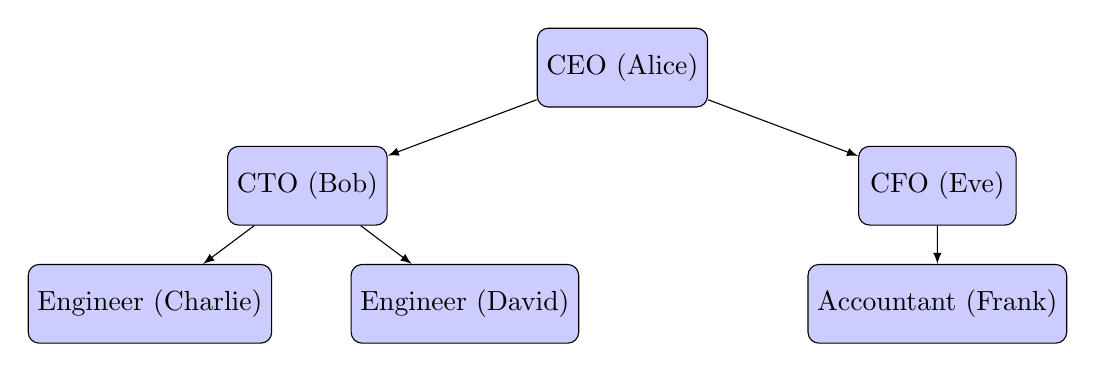
\begin{tikzpicture}[
		level 1/.style={sibling distance=80mm},
		level 2/.style={sibling distance=40mm},
		edge from parent/.style={draw,-latex},
		every node/.style={draw,rounded corners,fill=blue!20,minimum width=2cm,minimum height=1cm,align=center}
		]
		
		\node {CEO (Alice)}
		child {node {CTO (Bob)}
			child {node {Engineer (Charlie)}}
			child {node {Engineer (David)}}
		}
		child {node {CFO (Eve)}
			child {node {Accountant (Frank)}}
		};
		
	\end{tikzpicture}
\end{center}


\subsection{Contoh Input dan Output}

\begin{itemize}
	\item \textbf{Mencari Atasan dari Charlie:} Bob
	\item \textbf{Mencari Atasan Hingga CEO dari David:} [Bob, Alice]
	\item \textbf{Mencari Bawahan Langsung dari Bob:} [Charlie, David]
	\item \textbf{Mencari Semua Bawahan dari Bob:} [Charlie, David]
\end{itemize}

\subsection{Petunjuk:}

\begin{itemize}
	\item Representasikan struktur organisasi menggunakan struktur data tree, di mana setiap node memiliki atribut nama karyawan dan referensi ke bawahan (child nodes).
	\item Gunakan traversal pohon, baik depth-first search (DFS) atau breadth-first search (BFS), untuk menyelesaikan fungsi-fungsi pencarian atasan dan bawahan.
	\item Untuk fungsi yang mencari semua bawahan, Anda bisa menggunakan algoritma rekursif untuk mengunjungi seluruh subtree dari karyawan yang bersangkutan.
	\item Uji setiap fungsi dengan beberapa nama karyawan yang berbeda dalam struktur organisasi untuk memastikan bahwa fungsi-fungsi tersebut bekerja dengan baik.
\end{itemize}

Tugas Anda adalah mengimplementasikan fungsi-fungsi tersebut dalam bahasa pemrograman Java.

\subsection{Kode Awal:}
\begin{lstlisting}[style=JavaStyle]
	import java.util.ArrayList;
	import java.util.List;
	
	// Class representing a node in the tree
	class TreeNode {
		private String position;  // Job position (e.g., CEO, CTO, Engineer)
		private String name;      // Name of the person (e.g., Alice, Bob)
		private List<TreeNode> children;  // List of child nodes (subordinates)
		
		public TreeNode(String position, String name) {
			this.position = position;
			this.name = name;
			this.children = new ArrayList<>();
		}
		
		public void addChild(TreeNode child) {
			children.add(child);
		}
		
		public List<TreeNode> getChildren() {
			return children;
		}
		
		public String getPosition() {
			return position;
		}
		
		public String getName() {
			return name;
		}
		
		@Override
		public String toString() {
			return position + " (" + name + ")";
		}
		
		// Recursive function to print the tree structure
		public void printTree(String prefix) {
			System.out.println(prefix + toString());
			for (TreeNode child : children) {
				child.printTree(prefix + "    ");
			}
		}
	}
	
	// Main class to demonstrate the tree structure
	public class Main {
		public static void main(String[] args) {
			// Create the root node (CEO)
			TreeNode ceo = new TreeNode("CEO", "Alice");
			
			// Create CTO node and its children
			TreeNode cto = new TreeNode("CTO", "Bob");
			TreeNode engineer1 = new TreeNode("Engineer", "Charlie");
			TreeNode engineer2 = new TreeNode("Engineer", "David");
			cto.addChild(engineer1);
			cto.addChild(engineer2);
			
			// Create CFO node and its child
			TreeNode cfo = new TreeNode("CFO", "Eve");
			TreeNode accountant = new TreeNode("Accountant", "Frank");
			cfo.addChild(accountant);
			
			// Add CTO and CFO to CEO
			ceo.addChild(cto);
			ceo.addChild(cfo);
			
			// Print the tree structure
			ceo.printTree("");
		}
	}
\end{lstlisting}


\section{Soal \textit{Graph}}

Diberikan sebuah graph yang merepresentasikan beberapa kota besar di dunia beserta jarak antar kota-kota tersebut. Setiap node merepresentasikan sebuah kota, dan setiap edge (sisi) merepresentasikan jarak antara dua kota.


\begin{enumerate}
	\item \textbf{Cari Jarak dari Kota A ke Kota B} \\
	Buatlah fungsi yang menerima dua parameter, yaitu nama kota A dan kota B, dan mengembalikan jarak antara kedua kota tersebut berdasarkan graph yang sudah diberikan.
	
	\item \textbf{Tampilkan Kota-Kota yang Dilalui dari Kota A ke Kota B} \\
	Buat fungsi yang menampilkan daftar kota-kota yang dilalui dalam perjalanan dari kota A ke kota B berdasarkan rute yang ada di graph.
	
	\item \textbf{Cari Jalur Terpendek dari Kota A ke Kota B} \\
	Buat fungsi untuk mencari dan menampilkan jalur terpendek dari kota A ke kota B, serta menampilkan total jaraknya.
	
	\item \textbf{Cari Jalur Terpanjang dari Kota A ke Kota B} \\
	Buat fungsi untuk mencari dan menampilkan jalur terpanjang dari kota A ke kota B, serta menampilkan total jaraknya.
\end{enumerate}

Berikut adalah contoh graph yang merepresentasikan beberapa kota besar di dunia beserta jarak antar kota:

\begin{center}
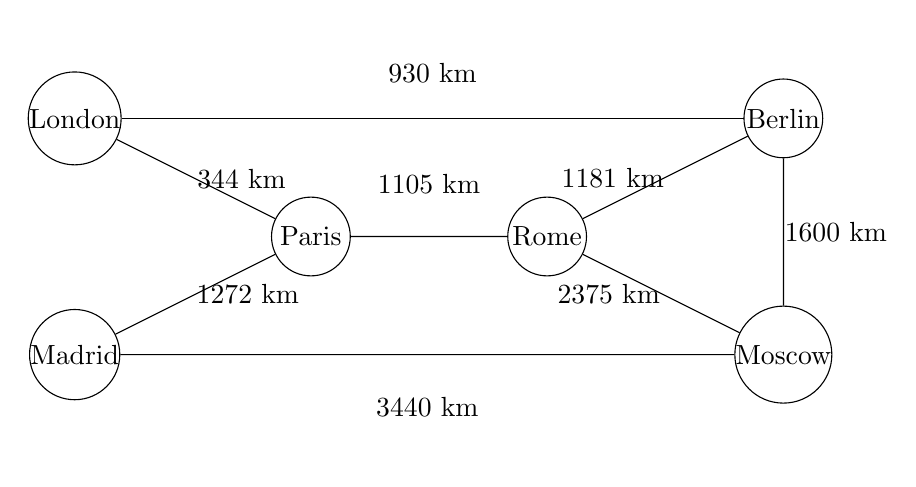
\begin{tikzpicture}[scale=1.5, every node/.style={circle, draw, minimum size=1cm, inner sep=0pt}]
	% Define the nodes (cities)
	\node (London) at (0, 0) {London};
	\node (Paris) at (2, -1) {Paris};
	\node (Berlin) at (6, 0) {Berlin};
	\node (Rome) at (4, -1) {Rome};
	\node (Madrid) at (0, -2) {Madrid};
	\node (Moscow) at (6, -2) {Moscow};
	
	% Draw edges with distances
	\draw (London) -- (Paris) node[midway, right, draw=none] {344 km};
	\draw (London) -- (Berlin) node[midway, above, draw=none] {930 km};
	\draw (Paris) -- (Rome) node[midway, above, draw=none] {1105 km};
	\draw (Berlin) -- (Rome) node[midway, left, draw=none] {1181 km};
	\draw (Paris) -- (Madrid) node[midway, right, draw=none] {1272 km};
	\draw (Berlin) -- (Moscow) node[midway, right, draw=none] {1600 km};
	\draw (Rome) -- (Moscow) node[midway, left, draw=none] {2375 km};
	\draw (Madrid) -- (Moscow) node[midway, below, draw=none] {3440 km};
\end{tikzpicture}
\end{center}
\[
\begin{array}{c|c|c}
	\textbf{Kota A} & \textbf{Kota B} & \textbf{Jarak (km)} \\
	\hline
	London & Paris & 344 \\
	London & Berlin & 930 \\
	Paris  & Rome  & 1105 \\
	Berlin & Rome  & 1181 \\
	Paris  & Madrid & 1272 \\
	Berlin & Moscow & 1600 \\
	Rome   & Moscow & 2375 \\
	Madrid & Moscow & 3440 \\
\end{array}
\]

\subsection{Petunjuk:}

\begin{itemize}
	\item Gunakan struktur data \textit{graph} untuk menyimpan kota-kota beserta jarak antar kota.
	\item Implementasikan tiga kelas berikut:
	\begin{itemize}
		\item \textbf{Graph}: Kelas ini merepresentasikan keseluruhan graph dan menyimpan node dan edge.
		\item \textbf{Node}: Kelas ini merepresentasikan kota, yang memiliki atribut seperti nama kota.
		\item \textbf{Edge}: Kelas ini menghubungkan dua kota (node) dan memiliki atribut untuk menyimpan jarak antara kedua kota tersebut.
	\end{itemize}
	\item Buat fungsi untuk mencari jalur terpendek dari 2 kota.
	\item Lakukan hal yang sama untuk mencari jalur terpanjang antara 2 kota.
	\item Tampilkan juga kota apa saja yang dilewati.
\end{itemize}

Tugas Anda adalah mengimplementasikan fungsi-fungsi tersebut dalam bahasa pemrograman Java.

\subsection{Kode Awal:}
\begin{lstlisting}[style=JavaStyle]
	class Node {
		private String cityName;
		
		public Node(String cityName) {
			this.cityName = cityName;
		}
		
		public String getCityName() {
			return cityName;
		}
		
		@Override
		public String toString() {
			return cityName;
		}
	}
	
	class Edge {
		private Node node1;
		private Node node2;
		private int distance; // Distance between the two nodes
		
		public Edge(Node node1, Node node2, int distance) {
			this.node1 = node1;
			this.node2 = node2;
			this.distance = distance;
		}
		
		public Node getNode1() {
			return node1;
		}
		
		public Node getNode2() {
			return node2;
		}
		
		public int getDistance() {
			return distance;
		}
		
		@Override
		public String toString() {
			return node1 + " <--> " + node2 + ": " + distance + " km";
		}
	}
	
	import java.util.ArrayList;
	import java.util.List;
	
	class Graph {
		private List<Node> nodes;
		private List<Edge> edges;
		
		public Graph() {
			nodes = new ArrayList<>();
			edges = new ArrayList<>();
		}
		
		public void addNode(Node node) {
			nodes.add(node);
		}
		
		public void addEdge(Node node1, Node node2, int distance) {
			Edge edge = new Edge(node1, node2, distance);
			edges.add(edge);
		}
		
		public void displayGraph() {
			for (Edge edge : edges) {
				System.out.println(edge);
			}
		}
	}
	
	public class Main {
		public static void main(String[] args) {
			// Create a new graph
			Graph graph = new Graph();
			
			// Create nodes (cities)
			Node london = new Node("London");
			Node paris = new Node("Paris");
			Node berlin = new Node("Berlin");
			Node rome = new Node("Rome");
			Node madrid = new Node("Madrid");
			Node moscow = new Node("Moscow");
			
			// Add nodes to the graph
			graph.addNode(london);
			graph.addNode(paris);
			graph.addNode(berlin);
			graph.addNode(rome);
			graph.addNode(madrid);
			graph.addNode(moscow);
			
			// Add edges with distances
			graph.addEdge(london, paris, 344);
			graph.addEdge(london, berlin, 930);
			graph.addEdge(paris, rome, 1105);
			graph.addEdge(berlin, rome, 1181);
			graph.addEdge(paris, madrid, 1272);
			graph.addEdge(berlin, moscow, 1600);
			graph.addEdge(rome, moscow, 2375);
			graph.addEdge(madrid, moscow, 3440);
			
			// Display the graph
			graph.displayGraph();
		}
	}
\end{lstlisting}




	\chapter{Abstrak dan Pewarisan (Inheritance)}

\section{Kelas Abstrak dan Pewarisan (Inheritance) di Java}

\subsection{Kelas Abstrak}

Kelas abstrak adalah kelas yang tidak dapat diinstansiasi dan sering digunakan sebagai dasar untuk kelas lain. Kelas ini dapat memiliki metode abstrak (metode tanpa implementasi) yang harus diimplementasikan oleh kelas turunannya. Kelas abstrak juga dapat memiliki metode konkret (metode dengan implementasi).

\textbf{Contoh Kelas Abstrak:}

\begin{lstlisting}[style=JavaStyle]
	package edu.example;
	
	public abstract class Shape {
		private String color;
		
		public Shape(String color) {
			this.color = color;
		}
		
		public String getColor() {
			return color;
		}
		
		public abstract double getArea();
	}
\end{lstlisting}

Pada contoh di atas, kelas \texttt{Shape} adalah kelas abstrak yang memiliki metode abstrak \texttt{getArea()} yang harus diimplementasikan oleh kelas turunannya. Kelas ini juga memiliki metode konkret \texttt{getColor()}.

\subsection{Pewarisan (Inheritance)}

Pewarisan memungkinkan sebuah kelas (kelas turunan) untuk mewarisi atribut dan metode dari kelas lain (kelas dasar). Ini memungkinkan penggunaan kembali kode dan mendukung hierarki kelas. Kelas turunan dapat mengakses metode dan atribut dari kelas dasar, serta menambahkan atau memodifikasi fungsionalitas sesuai kebutuhan.

\textbf{Contoh Pewarisan:}

\begin{lstlisting}[style=JavaStyle]
	package edu.example;
	
	public class Rectangle extends Shape {
		private double width;
		private double height;
		
		public Rectangle(String color, double width, double height) {
			super(color);
			this.width = width;
			this.height = height;
		}
		
		@Override
		public double getArea() {
			return width * height;
		}
		
		public double getWidth() {
			return width;
		}
		
		public double getHeight() {
			return height;
		}
	}
\end{lstlisting}

\subsection{Override}

\texttt{Override} adalah konsep dalam pewarisan di mana sebuah metode di kelas turunan menggantikan atau mengubah implementasi dari metode yang diwarisi dari kelas dasar. Kata kunci \texttt{@Override} digunakan untuk menunjukkan bahwa metode tersebut dimaksudkan untuk menggantikan metode yang ada di kelas dasar. Ini membantu menghindari kesalahan dan memastikan bahwa metode yang ditulis benar-benar menggantikan metode di kelas dasar.

\textbf{Contoh Override:}

\begin{lstlisting}[style=JavaStyle]
	@Override
	public double getArea() {
		return width * height;
	}
\end{lstlisting}

Pada contoh di atas, metode \texttt{getArea()} yang dideklarasikan dalam kelas \texttt{Rectangle} menggantikan metode \texttt{getArea()} yang dideklarasikan dalam kelas \texttt{Shape}. Dengan menggunakan \texttt{@Override}, kita menandakan bahwa metode ini menggantikan implementasi metode yang sama dari kelas dasar, sehingga meningkatkan kejelasan dan mencegah potensi kesalahan.

\subsection{Interface}

\textbf{Interface} adalah sebuah kontrak dalam pemrograman berorientasi objek yang mendefinisikan metode tanpa memberikan implementasinya. Interface berguna untuk mendefinisikan perilaku umum yang harus dimiliki oleh berbagai kelas tanpa memerlukan pewarisan langsung. Setiap kelas yang mengimplementasikan sebuah interface harus menyediakan implementasi untuk semua metode yang didefinisikan dalam interface tersebut.

\textbf{Contoh Interface:}

\begin{lstlisting}[style=JavaStyle, caption={Drawable.java}]
	package edu.example;
	
	public interface Drawable {
		void draw();
	}
\end{lstlisting}

Pada contoh di atas, \texttt{Drawable} adalah interface dengan metode \texttt{draw()} yang harus diimplementasikan oleh kelas apa pun yang mengimplementasikan interface ini. Interface ini memungkinkan berbagai kelas untuk memiliki metode \texttt{draw()} dengan cara yang sesuai dengan kelas masing-masing.

\subsection{Implementasi Kelas \texttt{Rectangle}}

Kelas \texttt{Rectangle} adalah salah satu kelas turunan dari \texttt{Shape} yang juga mengimplementasikan interface \texttt{Drawable}. Kelas ini memiliki atribut untuk lebar (\texttt{width}) dan tinggi (\texttt{height}) serta metode untuk menghitung luas dan menggambar persegi panjang.

\begin{lstlisting}[style=JavaStyle]
	package edu.example;
	
	public class Rectangle extends Shape implements Drawable {
		private double width;
		private double height;
		
		public Rectangle(String color, double width, double height) {
			super(color);
			this.width = width;
			this.height = height;
		}
		
		@Override
		public double getArea() {
			return width * height;
		}
		
		@Override
		public void draw() {
			System.out.println("Drawing a rectangle with width " + width + " and height " + height);
		}
	}
\end{lstlisting}

Pada contoh di atas, kelas \texttt{Rectangle} mengimplementasikan interface \texttt{Drawable} dan menyediakan implementasi untuk metode \texttt{draw()}. Selain itu, kelas ini mengoverride metode abstrak \texttt{getArea()} dari \texttt{Shape} untuk menghitung luas persegi panjang.

\subsection{Implementasi Kelas \texttt{Triangle}}

Sebagai tambahan dari \texttt{Rectangle}, kita juga dapat membuat kelas \texttt{Triangle} yang mengimplementasikan interface \texttt{Drawable} dan mewarisi kelas abstrak \texttt{Shape}. Kelas \texttt{Triangle} ini akan memiliki metode untuk menghitung luas dan menggambar segitiga.

\begin{lstlisting}[style=JavaStyle]
	package edu.example;
	
	public class Triangle extends Shape implements Drawable {
		private double base;
		private double height;
		
		public Triangle(String color, double base, double height) {
			super(color);
			this.base = base;
			this.height = height;
		}
		
		@Override
		public double getArea() {
			return 0.5 * base * height;
		}
		
		@Override
		public void draw() {
			System.out.println("Drawing a triangle with base " + base + " and height " + height);
		}
	}
\end{lstlisting}

Pada contoh di atas, kelas \texttt{Triangle} mengimplementasikan interface \texttt{Drawable} dan menyediakan implementasi untuk metode \texttt{draw()}. Selain itu, kelas ini mengoverride metode abstrak \texttt{getArea()} untuk menghitung luas segitiga.

\subsection{Demonstrasi Polimorfisme dengan \texttt{Rectangle} dan \texttt{Triangle}}

Polimorfisme memungkinkan kita untuk menggunakan objek \texttt{Rectangle} dan \texttt{Triangle} secara seragam melalui referensi kelas abstrak \texttt{Shape} atau interface \texttt{Drawable}. Berikut adalah contoh kode yang menunjukkan cara menggunakan polimorfisme dalam program untuk menggambar dan menghitung luas bentuk-bentuk ini.

\begin{lstlisting}[style=JavaStyle]
	package edu.example;
	
	public class ShapeDemo {
		public static void main(String[] args) {
			Shape[] shapes = {
				new Rectangle("blue", 4, 5),
				new Triangle("green", 3, 6)
			};
			
			for (Shape shape : shapes) {
				System.out.println("Color: " + shape.getColor());
				System.out.println("Area: " + shape.getArea());
				
				if (shape instanceof Drawable) {
					((Drawable) shape).draw();
				}
				
				System.out.println();
			}
		}
	}
\end{lstlisting}

\textbf{Penjelasan Kode:}
Pada contoh di atas, array \texttt{shapes} berisi objek \texttt{Rectangle} dan \texttt{Triangle}. Dengan menggunakan referensi \texttt{Shape}, kita dapat memanggil metode \texttt{getColor()} dan \texttt{getArea()} untuk masing-masing objek tanpa harus mengetahui tipe spesifiknya. Selain itu, kita menggunakan polimorfisme dengan interface \texttt{Drawable} untuk memanggil metode \texttt{draw()} pada objek yang mengimplementasikan interface ini.


\subsection{Implementasi dan Penggunaan}

Kelas abstrak, pewarisan, dan \texttt{override} digunakan untuk membangun struktur hierarki yang lebih kompleks dengan kode yang dapat digunakan kembali. Kelas turunan dapat memperluas fungsionalitas kelas dasar, menyesuaikan perilaku metode, dan memperbaiki implementasi metode abstrak sesuai dengan kebutuhan aplikasi.

\section{Contoh Implementasi Kode Abstrak dan Pewarisan di Java}

\subsection{Kelas \texttt{Question}}

\begin{lstlisting}[style=JavaStyle]
	package edu.pradita;
	
	public abstract class Question {
		
		private String text;
		private Object correctAnswer;
		
		public Question(String text, Object correctAnswer) {
			this.text = text;
			this.correctAnswer = correctAnswer;
		}
		
		public void display() {
			System.out.println(this.getText());
		}
		
		public boolean checkSubmittedAnswer(Object submittedAnswer) {
			if (correctAnswer.equals(submittedAnswer)) {
				return true;
			} else {
				return false;
			}
		}
		
		public String getText() {
			return text;
		}
		
		public Object getCorrectAnswer() {
			return correctAnswer;
		}
	}
\end{lstlisting}

\textbf{Penjelasan:} Kelas \texttt{Question} adalah kelas abstrak yang menyimpan informasi umum tentang pertanyaan, termasuk teks pertanyaan dan jawaban yang benar. Metode \texttt{display()} menampilkan teks pertanyaan, dan metode \texttt{checkSubmittedAnswer(Object submittedAnswer)} memeriksa apakah jawaban yang diberikan sesuai dengan jawaban yang benar.

\subsection{Kelas \texttt{OpenQuestion}}

\begin{lstlisting}[style=JavaStyle]
	package edu.pradita;
	
	public class OpenQuestion extends Question {
		
		public OpenQuestion(String text) {
			super(text, null);
		}
		
		@Override
		public boolean checkSubmittedAnswer(Object submittedAnswer) {
			return true;
		}
	}
\end{lstlisting}

\textbf{Penjelasan:} Kelas \texttt{OpenQuestion} adalah turunan dari kelas \texttt{Question} untuk pertanyaan terbuka. Konstruktor hanya memerlukan teks pertanyaan dan tidak memerlukan jawaban yang benar. Metode \texttt{checkSubmittedAnswer(Object submittedAnswer)} selalu mengembalikan \texttt{true} karena semua jawaban dianggap benar.

\subsection{Kelas \texttt{NumericQuestion}}

\begin{lstlisting}[style=JavaStyle]
	package edu.pradita;
	
	public class NumericQuestion extends Question {
		
		public NumericQuestion(String text, int correctAnswer) {
			super(text, correctAnswer);
		}
		
		public NumericQuestion(String text, double correctAnswer) {
			super(text, correctAnswer);
		}
		
		@Override
		public boolean checkSubmittedAnswer(Object submittedAnswer) {
			return (double) this.getCorrectAnswer() == Double.valueOf(submittedAnswer.toString());
		}
	}
\end{lstlisting}

\textbf{Penjelasan:} Kelas \texttt{NumericQuestion} menangani pertanyaan dengan jawaban numerik. Terdapat dua konstruktor untuk menerima jawaban yang benar bertipe \texttt{int} atau \texttt{double}. Metode \texttt{checkSubmittedAnswer(Object submittedAnswer)} memeriksa apakah jawaban yang diberikan sesuai dengan jawaban numerik yang benar.

\subsection{Kelas \texttt{FilledInQuestion}}

\begin{lstlisting}[style=JavaStyle]
	package edu.pradita;
	
	public class FilledInQuestion extends Question {
		
		public FilledInQuestion(String text, String correctAnswer) {
			super(text, correctAnswer);
		}
	}
\end{lstlisting}

\textbf{Penjelasan:} Kelas \texttt{FilledInQuestion} menangani pertanyaan dengan jawaban yang harus diisi. Konstruktor menerima teks pertanyaan dan jawaban yang benar bertipe \texttt{String}.

\subsection{Kelas \texttt{MultipleChoiceQuestion}}

\begin{lstlisting}[style=JavaStyle]
	package edu.pradita;
	
	import java.util.ArrayList;
	import java.util.List;
	
	public class MultipleChoiceQuestion extends Question {
		
		private List<Object> choices = new ArrayList<>();
		
		public MultipleChoiceQuestion(String text, Object correctAnswer, List<Object> choices) {
			super(text, correctAnswer);
			this.choices.addAll(choices);
		}
		
		@Override
		public void display() {
			display(true);
		}
		
		public void display(boolean withAbc) {
			super.display();
			int code = 97;
			for (Object choice : choices) {
				char head = '-';
				if (withAbc) {
					head = (char) code;
				}
				System.out.println(head + " " + choice);
				code++;
			}
		}
		
		public List<Object> getChoices() {
			return choices;
		}
	}
\end{lstlisting}

\textbf{Penjelasan:} Kelas \texttt{MultipleChoiceQuestion} menangani pertanyaan pilihan ganda. Selain teks pertanyaan dan jawaban yang benar, kelas ini juga menyimpan daftar pilihan jawaban. Metode \texttt{display()} menampilkan pertanyaan dan opsi jawaban dengan atau tanpa huruf ABC.

\subsection{Kelas \texttt{TrueFalseQuestion}}

\begin{lstlisting}[style=JavaStyle]
	package edu.pradita;
	
	import java.util.ArrayList;
	import java.util.Arrays;
	
	public class TrueFalseQuestion extends MultipleChoiceQuestion {
		
		public TrueFalseQuestion(String text, Object correctAnswer) {
			super(text, true, new ArrayList<>(Arrays.asList(true, false)));
		}
		
		@Override
		public boolean checkSubmittedAnswer(Object submittedAnswer) {
			return (boolean) this.getCorrectAnswer() == Boolean.valueOf(submittedAnswer.toString());
		}
	}
\end{lstlisting}

\textbf{Penjelasan:} Kelas \texttt{TrueFalseQuestion} adalah turunan dari \texttt{MultipleChoiceQuestion} khusus untuk pertanyaan benar/salah. Konstruktornya menerima teks pertanyaan dan jawaban yang benar, dan selalu menyertakan pilihan \texttt{true} dan \texttt{false}.

\subsection{Kelas \texttt{Main}}

\begin{lstlisting}[style=JavaStyle]
	package edu.pradita;
	
	import java.util.ArrayList;
	import java.util.Arrays;
	import java.util.List;
	import java.util.Scanner;
	
	public class Main {
		
		public static void main(String[] args) {
			
			List<Question> questions = new ArrayList<>();
			
			questions.add(new FilledInQuestion("He is __ farmer.", "a"));
			questions.add(new NumericQuestion("1 + 1 = ?", 2));
			questions.add(new OpenQuestion("What is your plan for the next semester?"));
			questions.add(new MultipleChoiceQuestion("_____ in the Wonderland.",
			"Alice",
			new ArrayList<>(Arrays.asList("Alice", "Bob", "Charlie"))
			));
			questions.add(new TrueFalseQuestion("Is today Tuesday?", true));
			
			Scanner scanner = new Scanner(System.in);
			
			for (int lineNum = 1; lineNum <= questions.size(); lineNum++) {
				Question question = questions.get(lineNum - 1);
				System.out.println("Question " + lineNum + ":");
				question.display();
				System.out.print("Your answer: ");
				String answer = scanner.nextLine().trim();
				boolean result = question.checkSubmittedAnswer(answer);
				System.out.println("Result: " + result);
				System.out.println();
			}
			
			scanner.close();
		}
	}
\end{lstlisting}

\textbf{Penjelasan:} Kelas \texttt{Main} adalah kelas utama yang menampilkan dan memproses daftar pertanyaan. Program membuat beberapa pertanyaan dari berbagai jenis, menambahkannya ke dalam daftar, dan kemudian menampilkan setiap pertanyaan satu per satu. Pengguna diminta untuk memberikan jawaban, yang kemudian diperiksa dengan metode \texttt{checkSubmittedAnswer()}. Hasil dari setiap jawaban ditampilkan setelah input.

\section{Latihan}


Kerjakanlah contoh-contoh kasus berikut! Ketik kode program dan jalankan! Amati struktur, output, dan perilaku program. Cobalah menjawab pertanyaan-pertanyaan yang diberikan untuk meningkatkan pemahaman mengenai konsep yang diajarkan dengan mengisi persegi kosong yang sediakan.

\subsection{Contoh Sistem Pembayaran Online}

\subsubsection{Langkah 1: Kelas Abstrak dan Pewarisan}

\textbf{Kode:} Mendefinisikan kelas abstrak \texttt{Payment} dan kelas konkret \texttt{CreditCardPayment} dan \texttt{PayPalPayment}.

\begin{lstlisting}[style=JavaStyle, caption={Payment.java}]
	package com.example.payment;
	
	public abstract class Payment {
		double amount;
		
		public Payment(double amount) {
			this.amount = amount;
		}
		
		public abstract void processPayment();
		
		public void displayAmount() {
			System.out.println("Payment Amount: $" + amount);
		}
	}
\end{lstlisting}

\begin{lstlisting}[style=JavaStyle, caption={CreditCardPayment.java}]
	package com.example.payment.types;
	
	import com.example.payment.Payment;
	
	public class CreditCardPayment extends Payment {
		public CreditCardPayment(double amount) {
			super(amount);
		}
		
		@Override
		public void processPayment() {
			System.out.println("Processing credit card payment of $" + amount);
		}
	}
\end{lstlisting}

\begin{lstlisting}[style=JavaStyle, caption={PayPalPayment.java}]
	package com.example.payment.types;
	
	import com.example.payment.Payment;
	
	public class PayPalPayment extends Payment {
		public PayPalPayment(double amount) {
			super(amount);
		}
		
		@Override
		public void displayAmount() {
			System.out.println("Payment Amount: USD" + amount);
		}
		
		@Override
		public void processPayment() {
			System.out.println("Processing PayPal payment of USD" + amount);
		}
	}
\end{lstlisting}

\textbf{Pertanyaan Refleksi:}
\begin{enumerate}
	\item Cobalah buat object dari kelas abstrak dalam metode \texttt{main}! Coba jalankan program. Bagaimankah hasilnya? Mengapa demikian?
	\begin{lstlisting}[style=JavaStyle, caption={TestAbstractClassInstantiation.java}]
		package com.example.payment.system;
		
		import com.example.payment.Payment;
		
		public class TestAbstractClassInstantiation {
			public static void main(String[] args) {
				Payment payment = new Payment(100.0);
				System.out.println("End");
			}
		}
	\end{lstlisting}
	\begin{tcolorbox}[colback=white, colframe=black,  width=\linewidth, height=3cm,  boxrule=1pt, sharp corners]
	\end{tcolorbox}
	\item Coba buat objek dari kelas-kelas yang di-\texttt{extends} dari kelas abstrak? Coba jalankan program. Bagaimankah hasilnya? Mengapa demikian?
	\begin{lstlisting}[style=JavaStyle, caption={TestSubclassInstantiation.java}]
		package com.example.payment.system;
		
		import com.example.payment.Payment;
		import com.example.payment.types.CreditCardPayment;
		import com.example.payment.types.PayPalPayment;
		
		public class TestSubclassInstantiation {
			public static void main(String[] args) {
				// Membuat objek dari kelas-kelas turunan
				Payment creditCardPayment = new CreditCardPayment(200.0);
				Payment payPalPayment = new PayPalPayment(150.0);
				System.out.println("End");
			}
		}
	\end{lstlisting}
	\begin{tcolorbox}[colback=white, colframe=black,  width=\linewidth, height=3cm,  boxrule=1pt, sharp corners]
	\end{tcolorbox}
	\item Coba hapus metode \texttt{processPayment()} dari kelas-kelas yang di-extends dari kelas abstrak. Coba jalankan program. Bagaimankah hasilnya? Mengapa demikian?
	\begin{lstlisting}[style=JavaStyle, caption={TestSubclassInstantiation.java}]
		package com.example.payment.system;
		
		import com.example.payment.Payment;
		import com.example.payment.types.CreditCardPayment;
		import com.example.payment.types.PayPalPayment;
		
		public class TestSubclassInstantiation {
			public static void main(String[] args) {
				// Membuat objek dari kelas-kelas turunan
				Payment creditCardPayment = new CreditCardPayment(200.0);
				Payment payPalPayment = new PayPalPayment(150.0);
				
				// Memproses setiap pembayaran
				creditCardPayment.processPayment();
				creditCardPayment.displayAmount();
				
				System.out.println();
				
				payPalPayment.processPayment();
				payPalPayment.displayAmount();
				
				System.out.println("End");
			}
		}
	\end{lstlisting}
	\begin{tcolorbox}[colback=white, colframe=black,  width=\linewidth, height=3cm,  boxrule=1pt, sharp corners]
	\end{tcolorbox}
	\item Mengapa \texttt{creditCardPayment} dapat menampilkan \texttt{Payment Amount: \$} walaupun metode untuk menampilkan teks tersebut TIDAK terdapat dalam kelas \texttt{creditCardPayment}?
	\begin{tcolorbox}[colback=white, colframe=black,  width=\linewidth, height=3cm,  boxrule=1pt, sharp corners]
	\end{tcolorbox}
	\item Mengapa objek \texttt{paypalPayment} menampilkan \texttt{Payment Amount: \textbf{USD}} sedangkan \texttt{creditCardPayment} menampikan \texttt{Payment Amount: \textbf{\$}}?
	\begin{tcolorbox}[colback=white, colframe=black,  width=\linewidth, height=3cm,  boxrule=1pt, sharp corners]
	\end{tcolorbox}
	\item Mengapa \texttt{Payment} didefinisikan sebagai kelas abstrak daripada kelas biasa?
	\begin{tcolorbox}[colback=white, colframe=black,  width=\linewidth, height=3cm,  boxrule=1pt, sharp corners]
	\end{tcolorbox}
	\item Bagaimana pewarisan dari \texttt{Payment} ke \texttt{CreditCardPayment} dan \texttt{PayPalPayment} mengurangi redundansi?
	\begin{tcolorbox}[colback=white, colframe=black,  width=\linewidth, height=3cm,  boxrule=1pt, sharp corners]
	\end{tcolorbox}
	\item Apa manfaat dari struktur ini jika kita ingin menambahkan metode pembayaran baru di masa depan?
	\begin{tcolorbox}[colback=white, colframe=black,  width=\linewidth, height=3cm,  boxrule=1pt, sharp corners]
	\end{tcolorbox}
\end{enumerate}

\subsubsection{Langkah 2: Implementasi Interface}

\textbf{Kode:} Mengimplementasikan antarmuka \texttt{Refundable} untuk \texttt{DebitCardPayment}.

\begin{lstlisting}[style=JavaStyle, caption={Refundable.java}]
	package com.example.payment.features;
	
	public interface Refundable {
		void refund();
	}
\end{lstlisting}

\begin{lstlisting}[style=JavaStyle, caption={DebitCardPayment.java}]
	package com.example.payment.types;
	
	import com.example.payment.Payment;
	import com.example.payment.features.Refundable;
	
	public class DebitCardPayment extends Payment implements Refundable {
		public DebitCardPayment(double amount) {
			super(amount);
		}
		
		@Override
		public void processPayment() {
			System.out.println("Processing debit card payment of $" + amount);
		}
		
		@Override
		public void refund() {
			System.out.println("Refunding debit card payment of $" + amount);
		}
	}
\end{lstlisting}

\begin{lstlisting}[style=JavaStyle, caption={PaymentApp.java}]
	package com.example.payment;
	
	import com.example.payment.types.DebitCardPayment;
	
	public class PaymentApp {
		public static void main(String[] args) {
			// Membuat objek dari kelas DebitCardPayment
			DebitCardPayment debitCardPayment = new DebitCardPayment(100.0);
			
			// Memproses pembayaran
			debitCardPayment.processPayment();
			
			// Melakukan pengembalian dana (refund)
			debitCardPayment.refund();
		}
	}
\end{lstlisting}

\textbf{Pertanyaan Refleksi:}
\begin{enumerate}
	\item Coba hapus metode \texttt{refund()} yang ada di dalam kelas yang mengimplementasikan (\texttt{implements}) \texttt{Refundable}, bukan yang ada di dalam \texttt{interface}? Coba jalankan program. Apa yang terjadi? Mengapa demikian?
	\begin{tcolorbox}[colback=white, colframe=black,  width=\linewidth, height=3cm,  boxrule=1pt, sharp corners]
	\end{tcolorbox}
	\item Bagaimana penerapan antarmuka \texttt{Refundable} memengaruhi kelas \texttt{DebitCardPayment}?
	\begin{tcolorbox}[colback=white, colframe=black,  width=\linewidth, height=3cm,  boxrule=1pt, sharp corners]
	\end{tcolorbox}
	\item Apa keuntungan dari menggunakan antarmuka seperti \texttt{Refundable} dalam sistem pembayaran?
	\begin{tcolorbox}[colback=white, colframe=black,  width=\linewidth, height=3cm,  boxrule=1pt, sharp corners]
	\end{tcolorbox}
	\item Bagaimana desain ini memudahkan penambahan tipe pembayaran baru yang mendukung pengembalian dana di masa depan?
	\begin{tcolorbox}[colback=white, colframe=black,  width=\linewidth, height=3cm,  boxrule=1pt, sharp corners]
	\end{tcolorbox}
\end{enumerate}

\subsubsection{Langkah 3: Demonstrasi Polimorfisme}

Ubah 2 kelas \texttt{*Payment} sebelumnya dengan mengimplementasikan interface \texttt{Refundable} pada kedua kelas tersebut! 

\begin{lstlisting}[style=JavaStyle, caption={CreditCardPayment.java}]
	package com.example.payment.types;
	
	import com.example.payment.Payment;
	import com.example.payment.features.Refundable;
	
	public class CreditCardPayment extends Payment implements Refundable {
		public CreditCardPayment(double amount) {
			super(amount);
		}
		
		@Override
		public void processPayment() {
			System.out.println("Processing credit card payment of $" + amount);
		}
		
		@Override
		public void refund() {
			System.out.println("Refunding credit card payment of $" + amount);
		}
	}
\end{lstlisting}

\begin{lstlisting}[style=JavaStyle, caption={PayPalPayment.java}]
	package com.example.payment.types;
	
	import com.example.payment.Payment;
	import com.example.payment.features.Refundable;
	
	public class PayPalPayment extends Payment implements Refundable {
		public PayPalPayment(double amount) {
			super(amount);
		}
		
		@Override
		public void displayAmount() {
			System.out.println("Payment Amount: USD" + amount);
		}
		
		@Override
		public void processPayment() {
			System.out.println("Processing PayPal payment of USD" + amount);
		}
		
		@Override
		public void refund() {
			System.out.println("Refunding PayPal payment of USD" + amount);
		}
	}
\end{lstlisting}

Buat dan jalankan kode berikut kelas \texttt{PaymentSystem}. 

\begin{lstlisting}[style=JavaStyle, caption={PaymentSystem.java}]
	package com.example.payment.system;
	
	import com.example.payment.Payment;
	import com.example.payment.features.Refundable;
	import com.example.payment.types.CreditCardPayment;
	import com.example.payment.types.PayPalPayment;
	import com.example.payment.types.DebitCardPayment;
	
	public class PaymentSystem {
		public static void main(String[] args) {
			Payment[] payments = {
				new CreditCardPayment(100),
				new PayPalPayment(150),
				new DebitCardPayment(200)
			};
			
			for (Payment payment : payments) {
				payment.processPayment();
				if (payment instanceof Refundable) {
					((Refundable) payment).refund();
				}
			}
		}
	}
\end{lstlisting}

\textbf{Pertanyaan Refleksi:}
\begin{enumerate}
	\item Mengapa masing-masing objek menampilkan output yang berbeda walaupun mereka sama-sama mengeksekusi metode \texttt{refund}?
	\begin{tcolorbox}[colback=white, colframe=black,  width=\linewidth, height=3cm,  boxrule=1pt, sharp corners]
	\end{tcolorbox}
	\item Bagaimana polimorfisme memungkinkan kita untuk menangani berbagai jenis pembayaran menggunakan referensi \texttt{Payment} tunggal?
	\begin{tcolorbox}[colback=white, colframe=black,  width=\linewidth, height=3cm,  boxrule=1pt, sharp corners]
	\end{tcolorbox}
	\item Mengapa polimorfisme bermanfaat untuk menangani berbagai metode pembayaran dengan cara yang lebih fleksibel?
	\begin{tcolorbox}[colback=white, colframe=black,  width=\linewidth, height=3cm,  boxrule=1pt, sharp corners]
	\end{tcolorbox}
	\item Jelaskan bagaimana desain ini akan mendukung penambahan tipe pembayaran tambahan dengan perubahan kode minimal.
	\begin{tcolorbox}[colback=white, colframe=black,  width=\linewidth, height=3cm,  boxrule=1pt, sharp corners]
	\end{tcolorbox}
\end{enumerate}



\subsubsection{Langkah 4: Menyimpulkan}
Dari eksperimen di atas, buatlah pengertian dan manfaat dari konsep-konsep berikut dalam konteks pemrograman berorientasi objek dengan menggunakan kata-kata Anda sendiri.
\begin{enumerate}
	\item Kelas Abstrak
	\begin{tcolorbox}[colback=white, colframe=black,  width=\linewidth, height=3cm,  boxrule=1pt, sharp corners]
	\end{tcolorbox}
	\item Pewarisan/\textit{Inheritance} (\texttt{extends})
	\begin{tcolorbox}[colback=white, colframe=black,  width=\linewidth, height=3cm,  boxrule=1pt, sharp corners]
	\end{tcolorbox}
	\item Overriding
	\begin{tcolorbox}[colback=white, colframe=black,  width=\linewidth, height=3cm,  boxrule=1pt, sharp corners]
	\end{tcolorbox}
	\item Interface
	\begin{tcolorbox}[colback=white, colframe=black,  width=\linewidth, height=3cm,  boxrule=1pt, sharp corners]
	\end{tcolorbox}
	\item Polimorfisme
	\begin{tcolorbox}[colback=white, colframe=black,  width=\linewidth, height=3cm,  boxrule=1pt, sharp corners]
	\end{tcolorbox}
\end{enumerate}


\section{Soal}

Kerjakanlah contoh-contoh kasus berikut! Ketik kode program dan jalankan! Amati struktur, output, dan perilaku program. Cobalah menjawab pertanyaan-pertanyaan yang diberikan untuk meningkatkan pemahaman mengenai konsep yang diajarkan dengan mengisi persegi kosong yang sediakan.

\subsection{Contoh Sistem Pemesanan Transportasi}

\subsubsection{Langkah 1: Kelas Abstrak dan Pewarisan}

\textbf{Kode:} Mendefinisikan kelas abstrak \texttt{Vehicle} dan kelas konkret \texttt{Car} serta \texttt{Bus}.

\begin{lstlisting}[style=JavaStyle, caption={Vehicle.java}]
	package com.example.transport;
	
	public abstract class Vehicle {
		String id;
		
		public Vehicle(String id) {
			this.id = id;
		}
		
		public abstract double calculateFare(double distance);
		
		public void displayType() {
			System.out.println("Vehicle ID: " + id);
		}
	}
\end{lstlisting}

\begin{lstlisting}[style=JavaStyle, caption={Car.java}]
	package com.example.transport.types;
	
	import com.example.transport.Vehicle;
	
	public class Car extends Vehicle {
		public Car(String id) {
			super(id);
		}
		
		@Override
		public double calculateFare(double distance) {
			return distance * 0.5;
		}
	}
\end{lstlisting}

\begin{lstlisting}[style=JavaStyle, caption={Bus.java}]
	package com.example.transport.types;
	
	import com.example.transport.Vehicle;
	
	public class Bus extends Vehicle {
		public Bus(String id) {
			super(id);
		}
		
		@Override
		public double calculateFare(double distance) {
			return distance * 0.2;
		}
	}
\end{lstlisting}

\textbf{Pertanyaan Refleksi:}
\begin{enumerate}
	\item Cobalah buat objek dari kelas abstrak dalam metode \texttt{main}! Apa hasilnya? Mengapa demikian?
	\begin{tcolorbox}[colback=white, colframe=black,  width=\linewidth, height=3cm, boxrule=1pt, sharp corners]
	\end{tcolorbox}
	\item Coba buat objek dari kelas-kelas turunan dari kelas abstrak \texttt{Vehicle}. Apa hasilnya? Mengapa demikian?
	\begin{tcolorbox}[colback=white, colframe=black,  width=\linewidth, height=3cm, boxrule=1pt, sharp corners]
	\end{tcolorbox}
	\item Bagaimana mendefinisikan \texttt{Vehicle} sebagai kelas abstrak membantu mengelompokkan atribut dan metode umum untuk semua tipe kendaraan?
	\begin{tcolorbox}[colback=white, colframe=black, width=\linewidth, height=3cm, boxrule=1pt, sharp corners]
	\end{tcolorbox}
	\item Apa manfaat pewarisan saat mengimplementasikan tipe kendaraan yang berbeda seperti \texttt{Car} dan \texttt{Bus}?
	\begin{tcolorbox}[colback=white, colframe=black, width=\linewidth, height=3cm, boxrule=1pt, sharp corners]
	\end{tcolorbox}
	\item Dalam skenario apa Anda mempertimbangkan untuk menggunakan pola ini dalam aplikasi lain?
	\begin{tcolorbox}[colback=white, colframe=black, width=\linewidth, height=3cm, boxrule=1pt, sharp corners]
	\end{tcolorbox}
\end{enumerate}

\subsubsection{Langkah 2: Implementasi Interface}

\textbf{Kode:} Mengimplementasikan antarmuka \texttt{Trackable} untuk \texttt{Train}.

\begin{lstlisting}[style=JavaStyle, caption={Trackable.java}]
	package com.example.transport.features;
	
	public interface Trackable {
		void getLocation();
	}
\end{lstlisting}

\begin{lstlisting}[style=JavaStyle, caption={Train.java}]
	package com.example.transport.types;
	
	import com.example.transport.Vehicle;
	import com.example.transport.features.Trackable;
	
	public class Train extends Vehicle implements Trackable {
		public Train(String id) {
			super(id);
		}
		
		@Override
		public double calculateFare(double distance) {
			return distance * 0.3;
		}
		
		@Override
		public void getLocation() {
			System.out.println("Tracking train location for ID: " + id);
		}
	}
\end{lstlisting}

\textbf{Pertanyaan Refleksi:}
\begin{enumerate}
	\item Bagaimana antarmuka \texttt{Trackable} memungkinkan \texttt{Train} memiliki perilaku unik tanpa mengubah kelas \texttt{Vehicle}?
	\begin{tcolorbox}[colback=white, colframe=black,  width=\linewidth, height=3cm, boxrule=1pt, sharp corners]
	\end{tcolorbox}
	\item Mengapa memisahkan perilaku pelacakan lokasi ke dalam antarmuka merupakan hal yang bermanfaat?
	\begin{tcolorbox}[colback=white, colframe=black,  width=\linewidth, height=3cm, boxrule=1pt, sharp corners]
	\end{tcolorbox}
	\item Bagaimana Anda akan menggunakan antarmuka \texttt{Trackable} untuk tipe kendaraan lain yang memerlukan pelacakan?
	\begin{tcolorbox}[colback=white, colframe=black,  width=\linewidth, height=3cm, boxrule=1pt, sharp corners]
	\end{tcolorbox}
\end{enumerate}

\subsubsection{Langkah 3: Demonstrasi Polimorfisme}

\textbf{Kode:} Menunjukkan perilaku polimorfisme dengan kelas \texttt{BookingSystem}.

\begin{lstlisting}[style=JavaStyle, caption={BookingSystem.java}]
	package com.example.transport.system;
	
	import com.example.transport.Vehicle;
	import com.example.transport.features.Trackable;
	import com.example.transport.types.Car;
	import com.example.transport.types.Bus;
	import com.example.transport.types.Train;
	
	public class BookingSystem {
		public static void main(String[] args) {
			Vehicle[] vehicles = {
				new Car("C123"),
				new Bus("B456"),
				new Train("T789")
			};
			
			for (Vehicle vehicle : vehicles) {
				vehicle.displayType();
				System.out.println("Fare for 100 miles: $" + vehicle.calculateFare(100));
				if (vehicle instanceof Trackable) {
					((Trackable) vehicle).getLocation();
				}
			}
		}
	}
\end{lstlisting}

\textbf{Pertanyaan Refleksi:}
\begin{enumerate}
	\item Bagaimana polimorfisme memungkinkan kita menggunakan referensi \texttt{Vehicle} untuk mengelola berbagai jenis kendaraan?
	\begin{tcolorbox}[colback=white, colframe=black,  width=\linewidth, height=3cm, boxrule=1pt, sharp corners]
	\end{tcolorbox}
	\item Fleksibilitas apa yang ditambahkan oleh desain ini jika kita perlu menambahkan tipe kendaraan baru, seperti \texttt{Taxi}?
	\begin{tcolorbox}[colback=white, colframe=black,  width=\linewidth, height=3cm, boxrule=1pt, sharp corners]
	\end{tcolorbox}
	\item Mengapa polimorfisme berguna dalam sistem seperti sistem pemesanan transportasi?
	\begin{tcolorbox}[colback=white, colframe=black,  width=\linewidth, height=3cm, boxrule=1pt, sharp corners]
	\end{tcolorbox}
\end{enumerate}

%
%\subsection{Contoh Sistem Manajemen Karyawan}
%
%\subsubsection{Langkah 1: Kelas Abstrak dan Pewarisan}
%
%\textbf{Kode:} Mendefinisikan kelas abstrak \texttt{Employee} dan membuat subclass untuk \texttt{FullTimeEmployee} dan \texttt{PartTimeEmployee}.
%
%\begin{lstlisting}[style=JavaStyle, caption={Employee.java}]
%	package com.example.employee;
%	
%	public abstract class Employee {
	%		String name;
	%		
	%		public Employee(String name) {
		%			this.name = name;
		%		}
	%		
	%		public abstract double calculateCompensation();
	%		
	%		public void displayEmployee() {
		%			System.out.println("Employee Name: " + name);
		%		}
	%	}
%\end{lstlisting}
%
%\begin{lstlisting}[style=JavaStyle, caption={FullTimeEmployee.java dan PartTimeEmployee.java}]
%	package com.example.employee.types;
%	
%	import com.example.employee.Employee;
%	
%	public class FullTimeEmployee extends Employee {
	%		public FullTimeEmployee(String name) {
		%			super(name);
		%		}
	%		
	%		@Override
	%		public double calculateCompensation() {
		%			return 5000; // Gaji tetap
		%		}
	%	}
%	
%	public class PartTimeEmployee extends Employee {
	%		public PartTimeEmployee(String name) {
		%			super(name);
		%		}
	%		
	%		@Override
	%		public double calculateCompensation() {
		%			return 3000; // Gaji tetap
		%		}
	%	}
%\end{lstlisting}
%
%\textbf{Pertanyaan Refleksi:}
%\begin{itemize}
%	\item Cobalah buat object dari kelas abstrak dalam metode \texttt{main}! Apakah bisa atau tidak? Jika tidak bisa, mengapa?
%	\item Cobat buat objek dari kelas-kelas yang diturun dari kelas abstrak? Apakah bisa atau tidak? Jika bisa, mengapa?
%	\item Bagaimana menggunakan kelas abstrak \texttt{Employee} membantu standarisasi perilaku karyawan?
%	\item Apa manfaat pewarisan saat mendefinisikan tipe karyawan berbeda dengan metode kompensasi unik?
%	\item Dalam konteks apa lagi desain ini bisa diterapkan?
%\end{itemize}
%
%\subsubsection{Langkah 2: Implementasi Interface}
%
%\textbf{Kode:} Mengimplementasikan antarmuka \texttt{Promotable} untuk kelas \texttt{Contractor}.
%
%\begin{lstlisting}[style=JavaStyle, caption={Promotable.java}]
%	package com.example.employee.features;
%	
%	public interface Promotable {
	%		void promote();
	%	}
%\end{lstlisting}
%
%\begin{lstlisting}[style=JavaStyle, caption={Contractor.java}]
%	package com.example.employee.types;
%	
%	import com.example.employee.Employee;
%	import com.example.employee.features.Promotable;
%	
%	public class Contractor extends Employee implements Promotable {
	%		public Contractor(String name) {
		%			super(name);
		%		}
	%		
	%		@Override
	%		public double calculateCompensation() {
		%			return 4000; // Gaji tetap
		%		}
	%		
	%		@Override
	%		public void promote() {
		%			System.out.println("Promoting contractor: " + name);
		%		}
	%	}
%\end{lstlisting}
%
%\textbf{Pertanyaan Refleksi:}
%\begin{itemize}
%	\item Apa keuntungan dari antarmuka \texttt{Promotable} bagi kelas \texttt{Contractor}?
%	\item Mengapa kita memilih menggunakan antarmuka daripada menambahkan metode \texttt{promote} langsung ke \texttt{Employee}?
%	\item Bagaimana pendekatan ini memudahkan penerapan promosi untuk tipe karyawan tertentu?
%\end{itemize}
%
%\subsubsection{Langkah 3: Demonstrasi Polimorfisme}
%
%\textbf{Kode:} Menunjukkan perilaku polimorfisme dengan kelas \texttt{EmployeeManagementSystem}.
%
%\begin{lstlisting}[style=JavaStyle, caption={EmployeeManagementSystem.java}]
%	package com.example.employee.system;
%	
%	import com.example.employee.Employee;
%	import com.example.employee.features.Promotable;
%	import com.example.employee.types.FullTimeEmployee;
%	import com.example.employee.types.PartTimeEmployee;
%	import com.example.employee.types.Contractor;
%	
%	public class EmployeeManagementSystem {
	%		public static void main(String[] args) {
		%			Employee[] employees = {
			%				new FullTimeEmployee("Alice"),
			%				new PartTimeEmployee("Bob"),
			%				new Contractor("Charlie")
			%			};
		%			
		%			for (Employee employee : employees) {
			%				employee.displayEmployee();
			%				System.out.println("Compensation: $" + employee.calculateCompensation());
			%				if (employee instanceof Promotable) {
				%					((Promotable) employee).promote();
				%				}
			%			}
		%		}
	%	}
%\end{lstlisting}
%
%\textbf{Pertanyaan Refleksi:}
%\begin{itemize}
%	\item Bagaimana polimorfisme memungkinkan kita untuk menangani berbagai tipe karyawan melalui referensi \texttt{Employee} tunggal?
%	\item Bagaimana pendekatan ini mendukung skalabilitas jika tipe karyawan baru diperkenalkan?
%	\item Apa keuntungan polimorfisme dalam sistem yang mengelola berbagai jenis entitas seperti karyawan?
%\end{itemize}

	\chapter{Graphical User Interface}


\section{Pengenalan GUI di Java}

\subsection{Pengantar GUI di Java}
Graphical User Interface (GUI) di Java digunakan untuk membuat antarmuka pengguna yang interaktif dengan elemen-elemen visual seperti tombol, teks, label, dan lain-lain. Java menyediakan beberapa toolkit untuk membuat GUI, salah satunya adalah Swing, yang sangat populer digunakan.

Swing adalah bagian dari Java Foundation Classes (JFC) yang menyediakan alat dan komponen untuk membuat aplikasi desktop yang interaktif. Kelas utama dalam Swing meliputi \texttt{JFrame}, \texttt{JPanel}, \texttt{JLabel}, \texttt{JButton}, dan banyak lagi.

\subsection{Instalasi WindowBuilder di Eclipse}

\begin{enumerate}
	\item Buka Eclipse IDE.
	\item Pilih menu \texttt{Help} > \texttt{Install New Software}.
	\item Pada kotak \texttt{Work with}, pilih URL sesuai dengan versi eclipse yang kalian miliki
	\item Tekan \texttt{Enter}, dan Eclipse akan memuat daftar software yang tersedia dari URL tersebut.
	\item Centang opsi \texttt{WindowBuilder Swing Designer}, lalu klik \texttt{Next}.
	\item Ikuti petunjuk instalasi yang diberikan hingga selesai.
	\item Setelah instalasi selesai, restart Eclipse.
	\item WindowBuilder kini siap digunakan untuk membuat aplikasi GUI di Java.
\end{enumerate}


\subsection{Membuat GUI dengan WindowBuilder}

Setelah WindowBuilder diinstal, Anda bisa mulai membuat aplikasi GUI di Java dengan lebih mudah. WindowBuilder menyediakan editor drag-and-drop untuk menambahkan komponen GUI seperti tombol, label, dan panel tanpa perlu menulis kode secara manual.

Langkah-langkah membuat GUI menggunakan WindowBuilder:
\begin{enumerate}
	\item Buat project Java baru di Eclipse.
	\item Klik kanan pada package, pilih \texttt{New} > \texttt{Other}.
	\item Pilih \texttt{WindowBuilder} > \texttt{Swing Designer} > \texttt{JFrame}, lalu klik \texttt{Next}.
	\item Beri nama kelas dan klik \texttt{Finish}.
	\item Anda akan melihat editor GUI, di mana Anda dapat mendesain antarmuka dengan drag-and-drop komponen dari palet ke form.
	\item Tambahkan komponen yang diperlukan, seperti \texttt{JButton}, \texttt{JLabel}, \texttt{JTextField}, dll.
	\item Setelah selesai, simpan dan jalankan program untuk melihat GUI yang telah dibuat.
\end{enumerate}



\subsection{Opsional: Error pada WindowBuilder}

Jika terjadi error saat penggunaan WindowBuilder, ikuti langkah berikut:

\begin{enumerate}
	\item Buka Eclipse IDE.
	\item Pilih menu \texttt{Eclipse} > \texttt{Settings}.
	\item Pilih bagian \texttt{ Install/Update}, lalu pilih  \texttt{Available Software Sites}
	\item Uncheck bagian \texttt{Latest Eclipse IDE Packages Release} dan  \texttt{Latest Eclipse Simultaneaous Release}
	\item Klik \texttt{Apply and Close}
\end{enumerate}

\section{Contoh Kode dan Penjelasan}


\subsection{Frame Sederhana}

\textbf{Kode:} \texttt{SimpleFrame.java}

\textbf{Deskripsi:} Kode ini membuat jendela GUI sederhana dengan \texttt{JTextField}, \texttt{JButton}, dan \texttt{JLabel}. Ketika tombol diklik, label akan diperbarui untuk menampilkan pesan yang menyapa pengguna dengan nama yang dimasukkan.

\textbf{Penjelasan Kode:}
\begin{itemize}
	\item \texttt{SimpleFrame} adalah kelas yang memperluas \texttt{JFrame} untuk membuat jendela GUI.
	\item \texttt{JTextField} digunakan untuk memasukkan nama.
	\item \texttt{JButton} ketika diklik, akan memperbarui \texttt{JLabel} dengan pesan yang menyapa pengguna.
	\item Kode ini juga mengatur ukuran frame dengan \texttt{setSize}.
\end{itemize}

\textbf{Gambar:} \\
\begin{center}
	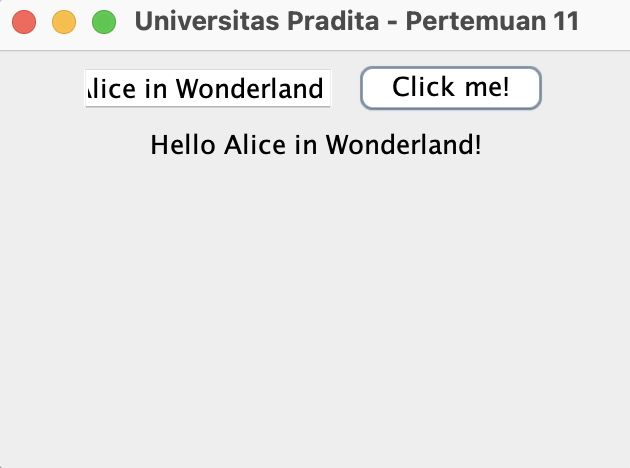
\includegraphics[width=0.8\textwidth]{assets/pertemuan11/simple_frame.png}
\end{center}


\textbf{Kode Java:}
\begin{lstlisting}[style=JavaStyle]
	package edu.pradita.p11;
	
	import java.awt.event.ActionEvent;
	import java.awt.event.ActionListener;
	import javax.swing.JButton;
	import javax.swing.JFrame;
	import javax.swing.JLabel;
	import javax.swing.JPanel;
	import javax.swing.JTextField;
	
	public class SimpleFrame extends JFrame {
		
		private JTextField textField;
		private JLabel label;
		
		public SimpleFrame() {
			setTitle("Simple Frame");
			setSize(300, 200);
			setDefaultCloseOperation(JFrame.EXIT_ON_CLOSE);
			setLocationRelativeTo(null);
			
			JPanel panel = new JPanel();
			getContentPane().add(panel);
			panel.setLayout(null);
			
			JLabel promptLabel = new JLabel("Enter your name:");
			promptLabel.setBounds(10, 20, 150, 25);
			panel.add(promptLabel);
			
			textField = new JTextField();
			textField.setBounds(10, 50, 160, 25);
			panel.add(textField);
			
			JButton button = new JButton("Say Hello");
			button.setBounds(10, 80, 160, 25);
			panel.add(button);
			
			label = new JLabel();
			label.setBounds(10, 110, 250, 25);
			panel.add(label);
			
			button.addActionListener(new ActionListener() {
				@Override
				public void actionPerformed(ActionEvent e) {
					String name = textField.getText();
					label.setText("Hello, " + name + "!");
				}
			});
		}
		
		public static void main(String[] args) {
			SimpleFrame frame = new SimpleFrame();
			frame.setVisible(true);
		}
	}
\end{lstlisting}

\subsection{Form dengan WindowBuilder}

\textbf{Kode:} \texttt{MyForm.java}

\textbf{Deskripsi:} Kode ini menciptakan formulir dengan beberapa komponen Swing, termasuk \texttt{JTextField}, \texttt{JSpinner}, dan \texttt{JButton}. Program ini juga menambahkan tombol yang memungkinkan pengguna untuk menambahkan tombol lain ke dalam formulir secara dinamis.

\textbf{Penjelasan Kode:}
\begin{itemize}
	\item \texttt{MyForm} adalah kelas yang membuat formulir dengan komponen GUI.
	\item \texttt{JTextField} digunakan untuk memasukkan teks, dan \texttt{JSpinner} untuk memilih nilai numerik.
	\item \texttt{JButton} digunakan untuk menyimpan data dan menambahkan tombol tambahan ke formulir.
	\item Metode \texttt{initialize()} mengatur layout dan menambahkan komponen ke formulir.
\end{itemize}

\textbf{Gambar:} \\
\begin{center}
	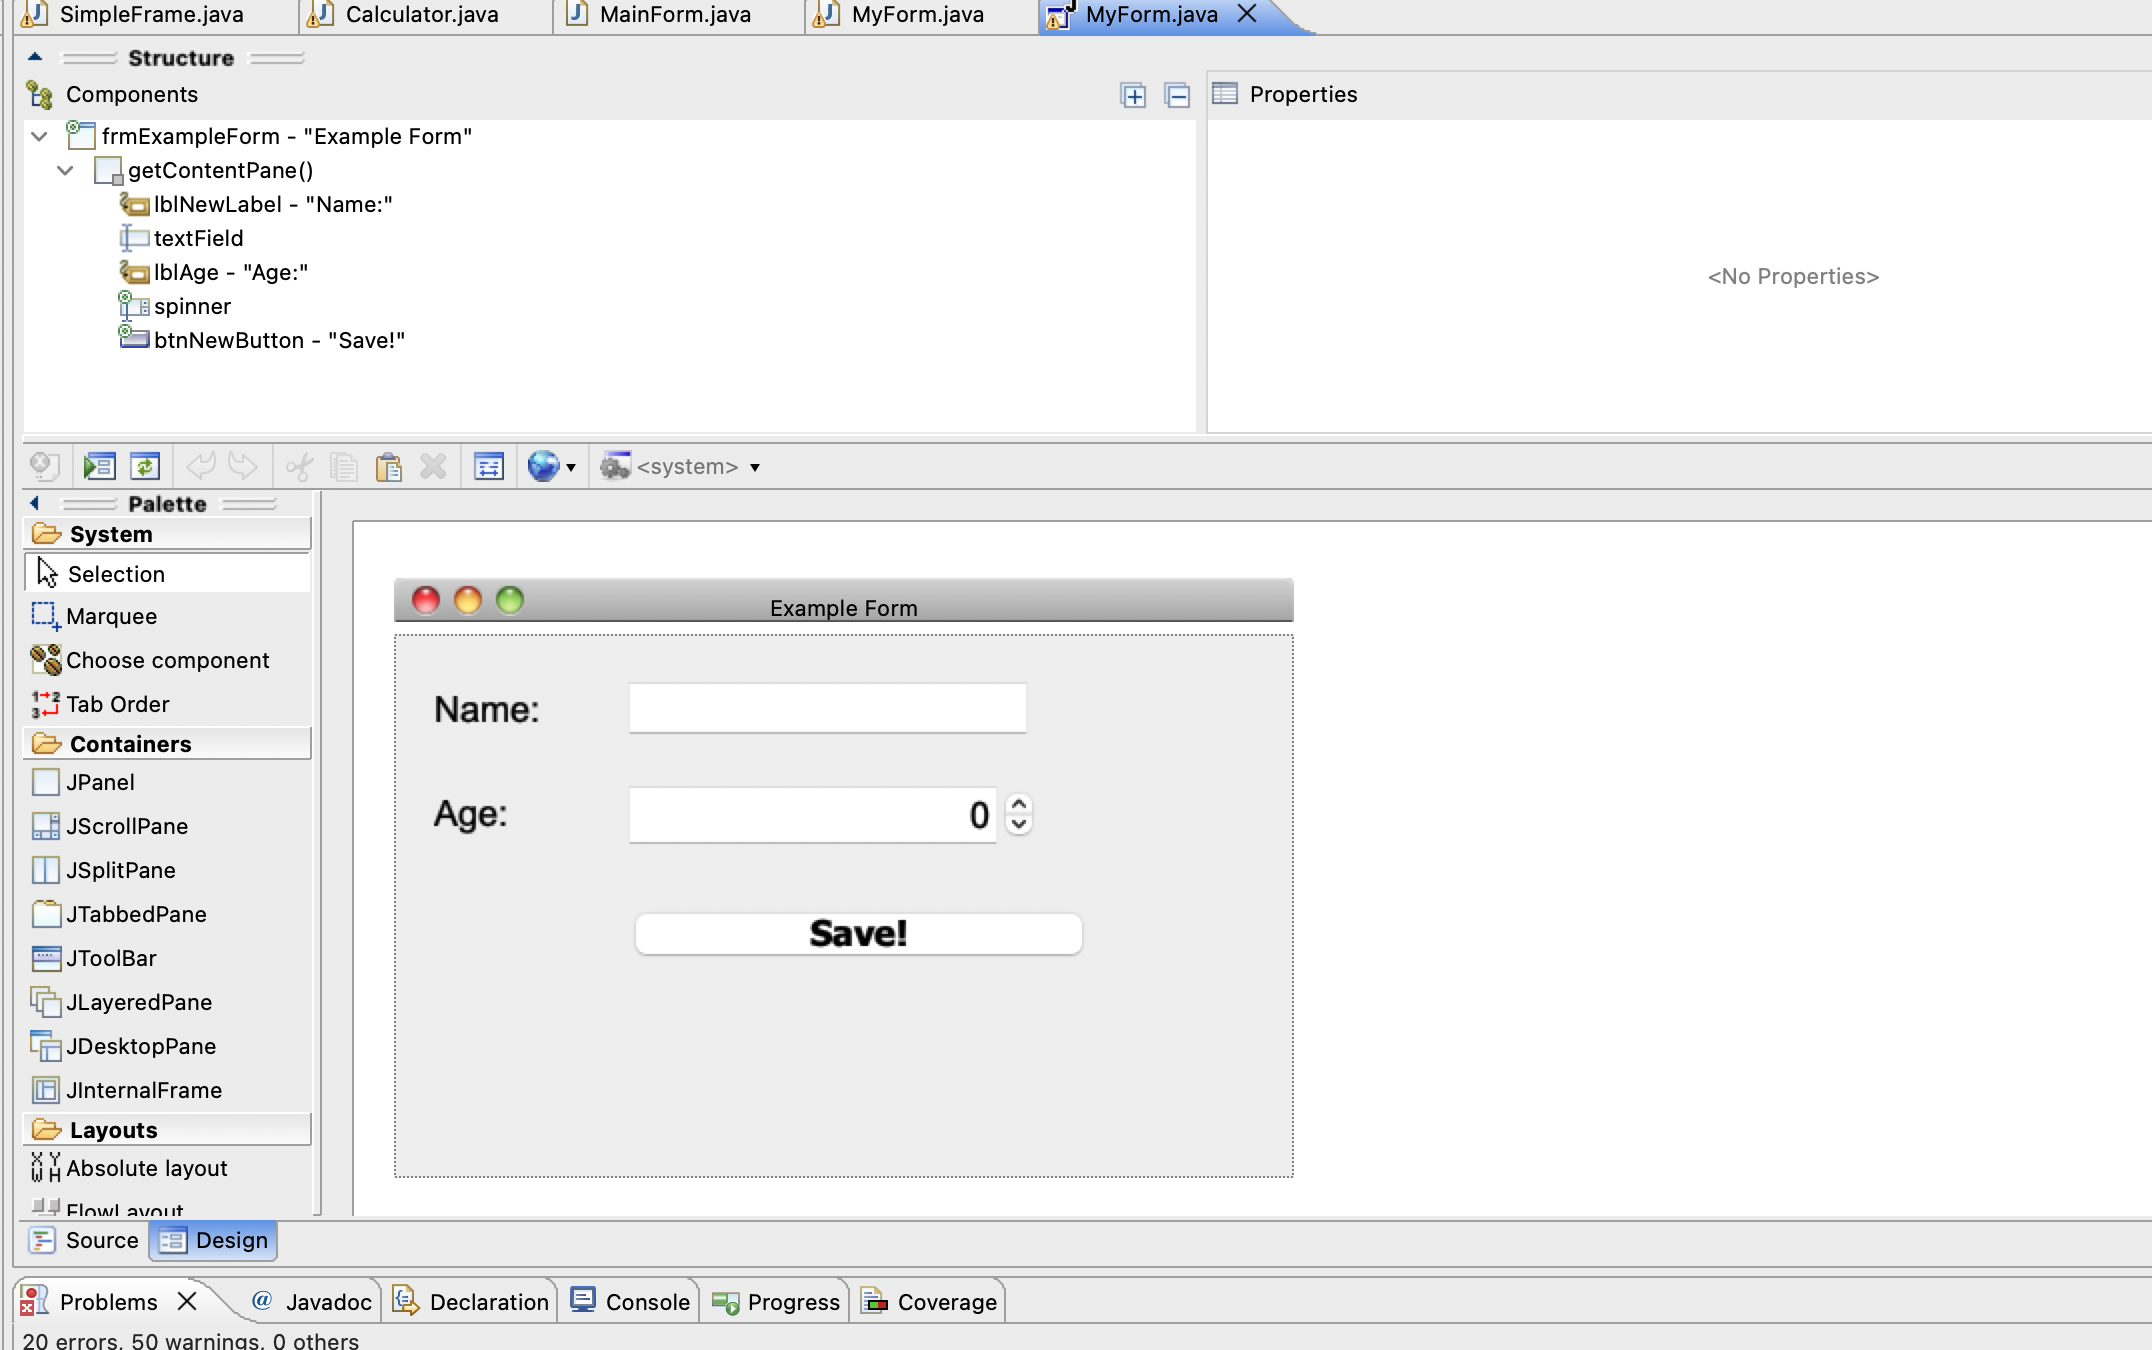
\includegraphics[width=0.8\textwidth]{assets/pertemuan11/myform_window_builder.png}
	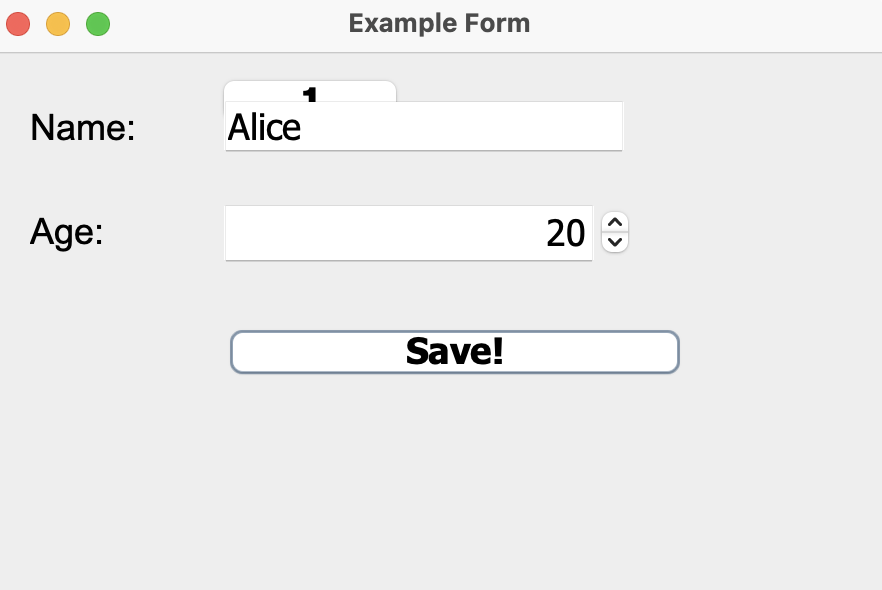
\includegraphics[width=0.8\textwidth]{assets/pertemuan11/myform.png}
	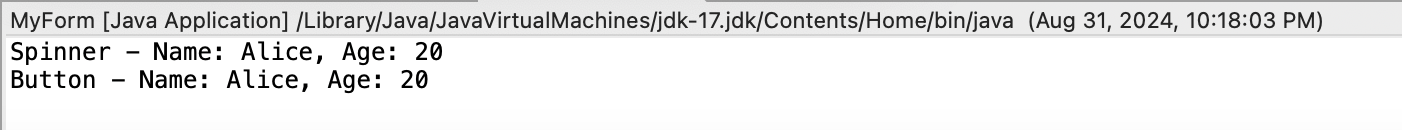
\includegraphics[width=0.8\textwidth]{assets/pertemuan11/myform_result.png}
\end{center}

\textbf{Kode Java:}
\begin{lstlisting}[style=JavaStyle]
	package edu.pradita.p11;
	
	import java.awt.EventQueue;
	import java.awt.Font;
	import java.awt.event.ActionEvent;
	import java.awt.event.ActionListener;
	import javax.swing.JButton;
	import javax.swing.JFrame;
	import javax.swing.JLabel;
	import javax.swing.JPanel;
	import javax.swing.JTextField;
	import javax.swing.JSpinner;
	import javax.swing.SpinnerNumberModel;
	
	public class MyForm extends JFrame {
		
		private JTextField nameField;
		private JSpinner ageSpinner;
		private JButton addButton;
		private JPanel panel;
		
		public MyForm() {
			initialize();
		}
		
		private void initialize() {
			setTitle("My Form");
			setBounds(100, 100, 450, 300);
			setDefaultCloseOperation(JFrame.EXIT_ON_CLOSE);
			panel = new JPanel();
			getContentPane().add(panel);
			panel.setLayout(null);
			
			JLabel nameLabel = new JLabel("Name:");
			nameLabel.setFont(new Font("Arial", Font.PLAIN, 14));
			nameLabel.setBounds(10, 20, 80, 25);
			panel.add(nameLabel);
			
			nameField = new JTextField();
			nameField.setBounds(100, 20, 165, 25);
			panel.add(nameField);
			
			JLabel ageLabel = new JLabel("Age:");
			ageLabel.setFont(new Font("Arial", Font.PLAIN, 14));
			ageLabel.setBounds(10, 50, 80, 25);
			panel.add(ageLabel);
			
			ageSpinner = new JSpinner(new SpinnerNumberModel(18, 0, 100, 1));
			ageSpinner.setBounds(100, 50, 50, 25);
			panel.add(ageSpinner);
			
			addButton = new JButton("Add");
			addButton.setBounds(10, 80, 80, 25);
			panel.add(addButton);
			
			addButton.addActionListener(new ActionListener() {
				@Override
				public void actionPerformed(ActionEvent e) {
					// Add action handling code here
				}
			});
			
			JButton addDynamicButton = new JButton("Add Dynamic Button");
			addDynamicButton.setBounds(10, 110, 200, 25);
			panel.add(addDynamicButton);
			
			addDynamicButton.addActionListener(new ActionListener() {
				@Override
				public void actionPerformed(ActionEvent e) {
					JButton dynamicButton = new JButton("Dynamic Button");
					dynamicButton.setBounds(10, 140 + (panel.getComponentCount() - 6) * 30, 200, 25);
					panel.add(dynamicButton);
					panel.revalidate();
					panel.repaint();
				}
			});
		}
		
		public static void main(String[] args) {
			EventQueue.invokeLater(new Runnable() {
				public void run() {
					try {
						MyForm frame = new MyForm();
						frame.setVisible(true);
					} catch (Exception e) {
						e.printStackTrace();
					}
				}
			});
		}
	}
\end{lstlisting}

\subsection{Kalkulator GUI}

\textbf{Kode:} \texttt{Calculator.java}

\textbf{Deskripsi:} Kode ini membuat aplikasi kalkulator sederhana menggunakan Swing di Java. Program ini terdiri dari beberapa komponen GUI seperti tombol angka, tombol operasi, dan layar tampilan.

\textbf{Penjelasan Kode:}
\begin{itemize}
	\item \texttt{Calculator} adalah kelas utama yang memperluas \texttt{JFrame} untuk membuat jendela GUI.
	\item \texttt{JPanel} digunakan untuk menyusun komponen dengan layout \texttt{BorderLayout} dan \texttt{GridLayout}.
	\item \texttt{JLabel} digunakan untuk menampilkan hasil kalkulasi.
	\item Tombol angka dibuat secara dinamis dalam sebuah loop dan ditambahkan ke panel tombol.
	\item Tombol \texttt{+} dan \texttt{=} ditambahkan untuk melakukan operasi penjumlahan dan menampilkan hasil.
	\item \texttt{calculate()} adalah metode untuk menghitung hasil operasi berdasarkan nilai yang disimpan dalam \texttt{accumulator}.
\end{itemize}

\textbf{Gambar:} \\
\begin{center}
	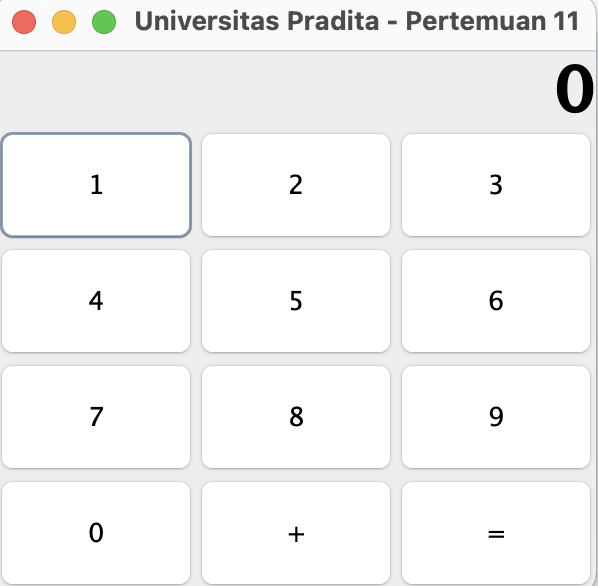
\includegraphics[width=0.5\textwidth]{assets/pertemuan11/calculator.png}
\end{center}

\textbf{Kode Java:}
\begin{lstlisting}[style=JavaStyle]
	package edu.pradita.p11;
	
	import java.awt.BorderLayout;
	import java.awt.Font;
	import java.awt.GridLayout;
	import java.awt.event.ActionEvent;
	import java.awt.event.ActionListener;
	import javax.swing.JButton;
	import javax.swing.JFrame;
	import javax.swing.JLabel;
	import javax.swing.JPanel;
	
	public class Calculator extends JFrame {
		
		private static final int FRAME_WIDTH = 300;
		private static final int FRAME_HEIGHT = 300;
		private static final int FONT_SIZE = 32;
		
		private Integer accumulator = null;
		private Integer value = 0;
		private String nextOperation = null;
		private boolean clearDisplay = false;
		
		public Calculator() {
			JPanel mainPanel = new JPanel();
			mainPanel.setLayout(new BorderLayout());
			this.add(mainPanel);
			
			JLabel display = new JLabel();
			display.setHorizontalAlignment(JLabel.RIGHT);
			display.setFont(new Font(display.getFont().getName(), Font.BOLD, 32));
			display.setText(String.valueOf(value));
			mainPanel.add(display, BorderLayout.NORTH);
			
			JPanel buttonPanel = new JPanel();
			buttonPanel.setLayout(new GridLayout(4, 3));
			mainPanel.add(buttonPanel, BorderLayout.CENTER);
			
			// Loop adding numeric button
			for (int i = 1; i <= 10; i++) {
				String valueText = (i < 10) ? valueText = String.valueOf(i) : "0";
				JButton button = new JButton();
				button.setText(valueText);
				buttonPanel.add(button);
				
				ActionListener numericButtonListener = new ActionListener() {
					@Override
					public void actionPerformed(ActionEvent e) {
						if (display.getText().equals("0")) {
							display.setText("" + button.getText());
						} else {
							if (clearDisplay) {
								display.setText("");
								clearDisplay = false;
							}
							display.setText(display.getText() + button.getText());
						}
						value = Integer.valueOf(display.getText());
					}
				};
				button.addActionListener(numericButtonListener);
			}
			
			// adding add button
			JButton button = new JButton();
			button.setText("+");
			buttonPanel.add(button);
			
			ActionListener addButtonListener = new ActionListener() {
				@Override
				public void actionPerformed(ActionEvent e) {
					nextOperation = "+";
					if (accumulator == null) {
						accumulator = Integer.valueOf(display.getText());
					} else {
						calculate();
						display.setText(String.valueOf(accumulator));
					}
					value = 0;
					clearDisplay = true;
				}
			};
			button.addActionListener(addButtonListener);
			
			// adding equal button
			JButton equalButton = new JButton();
			equalButton.setText("=");
			buttonPanel.add(equalButton);
			
			ActionListener equalButtonListener = new ActionListener() {
				@Override
				public void actionPerformed(ActionEvent e) {
					if (accumulator != null && nextOperation != null) {
						calculate();
						display.setText(String.valueOf(accumulator));
					}
					clearDisplay = true;
				}
			};
			equalButton.addActionListener(equalButtonListener);
			
			setSize(FRAME_WIDTH, FRAME_HEIGHT);
		}
		
		public void calculate() {
			if (nextOperation == "+") {
				accumulator = accumulator + value;
			}
		}
	}
\end{lstlisting}






\subsection{Main Form}

\textbf{Kode:} \texttt{MainForm.java}

\textbf{Deskripsi:} Kode ini membuat dua jendela GUI: satu untuk \texttt{SimpleFrame} dan satu untuk \texttt{Calculator}. \texttt{MainForm} adalah kelas utama yang menjalankan aplikasi dan menampilkan kedua jendela.

\textbf{Penjelasan Kode:}
\begin{itemize}
	\item \texttt{MainForm} adalah kelas utama dengan metode \texttt{main} yang membuat dan menampilkan jendela \texttt{SimpleFrame} dan \texttt{Calculator}.
	\item \texttt{frame.setLocationRelativeTo(null)} memastikan jendela ditempatkan di pusat layar.
	\item \texttt{setTitle}, \texttt{setDefaultCloseOperation}, dan \texttt{setVisible} digunakan untuk mengatur judul, operasi penutupan, dan visibilitas jendela.
\end{itemize}

\textbf{Gambar:} \\
\begin{center}
	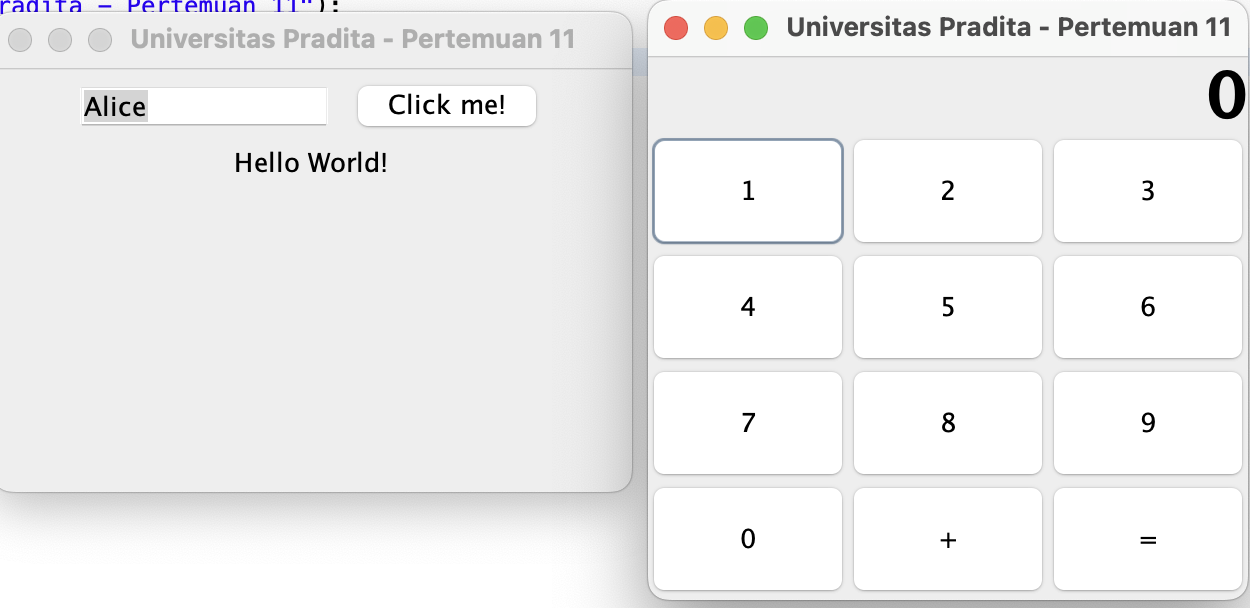
\includegraphics[width=0.8\textwidth]{assets/pertemuan11/main_form.png}
\end{center}

\textbf{Kode Java:}
\begin{lstlisting}[style=JavaStyle]
	package edu.pradita.p11;
	
	import javax.swing.JFrame;
	
	public class MainForm {
		public static void main(String[] args) {
			JFrame frame = new SimpleFrame();
			frame.setLocationRelativeTo(null); // put the frame at the centre
			frame.setTitle("Universitas Pradita - Pertemuan 11");
			frame.setDefaultCloseOperation(JFrame.EXIT_ON_CLOSE);
			frame.setVisible(true);
			
			JFrame calculator = new Calculator();
			calculator.setLocationRelativeTo(null); // put the frame at the centre
			calculator.setTitle("Universitas Pradita - Pertemuan 11");
			calculator.setDefaultCloseOperation(JFrame.EXIT_ON_CLOSE);
			calculator.setVisible(true);
		}
	}
\end{lstlisting}


\section{Latihan dan Contoh Kode: BMI Calculator}

Pada latihan ini, Anda akan membuat aplikasi GUI untuk menghitung Body Mass Index (BMI). Aplikasi ini harus memiliki inputan untuk berat badan (dalam kilogram) dan tinggi badan (dalam meter). Setelah pengguna memasukkan data dan menekan tombol “Hitung”, BMI akan ditampilkan di layar.

\textbf{Instruksi:}
\begin{enumerate}
	\item Buatlah GUI menggunakan WindowBuilder di Eclipse.
	\item Buatlah inputan untuk berat badan (dalam kilogram) dan tinggi badan (dalam meter).
	\item Tambahkan tombol “Hitung” yang akan menghitung BMI berdasarkan inputan pengguna.
	\item Tampilkan hasil BMI setelah tombol ditekan.
\end{enumerate}


\textbf{Gambar:} \\
\begin{center}
	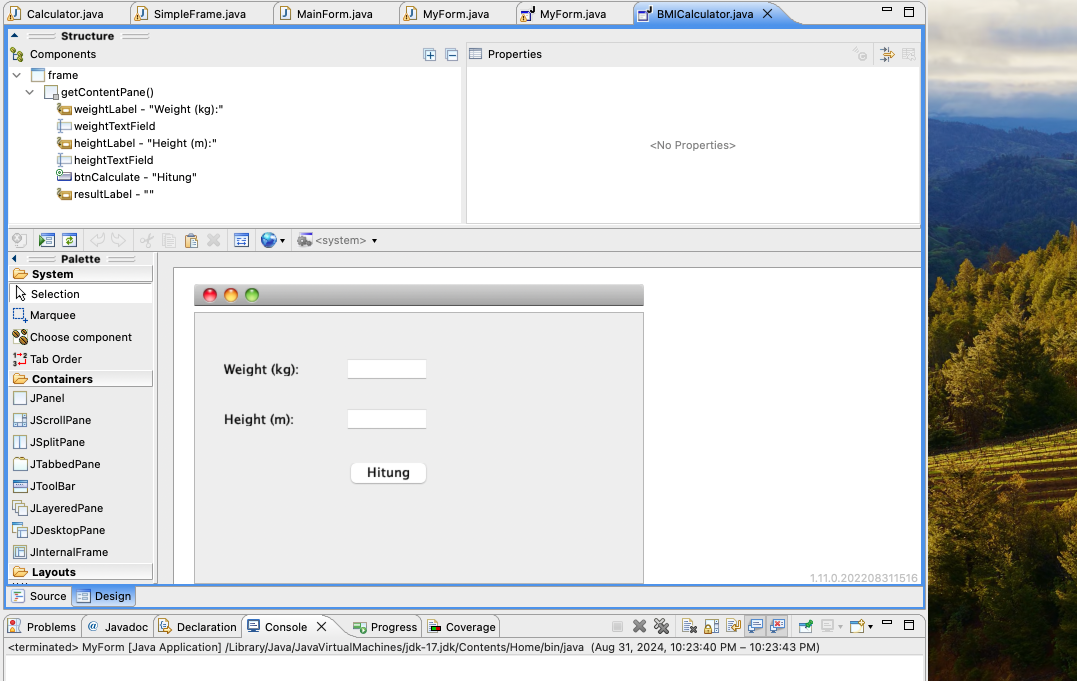
\includegraphics[width=0.8\textwidth]{assets/pertemuan11/bmicalculator_window_builder.png}
	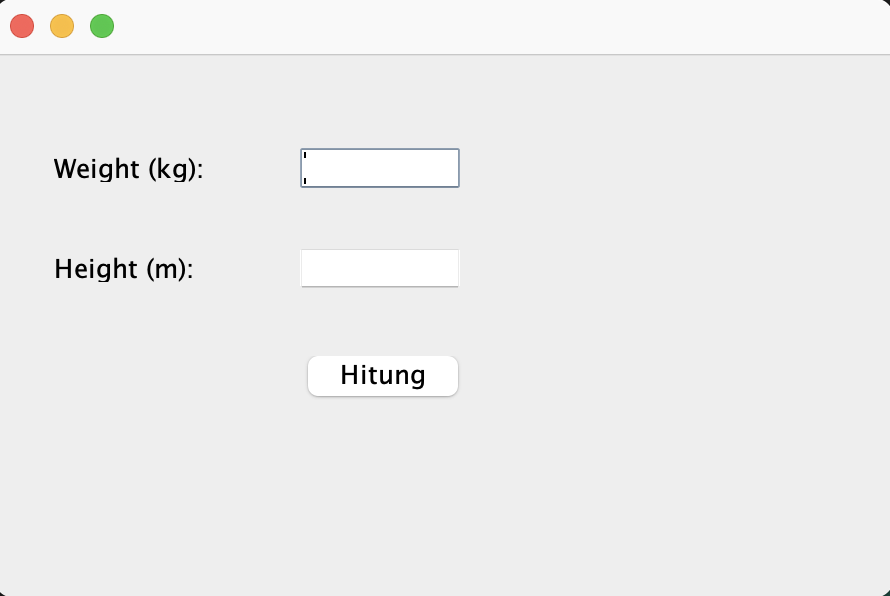
\includegraphics[width=0.8\textwidth]{assets/pertemuan11/bmicalculator.png}
\end{center}


\textbf{Kode Java:}

\begin{lstlisting}[style=JavaStyle]
	import java.awt.EventQueue;
	import javax.swing.JFrame;
	import javax.swing.JLabel;
	import javax.swing.JTextField;
	import javax.swing.JButton;
	import java.awt.event.ActionListener;
	import java.awt.event.ActionEvent;
	
	public class BMICalculator {
		
		private JFrame frame;
		private JTextField weightTextField;
		private JTextField heightTextField;
		private JLabel resultLabel;
		
		/**
		* Launch the application.
		*/
		public static void main(String[] args) {
			EventQueue.invokeLater(new Runnable() {
				public void run() {
					try {
						BMICalculator window = new BMICalculator();
						window.frame.setVisible(true);
					} catch (Exception e) {
						e.printStackTrace();
					}
				}
			});
		}
		
		/**
		* Create the application.
		*/
		public BMICalculator() {
			initialize();
		}
		
		/**
		* Initialize the contents of the frame.
		*/
		private void initialize() {
			frame = new JFrame();
			frame.setBounds(100, 100, 450, 300);
			frame.setDefaultCloseOperation(JFrame.EXIT_ON_CLOSE);
			frame.getContentPane().setLayout(null);
			
			JLabel weightLabel = new JLabel("Weight (kg):");
			weightLabel.setBounds(30, 50, 100, 14);
			frame.getContentPane().add(weightLabel);
			
			weightTextField = new JTextField();
			weightTextField.setBounds(150, 47, 86, 20);
			frame.getContentPane().add(weightTextField);
			weightTextField.setColumns(10);
			
			JLabel heightLabel = new JLabel("Height (m):");
			heightLabel.setBounds(30, 100, 100, 14);
			frame.getContentPane().add(heightLabel);
			
			heightTextField = new JTextField();
			heightTextField.setBounds(150, 97, 86, 20);
			frame.getContentPane().add(heightTextField);
			heightTextField.setColumns(10);
			
			JButton btnCalculate = new JButton("Hitung");
			btnCalculate.addActionListener(new ActionListener() {
				public void actionPerformed(ActionEvent e) {
					double weight = Double.parseDouble(weightTextField.getText());
					double height = Double.parseDouble(heightTextField.getText());
					double bmi = weight / (height * height);
					resultLabel.setText(String.format("Your BMI is: %.2f", bmi));
				}
			});
			btnCalculate.setBounds(150, 150, 89, 23);
			frame.getContentPane().add(btnCalculate);
			
			resultLabel = new JLabel("");
			resultLabel.setBounds(150, 200, 200, 14);
			frame.getContentPane().add(resultLabel);
		}
	}
\end{lstlisting}


\section{Soal}

Berikut adalah instruksi untuk dua proyek yang akan membantu memahami penggunaan \textit{Java Swing} dalam membangun aplikasi sederhana.

\subsection*{Proyek 1: Permainan Tic-Tac-Toe}
\textbf{Tujuan}: Mengembangkan permainan Tic-Tac-Toe interaktif sederhana menggunakan Java Swing untuk dua pemain.

\textbf{Instruksi}:
\begin{enumerate}
	\item \textbf{Atur GUI}:
	\begin{itemize}
		\item Buat papan permainan 3x3 menggunakan \texttt{JPanel} dengan \texttt{GridLayout} untuk papan Tic-Tac-Toe.
		\item Tambahkan sembilan \texttt{JButton} dalam grid untuk mewakili kotak-kotak tempat pemain akan menempatkan simbol mereka (X atau O).
	\end{itemize}
	
	\item \textbf{Logika Permainan}:
	\begin{itemize}
		\item Terapkan logika pergantian giliran agar permainan bergiliran antara dua pemain (Pemain X dan Pemain O).
		\item Gunakan variabel internal, seperti \texttt{boolean isXTurn}, untuk melacak giliran siapa saat ini. Inisialisasi dengan \texttt{true} (giliran Pemain X).
	\end{itemize}
	
	\item \textbf{Aksi Klik Tombol}:
	\begin{itemize}
		\item Tambahkan \texttt{ActionListener} ke masing-masing tombol. Ketika pemain mengklik tombol, periksa apakah kotak kosong.
		\item Jika kosong, perbarui tombol dengan simbol pemain saat ini (X atau O), lalu ubah giliran dengan memperbarui \texttt{isXTurn}.
		\item Nonaktifkan tombol setelah diklik untuk mencegah perubahan lebih lanjut.
	\end{itemize}
	
	\item \textbf{Menentukan Pemenang}:
	\begin{itemize}
		\item Periksa pemenang setelah setiap gerakan dengan memeriksa label tombol di setiap baris, kolom, dan diagonal.
		\item Jika seorang pemain memiliki tiga simbol berturut-turut, tampilkan dialog pesan (misalnya, \texttt{JOptionPane.showMessageDialog}) yang menyatakan pemenang.
		\item Jika semua kotak terisi tanpa pemenang, tampilkan pesan yang menyatakan seri.
	\end{itemize}
	
	\item \textbf{Opsi Reset}:
	\begin{itemize}
		\item Tambahkan tombol "Permainan Baru" atau "Reset" untuk memulai permainan baru.
		\item Atur ulang semua tombol menjadi kosong dan aktifkan kembali untuk permainan baru. Set \texttt{isXTurn} kembali ke \texttt{true} untuk memulai dengan Pemain X.
	\end{itemize}
	
	\item \textbf{Penanganan Kesalahan}:
	\begin{itemize}
		\item Pastikan tindakan tidak valid dicegah, seperti mengklik kotak yang sudah berisi simbol.
		\item Tangani setiap pengecualian secara tepat, memberikan umpan balik yang bermanfaat jika diperlukan.
	\end{itemize}
\end{enumerate}

\textbf{Hasil Akhir}: Program permainan Tic-Tac-Toe yang berfungsi, bergiliran, memeriksa pemenang atau seri, dan dapat diatur ulang.

\subsection*{Proyek 2: Aplikasi Daftar Tugas}
\textbf{Tujuan}: Membangun aplikasi Daftar Tugas yang memungkinkan pengguna menambah, menandai, dan menghapus tugas.

\textbf{Instruksi}:
\begin{enumerate}
	\item \textbf{Atur GUI}:
	\begin{itemize}
		\item Buat \texttt{JFrame} utama untuk jendela aplikasi.
		\item Tambahkan \texttt{JTextField} di bagian atas untuk mengetik tugas yang ingin ditambahkan.
		\item Tambahkan tombol "Tambahkan Tugas" di samping kolom teks untuk menambah tugas ke daftar.
		\item Gunakan komponen \texttt{JList} untuk menampilkan daftar tugas. Atur model daftar dengan menggunakan (\texttt{DefaultListModel<String>}) untuk menambah dan menghapus tugas secara dinamis.
	\end{itemize}
	
	\item \textbf{Menambah Tugas}:
	\begin{itemize}
		\item Ketika pengguna mengetik tugas dan menekan tombol "Tambahkan Tugas", tambahkan tugas ke dalam \texttt{JList}.
		\item Kosongkan kolom teks setelah menambahkan tugas untuk memudahkan penambahan berikutnya.
	\end{itemize}
	
	\item \textbf{Menandai Tugas sebagai Selesai}:
	\begin{itemize}
		\item Tambahkan tombol "Tandai Selesai" yang memungkinkan pengguna menandai tugas yang dipilih sebagai selesai.
		\item Ketika pengguna memilih tugas di \texttt{JList} dan menekan "Tandai Selesai", perbarui tampilan tugas (misalnya, tambahkan tanda "(Selesai)" atau ubah warnanya).
	\end{itemize}
	
	\item \textbf{Menghapus Tugas}:
	\begin{itemize}
		\item Tambahkan tombol "Hapus Tugas" yang menghapus tugas yang dipilih dari daftar ketika diklik.
		\item Konfirmasi penghapusan dengan dialog (\texttt{JOptionPane.showConfirmDialog}) untuk mencegah penghapusan tidak sengaja.
	\end{itemize}
	
	\item \textbf{Opsi Hapus Semua}:
	\begin{itemize}
		\item Secara opsional, tambahkan tombol "Hapus Semua" yang menghapus semua tugas dari daftar setelah konfirmasi dari pengguna.
	\end{itemize}
	
	\item \textbf{Penanganan Kesalahan}:
	\begin{itemize}
		\item Pastikan tindakan seperti menandai atau menghapus hanya memengaruhi tugas saat satu tugas dipilih. Tampilkan pesan kesalahan jika tidak ada tugas yang dipilih.
	\end{itemize}
\end{enumerate}

\textbf{Hasil Akhir}: Program Aplikasi Daftar Tugas yang dapat menambah, menandai selesai, dan menghapus tugas dengan tampilan yang jelas dan mudah digunakan.




	\chapter{GUI dan File Input Output}

\section{GUI dan File Input Output di Java}

\subsection{Swing dan GUI di Java}

Swing adalah toolkit GUI (Graphical User Interface) dalam Java yang memungkinkan pembuatan aplikasi desktop dengan antarmuka grafis. Berikut adalah beberapa komponen Swing yang digunakan dalam kode:

\begin{itemize}
	\item \texttt{JFrame}: Komponen utama yang menyimpan dan menampilkan elemen-elemen GUI lainnya dalam sebuah jendela. Di kode ini, \texttt{JFrame} digunakan untuk menampilkan jendela login (\texttt{LoginForm}) dan formulir tambah pengguna (\texttt{AddUserForm}).
	\begin{lstlisting}[style=JavaStyle]
		frmLoginScreen = new JFrame();
	\end{lstlisting}
	
	\item \texttt{JPanel}: Kontainer yang digunakan untuk menyusun dan mengatur tata letak komponen GUI lainnya. Dalam \texttt{AddUserForm}, \texttt{JPanel} digunakan untuk menampung label, field input, dan tombol.
	\begin{lstlisting}[style=JavaStyle]
		contentPane = new JPanel();
	\end{lstlisting}
	
	\item \texttt{JButton}: Komponen yang dapat diklik oleh pengguna untuk melakukan aksi tertentu. Dalam kode, tombol ini digunakan untuk login dan menambah pengguna.
	\begin{lstlisting}[style=JavaStyle]
		JButton btnNewButton = new JButton("Login");
	\end{lstlisting}
	
	\item \texttt{JTextField}: Komponen input teks yang memungkinkan pengguna untuk memasukkan data. Digunakan untuk nama pengguna dan kata sandi.
	\begin{lstlisting}[style=JavaStyle]
		JTextField txtUsername = new JTextField();
	\end{lstlisting}
	
	\item \texttt{JTable}: Komponen yang menampilkan data dalam format tabel. Digunakan dalam \texttt{AddUserForm} untuk menampilkan daftar pengguna yang telah ditambahkan.
	\begin{lstlisting}[style=JavaStyle]
		usersTable = new JTable();
	\end{lstlisting}
\end{itemize}

\subsection{Pengelolaan File dan I/O di Java}

Pengelolaan file dan I/O (Input/Output) di Java digunakan untuk membaca dari dan menulis ke file. Dalam kode ini, digunakan untuk menyimpan dan memuat data pengguna ke dalam file CSV.

\begin{itemize}
	\item \texttt{File}: Kelas yang mewakili file atau direktori di sistem file. Digunakan untuk menentukan lokasi file yang akan dibaca atau ditulis.
	\begin{lstlisting}[style=JavaStyle]
		File file = new File("data.csv");
	\end{lstlisting}
	
	\item \texttt{FileReader}: Kelas yang digunakan untuk membaca data karakter dari file.
	\begin{lstlisting}[style=JavaStyle]
		FileReader fr = new FileReader(file);
	\end{lstlisting}
	
	\item \texttt{FileWriter}: Kelas yang digunakan untuk menulis data karakter ke file.
	\begin{lstlisting}[style=JavaStyle]
		FileWriter fw = new FileWriter(file);
	\end{lstlisting}
	
	\item \texttt{BufferedReader}: Kelas yang membungkus \texttt{FileReader} untuk meningkatkan efisiensi pembacaan dengan menggunakan buffer.
	\begin{lstlisting}[style=JavaStyle]
		BufferedReader br = new BufferedReader(fr);
	\end{lstlisting}
	
	\item \texttt{BufferedWriter}: Kelas yang membungkus \texttt{FileWriter} untuk meningkatkan efisiensi penulisan dengan menggunakan buffer.
	\begin{lstlisting}[style=JavaStyle]
		BufferedWriter bw = new BufferedWriter(fw);
	\end{lstlisting}
\end{itemize}

\subsection{Penanganan Aksi dan Event di Java}

Penanganan aksi dan event memungkinkan aplikasi untuk merespons interaksi pengguna, seperti klik tombol.

\begin{itemize}
	\item \texttt{ActionListener}: Antarmuka yang harus diimplementasikan untuk menangani peristiwa aksi, seperti klik tombol.
	\begin{lstlisting}[style=JavaStyle]
		btnNewButton.addActionListener(new ActionListener() {
			public void actionPerformed(ActionEvent e) {
				// Kode untuk menangani klik tombol
			}
		});
	\end{lstlisting}
\end{itemize}




\section{Penjelasan Kode Java dengan GUI}

Kode Java berikut adalah implementasi sederhana dari sistem manajemen pengguna dengan antarmuka grafis pengguna (GUI) menggunakan Swing. Sistem ini terdiri dari tiga kelas utama: \texttt{User}, \texttt{Data}, dan \texttt{LoginForm}. Berikut adalah penjelasan dari setiap kelas dan fungsinya.

\subsection{Kelas \texttt{User}}

\textbf{Deskripsi:} Kelas \texttt{User} mewakili entitas pengguna dengan atribut \texttt{username} dan \texttt{password}.

\begin{lstlisting}[style=JavaStyle]
	package edu.pradita.p10;
	
	public class User {
		
		private String username;
		private String password;
		
		public User(String username, String password) {
			this.username = username;
			this.password = password;
		}
		
		public String getUsername() {
			return username;
		}
		
		public void setUsername(String username) {
			this.username = username;
		}
		
		public String getPassword() {
			return password;
		}
		
		public void setPassword(String password) {
			this.password = password;
		}
	}
\end{lstlisting}

\textbf{Keterangan:} 
\begin{itemize}
	\item \texttt{User(String username, String password)}: Konstruktor untuk menginisialisasi objek \texttt{User}.
	\item \texttt{getUsername()}: Mengambil nama pengguna.
	\item \texttt{setUsername(String username)}: Mengatur nama pengguna.
	\item \texttt{getPassword()}: Mengambil kata sandi.
	\item \texttt{setPassword(String password)}: Mengatur kata sandi.
\end{itemize}

\subsection{Kelas \texttt{Data}}

\textbf{Deskripsi:} Kelas \texttt{Data} menangani penyimpanan dan pemuatan data pengguna dari dan ke file CSV.

\begin{lstlisting}[style=JavaStyle]
	package edu.pradita.p10;
	
	import java.io.BufferedReader;
	import java.io.BufferedWriter;
	import java.io.File;
	import java.io.FileReader;
	import java.io.FileWriter;
	import java.io.IOException;
	import java.util.ArrayList;
	import java.util.List;
	
	public class Data {
		
		private static List<User> users = new ArrayList<>();
		
		public static List<User> getUsers() {
			return users;
		}
		
		public static List<User> saveUsers(List<User> users) {
			try {
				Data.users.clear();
				Data.users.addAll(users);
				
				File file = new File("data.csv");
				FileWriter fw = new FileWriter(file);
				BufferedWriter bw = new BufferedWriter(fw);
				
				for (User user : Data.users) {
					bw.write(user.getUsername() + "," + user.getPassword() + System.lineSeparator());
				}
				
				bw.close();
			} catch (IOException e) {
				e.printStackTrace();
			}
			
			return users;
		}
		
		public static List<User> loadUsers() {
			try {
				File file = new File("data.csv");
				FileReader fr = new FileReader(file);
				BufferedReader br = new BufferedReader(fr);
				
				String line = br.readLine();
				while (line != null) {
					String[] lineArray = line.split(",");
					users.add(new User(lineArray[0].trim(), lineArray[1].trim()));
					line = br.readLine();
				}
				br.close();
			} catch (IOException e) {
				e.printStackTrace();
			}
			
			return users;
		}
	}
\end{lstlisting}

\textbf{Keterangan:} 
\begin{itemize}
	\item \texttt{saveUsers(List<User> users)}: Menyimpan daftar pengguna ke file CSV.
	\item \texttt{loadUsers()}: Memuat daftar pengguna dari file CSV.
\end{itemize}

\subsection{Kelas \texttt{LoginForm}}

\textbf{Deskripsi:} Kelas \texttt{LoginForm} menyediakan antarmuka pengguna untuk login. Setelah login berhasil, pengguna diarahkan ke formulir \texttt{AddUserForm}.

\begin{lstlisting}[style=JavaStyle]
	package edu.pradita.p10;
	
	import java.awt.Dialog.ModalityType;
	import java.awt.EventQueue;
	import java.awt.FlowLayout;
	import java.awt.Font;
	import java.awt.GraphicsEnvironment;
	import java.awt.Point;
	import java.awt.event.ActionEvent;
	import java.awt.event.ActionListener;
	import java.util.List;
	
	import javax.swing.JButton;
	import javax.swing.JDialog;
	import javax.swing.JFrame;
	import javax.swing.JLabel;
	import javax.swing.JPasswordField;
	import javax.swing.JTextField;
	
	public class LoginForm {
		
		private JFrame frmLoginScreen;
		private JPasswordField txtPassword;
		private static List<User> users = Data.loadUsers();
		
		public static void main(String[] args) {
			EventQueue.invokeLater(new Runnable() {
				public void run() {
					try {
						LoginForm window = new LoginForm();
						window.frmLoginScreen.setVisible(true);
					} catch (Exception e) {
						e.printStackTrace();
					}
				}
			});
		}
		
		public LoginForm() {
			initialize();
		}
		
		private void initialize() {
			frmLoginScreen = new JFrame();
			frmLoginScreen.getContentPane().setFont(new Font("Tahoma", Font.PLAIN, 18));
			frmLoginScreen.setTitle("Login Screen");
			frmLoginScreen.setSize(400, 300);
			frmLoginScreen.setDefaultCloseOperation(JFrame.EXIT_ON_CLOSE);
			frmLoginScreen.getContentPane().setLayout(null);
			Point centerPoint = GraphicsEnvironment.getLocalGraphicsEnvironment().getCenterPoint();
			frmLoginScreen.setLocation(centerPoint.x - (int) frmLoginScreen.getSize().getWidth() / 2,
			centerPoint.y - (int) frmLoginScreen.getSize().getHeight() / 2);
			
			JLabel lblUsername = new JLabel("Username");
			lblUsername.setFont(new Font("Tahoma", Font.PLAIN, 16));
			lblUsername.setBounds(92, 88, 96, 19);
			frmLoginScreen.getContentPane().add(lblUsername);
			
			JTextField txtUsername = new JTextField();
			txtUsername.setFont(new Font("Tahoma", Font.PLAIN, 16));
			txtUsername.setBounds(197, 87, 107, 19);
			frmLoginScreen.getContentPane().add(txtUsername);
			txtUsername.setColumns(10);
			
			txtPassword = new JPasswordField();
			txtPassword.setFont(new Font("Tahoma", Font.PLAIN, 16));
			txtPassword.setBounds(197, 116, 107, 19);
			frmLoginScreen.getContentPane().add(txtPassword);
			
			JLabel lblPassword = new JLabel("Password");
			lblPassword.setFont(new Font("Tahoma", Font.PLAIN, 16));
			lblPassword.setBounds(92, 117, 96, 19);
			frmLoginScreen.getContentPane().add(lblPassword);
			
			JButton btnNewButton = new JButton("Login");
			btnNewButton.addActionListener(new ActionListener() {
				public void actionPerformed(ActionEvent e) {
					
					String username = txtUsername.getText();
					String password = String.valueOf(txtPassword.getPassword());
					
					for (User user : users) {
						if (user.getUsername().equals(username) && user.getPassword().equals(password)) {
							AddUserForm addUserForm = new AddUserForm();
							addUserForm.setVisible(true);
							addUserForm.setTitle("Current User: " + user.getUsername());
							frmLoginScreen.setVisible(false);
							return;
						}
					}
					JDialog dialog = new JDialog(frmLoginScreen, "Message", ModalityType.APPLICATION_MODAL);
					JLabel label = new JLabel("Your data is not found!");
					dialog.setLayout(new FlowLayout());
					dialog.add(label);
					dialog.setLocationRelativeTo(frmLoginScreen);
					dialog.setSize(150, 100);
					dialog.setVisible(true);
				}
			});
			btnNewButton.setFont(new Font("Tahoma", Font.PLAIN, 16));
			btnNewButton.setBounds(197, 145, 85, 21);
			frmLoginScreen.getContentPane().add(btnNewButton);
		}
	}
\end{lstlisting}

\textbf{Keterangan:} 
\begin{itemize}
	\item \texttt{initialize()}: Mengatur tampilan GUI untuk login.
	\item \texttt{btnNewButton.addActionListener()}: Menangani klik tombol login, memvalidasi pengguna, dan menampilkan \texttt{AddUserForm} jika login berhasil.
\end{itemize}

\subsection{Kelas \texttt{AddUserForm}}

\textbf{Deskripsi:} Kelas \texttt{AddUserForm} menyediakan antarmuka pengguna untuk menambah atau memperbarui data pengguna. Data pengguna ditampilkan dalam tabel yang dapat diedit.

\begin{lstlisting}[style=JavaStyle]
	package edu.pradita.p10;
	
	import java.awt.Dialog.ModalityType;
	import java.awt.EventQueue;
	import java.awt.FlowLayout;
	import java.awt.Font;
	import java.awt.GraphicsEnvironment;
	import java.awt.Point;
	import java.awt.event.ActionEvent;
	import java.awt.event.ActionListener;
	import java.util.ArrayList;
	import java.util.List;
	
	import javax.swing.JButton;
	import javax.swing.JDialog;
	import javax.swing.JFrame;
	import javax.swing.JLabel;
	import javax.swing.JPanel;
	import javax.swing.JScrollPane;
	import javax.swing.JTable;
	import javax.swing.JTextField;
	import javax.swing.table.DefaultTableModel;
	
	public class AddUserForm {
		
		private JFrame frmAddUserForm;
		private JTextField txtUsername;
		private JTextField txtPassword;
		private static List<User> users = Data.getUsers();
		private static DefaultTableModel model;
		
		public static void main(String[] args) {
			EventQueue.invokeLater(new Runnable() {
				public void run() {
					try {
						AddUserForm window = new AddUserForm();
						window.frmAddUserForm.setVisible(true);
					} catch (Exception e) {
						e.printStackTrace();
					}
				}
			});
		}
		
		public AddUserForm() {
			initialize();
		}
		
		private void initialize() {
			frmAddUserForm = new JFrame();
			frmAddUserForm.setTitle("Add User Form");
			frmAddUserForm.setBounds(100, 100, 450, 300);
			frmAddUserForm.setDefaultCloseOperation(JFrame.DISPOSE_ON_CLOSE);
			frmAddUserForm.getContentPane().setLayout(null);
			Point centerPoint = GraphicsEnvironment.getLocalGraphicsEnvironment().getCenterPoint();
			frmAddUserForm.setLocation(centerPoint.x - (int) frmAddUserForm.getSize().getWidth() / 2,
			centerPoint.y - (int) frmAddUserForm.getSize().getHeight() / 2);
			
			JPanel panel = new JPanel();
			panel.setBounds(12, 12, 408, 174);
			frmAddUserForm.getContentPane().add(panel);
			panel.setLayout(null);
			
			JLabel lblUsername = new JLabel("Username");
			lblUsername.setFont(new Font("Tahoma", Font.PLAIN, 16));
			lblUsername.setBounds(12, 12, 96, 19);
			panel.add(lblUsername);
			
			txtUsername = new JTextField();
			txtUsername.setFont(new Font("Tahoma", Font.PLAIN, 16));
			txtUsername.setBounds(120, 12, 274, 19);
			panel.add(txtUsername);
			txtUsername.setColumns(10);
			
			JLabel lblPassword = new JLabel("Password");
			lblPassword.setFont(new Font("Tahoma", Font.PLAIN, 16));
			lblPassword.setBounds(12, 41, 96, 19);
			panel.add(lblPassword);
			
			txtPassword = new JTextField();
			txtPassword.setFont(new Font("Tahoma", Font.PLAIN, 16));
			txtPassword.setBounds(120, 41, 274, 19);
			panel.add(txtPassword);
			txtPassword.setColumns(10);
			
			JButton btnAddUser = new JButton("Add User");
			btnAddUser.addActionListener(new ActionListener() {
				public void actionPerformed(ActionEvent e) {
					String username = txtUsername.getText();
					String password = txtPassword.getText();
					User user = new User(username, password);
					users.add(user);
					Data.saveUsers(users);
					
					model.setRowCount(0);
					for (User u : users) {
						model.addRow(new Object[] { u.getUsername(), u.getPassword() });
					}
					
					txtUsername.setText("");
					txtPassword.setText("");
				}
			});
			btnAddUser.setFont(new Font("Tahoma", Font.PLAIN, 16));
			btnAddUser.setBounds(298, 70, 96, 25);
			panel.add(btnAddUser);
			
			JScrollPane scrollPane = new JScrollPane();
			scrollPane.setBounds(12, 87, 382, 75);
			panel.add(scrollPane);
			
			JTable table = new JTable();
			model = new DefaultTableModel();
			model.addColumn("Username");
			model.addColumn("Password");
			table.setModel(model);
			scrollPane.setViewportView(table);
			
			for (User u : users) {
				model.addRow(new Object[] { u.getUsername(), u.getPassword() });
			}
		}
	}
\end{lstlisting}

\textbf{Keterangan:} 
\begin{itemize}
	\item \texttt{initialize()}: Mengatur tampilan GUI untuk menambah pengguna.
	\item \texttt{btnAddUser.addActionListener()}: Menangani klik tombol tambah pengguna, menyimpan pengguna baru, dan memperbarui tabel pengguna.
\end{itemize}

\section{Antarmuka Pengguna (GUI)}

\begin{figure}[h!]
	\centering
	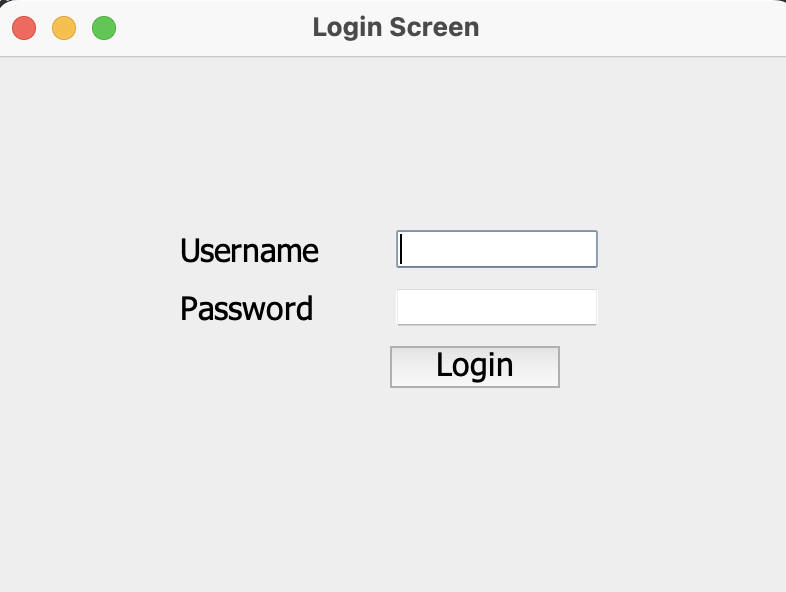
\includegraphics[width=0.5\textwidth]{assets/login-screen.png}
	\caption{Tampilan layar login}
	\label{fig:login-screen}
\end{figure}

\begin{figure}[h!]
	\centering
	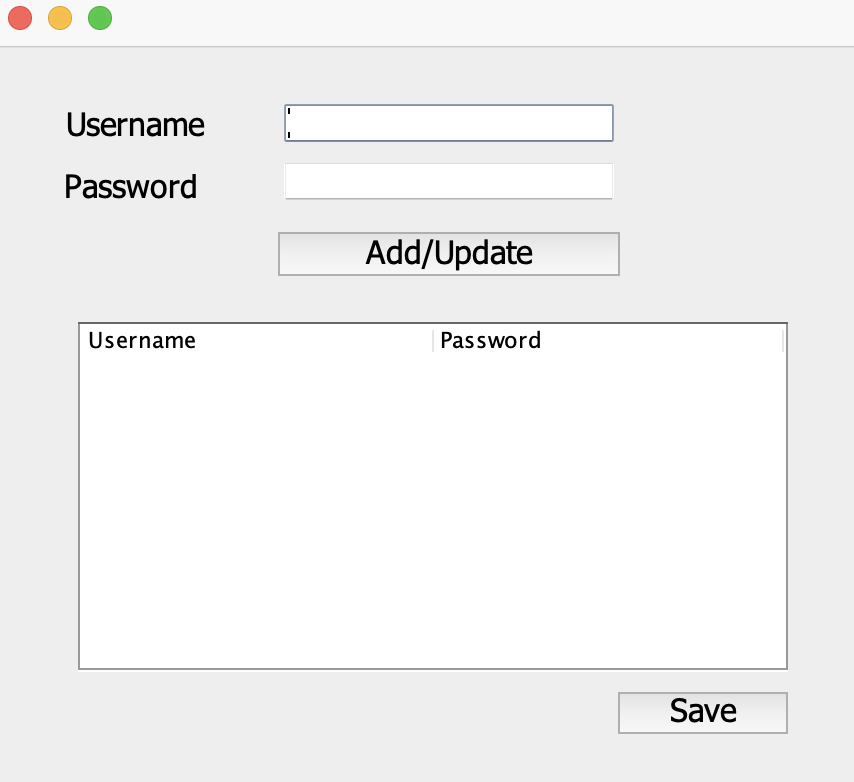
\includegraphics[width=0.5\textwidth]{assets/add-user-form.png}
	\caption{Tampilan formulir tambah pengguna}
	\label{fig:add-user-form}
\end{figure}

\textbf{Keterangan Gambar:} 
\begin{itemize}
	\item Gambar \ref{fig:login-screen}: Menampilkan tampilan GUI untuk login.
	\item Gambar \ref{fig:add-user-form}: Menampilkan tampilan GUI untuk menambah pengguna.
\end{itemize}



\section{Latihan dan Contoh Kode: Aplikasi Manajemen Buku}

\subsection{1. Kelas Book}

\begin{lstlisting}[style=JavaStyle]
	package edu.pradita.p10;
	
	public class Book {
		
		private String title;
		private String author;
		private int year;
		
		public Book(String title, String author, int year) {
			this.title = title;
			this.author = author;
			this.year = year;
		}
		
		public String getTitle() {
			return title;
		}
		
		public void setTitle(String title) {
			this.title = title;
		}
		
		public String getAuthor() {
			return author;
		}
		
		public void setAuthor(String author) {
			this.author = author;
		}
		
		public int getYear() {
			return year;
		}
		
		public void setYear(int year) {
			this.year = year;
		}
	}
\end{lstlisting}

\subsection{2. Kelas Data untuk Buku}

\begin{lstlisting}[style=JavaStyle]
	package edu.pradita.p10;
	
	import java.io.BufferedReader;
	import java.io.BufferedWriter;
	import java.io.File;
	import java.io.FileReader;
	import java.io.FileWriter;
	import java.io.IOException;
	import java.util.ArrayList;
	import java.util.List;
	
	public class Data {
		
		private static List<Book> books = new ArrayList<>();
		
		public static List<Book> getBooks() {
			return books;
		}
		
		public static List<Book> saveBooks(List<Book> books) {
			try {
				Data.books.clear();
				Data.books.addAll(books);
				
				File file = new File("books.csv");
				FileWriter fw = new FileWriter(file);
				BufferedWriter bw = new BufferedWriter(fw);
				
				for (Book book : Data.books) {
					bw.write(book.getTitle() + "," + book.getAuthor() + "," + book.getYear() + System.lineSeparator());
				}
				
				bw.close();
			} catch (IOException e) {
				e.printStackTrace();
			}
			
			return books;
		}
		
		public static List<Book> loadBooks() {
			try {
				File file = new File("books.csv");
				FileReader fr = new FileReader(file);
				BufferedReader br = new BufferedReader(fr);
				
				String line = br.readLine();
				while (line != null) {
					String[] lineArray = line.split(",");
					books.add(new Book(lineArray[0].trim(), lineArray[1].trim(), Integer.parseInt(lineArray[2].trim())));
					line = br.readLine();
				}
				br.close();
			} catch (IOException e) {
				e.printStackTrace();
			}
			
			return books;
		}
	}
\end{lstlisting}

\subsection{3. Kelas Formulir Buku}

\begin{lstlisting}[style=JavaStyle]
package edu.pradita.p10;

import java.awt.EventQueue;
import java.awt.Font;
import java.awt.GraphicsEnvironment;
import java.awt.event.ActionEvent;
import java.awt.event.ActionListener;
import java.util.ArrayList;
import java.util.List;

import javax.swing.JButton;
import javax.swing.JFrame;
import javax.swing.JLabel;
import javax.swing.JPanel;
import javax.swing.JScrollPane;
import javax.swing.JTable;
import javax.swing.JTextField;
import javax.swing.ListSelectionModel;
import javax.swing.border.EmptyBorder;
import javax.swing.event.ListSelectionEvent;
import javax.swing.event.ListSelectionListener;
import javax.swing.table.DefaultTableModel;

public class BookForm extends JFrame {
	
	/**
	* 
	*/
	private static final long serialVersionUID = 1L;
	private JPanel contentPane;
	private JTextField txtTitle;
	private JTable booksTable;
	private JTextField txtAuthor;
	private JTextField txtYear;
	private JButton btnSave;
	
	public static void main(String[] args) {
		EventQueue.invokeLater(new Runnable() {
			public void run() {
				try {
					BookForm frame = new BookForm();
					frame.setVisible(true);
				} catch (Exception e) {
					e.printStackTrace();
				}
			}
		});
	}
	
	public BookForm() {
		contentPane = new JPanel();
		contentPane.setBorder(new EmptyBorder(5, 5, 5, 5));
		setContentPane(contentPane);
		contentPane.setLayout(null);
		
		JLabel lblTitle = new JLabel("Title");
		lblTitle.setFont(new Font("Tahoma", Font.PLAIN, 16));
		lblTitle.setBounds(37, 33, 96, 13);
		contentPane.add(lblTitle);
		
		txtTitle = new JTextField();
		txtTitle.setFont(new Font("Tahoma", Font.PLAIN, 16));
		txtTitle.setBounds(143, 29, 171, 19);
		contentPane.add(txtTitle);
		txtTitle.setColumns(10);
		
		JLabel lblAuthor = new JLabel("Author");
		lblAuthor.setFont(new Font("Tahoma", Font.PLAIN, 16));
		lblAuthor.setBounds(36, 64, 75, 13);
		contentPane.add(lblAuthor);
		
		txtAuthor = new JTextField();
		txtAuthor.setFont(new Font("Tahoma", Font.PLAIN, 16));
		txtAuthor.setBounds(143, 60, 171, 19);
		contentPane.add(txtAuthor);
		txtAuthor.setColumns(10);
		
		JLabel lblYear = new JLabel("Year");
		lblYear.setFont(new Font("Tahoma", Font.PLAIN, 16));
		lblYear.setBounds(36, 95, 75, 13);
		contentPane.add(lblYear);
		
		txtYear = new JTextField();
		txtYear.setFont(new Font("Tahoma", Font.PLAIN, 16));
		txtYear.setBounds(143, 90, 171, 19);
		contentPane.add(txtYear);
		txtYear.setColumns(10);
		
		JButton btnAddUpdate = new JButton("Add/Update");
		btnAddUpdate.addActionListener(new ActionListener() {
			public void actionPerformed(ActionEvent e) {
				String title = txtTitle.getText().trim();
				String author = txtAuthor.getText().trim();
				int year = Integer.parseInt(txtYear.getText().trim());
				int rowCount = booksTable.getRowCount();
				DefaultTableModel table = (DefaultTableModel) booksTable.getModel();
				
				for (int i = 0; i <= table.getRowCount() - 1; i++) {
					if (title.equals(table.getValueAt(i, 0))) {
						table.setValueAt(author, i, 1);
						table.setValueAt(year, i, 2);
						return;
					}
				}
				table.insertRow(rowCount, new Object[] { title, author, year });
			}
		});
		btnAddUpdate.setFont(new Font("Tahoma", Font.PLAIN, 16));
		btnAddUpdate.setBounds(143, 123, 171, 22);
		contentPane.add(btnAddUpdate);
		
		JScrollPane scrollPane = new JScrollPane();
		scrollPane.setBounds(43, 158, 355, 175);
		contentPane.add(scrollPane);
		
		Object[][] data = new Object[Data.getBooks().size()][3];
		for (int i = 0; i < Data.getBooks().size(); i++) {
			Book book = Data.getBooks().get(i);
			data[i][0] = book.getTitle();
			data[i][1] = book.getAuthor();
			data[i][2] = book.getYear();
		}
		
		booksTable = new JTable();
		booksTable.setModel(new DefaultTableModel(data, new String[] { "Title", "Author", "Year" }) {
			/**
			* 
			*/
			private static final long serialVersionUID = 1L;
			Class[] columnTypes = new Class[] { String.class, String.class, Integer.class };
			
			public Class getColumnClass(int columnIndex) {
				return columnTypes[columnIndex];
			}
			
			boolean[] columnEditables = new boolean[] { false, false, false };
			
			public boolean isCellEditable(int row, int column) {
				return columnEditables[column];
			}
		});
		scrollPane.setViewportView(booksTable);
		booksTable.setSelectionMode(ListSelectionModel.SINGLE_SELECTION);
		booksTable.setFont(new Font("Tahoma", Font.PLAIN, 16));
		booksTable.getSelectionModel().addListSelectionListener(new ListSelectionListener() {
			@Override
			public void valueChanged(ListSelectionEvent e) {
				String title = booksTable.getValueAt(booksTable.getSelectedRow(), 0).toString();
				String author = booksTable.getValueAt(booksTable.getSelectedRow(), 1).toString();
				int year = (int) booksTable.getValueAt(booksTable.getSelectedRow(), 2);
				txtTitle.setText(title);
				txtAuthor.setText(author);
				txtYear.setText(String.valueOf(year));
			}
		});
		
		btnSave = new JButton("Save");
		btnSave.addActionListener(new ActionListener() {
			public void actionPerformed(ActionEvent e) {
				List<Book> books = new ArrayList<>();
				for (int i = 0; i < booksTable.getModel().getRowCount(); i++) {
					String title = booksTable.getValueAt(i, 0).toString(); 
					String author = booksTable.getValueAt(i, 1).toString(); 
					int year = Integer.parseInt(booksTable.getValueAt(i, 2).toString());
					books.add(new Book(title, author, year));
				}
				
				Data.saveBooks(books);
			}
		});
		btnSave.setFont(new Font("Tahoma", Font.PLAIN, 16));
		btnSave.setBounds(143, 346, 171, 22);
		contentPane.add(btnSave);
		
		this.setDefaultCloseOperation(JFrame.EXIT_ON_CLOSE);
		this.setBounds(centerX(500), centerY(450), 500, 450);
		this.setVisible(true);
	}
	
	private int centerX(int frameWidth) {
		return GraphicsEnvironment.getLocalGraphicsEnvironment().getCenterPoint().x - (frameWidth / 2);
	}
	
	private int centerY(int frameHeight) {
		return GraphicsEnvironment.getLocalGraphicsEnvironment().getCenterPoint().y - (frameHeight / 2);
	}
}
\end{lstlisting}

\begin{figure}[h!]
	\centering
	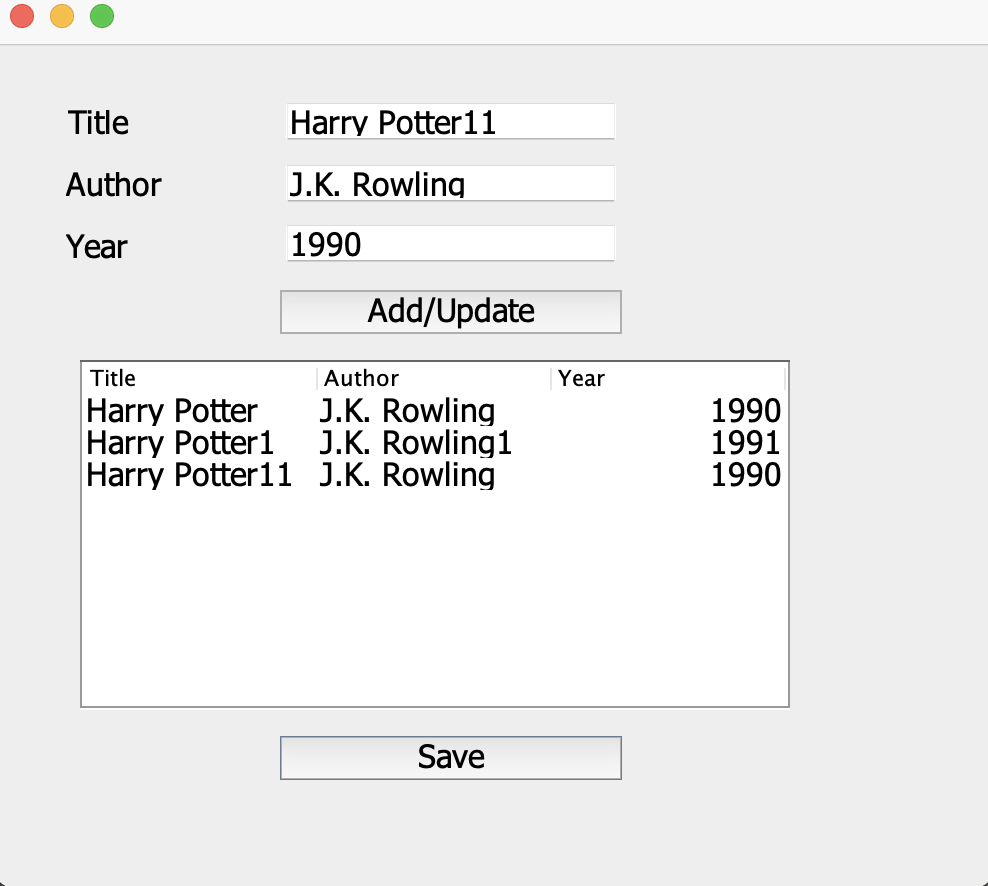
\includegraphics[width=0.5\textwidth]{assets/book-form.png}
	\caption{Tampilan layar book form}
\end{figure}



\section{Soal}

\subsection*{Soal 1: Aplikasi Manajemen Karyawan}

\textbf{Konteks dan Kasus:} \\
Anda diminta untuk membuat aplikasi manajemen karyawan di sebuah perusahaan. Setiap karyawan memiliki nama, jabatan, dan gaji. Aplikasi ini memungkinkan pengguna untuk menambahkan karyawan baru, mengedit informasi karyawan yang sudah ada, dan menyimpan data karyawan ke dalam file CSV.

\textbf{Tugas:}
\begin{enumerate}
	\item Buat kelas \texttt{Employee} yang memiliki atribut \texttt{name}, \texttt{position}, dan \texttt{salary}.
	\item Implementasikan kelas \texttt{EmployeeData} untuk memanage data karyawan termasuk menyimpan dan memuat data ke/dari file CSV.
	\item Implementasikan GUI untuk mengelola data karyawan dalam aplikasi.
	\item Tambahkan fitur untuk menghitung total gaji semua karyawan dan menampilkannya di dalam GUI.
\end{enumerate}

\subsection*{Soal 2: Aplikasi Pengelolaan Inventori Barang}

\textbf{Konteks dan Kasus:} \\
Sebuah toko retail ingin membuat aplikasi untuk mengelola inventori barang. Setiap barang memiliki nama, kategori, dan jumlah stok. Aplikasi ini memungkinkan pengguna untuk menambahkan barang baru, mengedit informasi barang yang ada, dan menyimpan data barang ke dalam file CSV.

\textbf{Tugas:}
\begin{enumerate}
	\item Buat kelas \texttt{Product} yang memiliki atribut \texttt{name}, \texttt{category}, dan \texttt{quantity}.
	\item Implementasikan kelas \texttt{InventoryData} untuk mengelola data barang termasuk menyimpan dan memuat data ke/dari file CSV.
	\item Implementasikan GUI untuk mengelola data barang dalam aplikasi.
	\item Tambahkan fitur untuk memantau stok barang, dengan memberikan peringatan jika stok barang tertentu kurang dari jumlah minimum yang ditentukan.
\end{enumerate}
	\chapter{Graphical User Interface}


\section{Pengenalan GUI di Java}

\subsection{Pengantar GUI di Java}
Graphical User Interface (GUI) di Java digunakan untuk membuat antarmuka pengguna yang interaktif dengan elemen-elemen visual seperti tombol, teks, label, dan lain-lain. Java menyediakan beberapa toolkit untuk membuat GUI, salah satunya adalah Swing, yang sangat populer digunakan.

Swing adalah bagian dari Java Foundation Classes (JFC) yang menyediakan alat dan komponen untuk membuat aplikasi desktop yang interaktif. Kelas utama dalam Swing meliputi \texttt{JFrame}, \texttt{JPanel}, \texttt{JLabel}, \texttt{JButton}, dan banyak lagi.

\subsection{Instalasi WindowBuilder di Eclipse}

\begin{enumerate}
	\item Buka Eclipse IDE.
	\item Pilih menu \texttt{Help} > \texttt{Install New Software}.
	\item Pada kotak \texttt{Work with}, pilih URL sesuai dengan versi eclipse yang kalian miliki
	\item Tekan \texttt{Enter}, dan Eclipse akan memuat daftar software yang tersedia dari URL tersebut.
	\item Centang opsi \texttt{WindowBuilder Swing Designer}, lalu klik \texttt{Next}.
	\item Ikuti petunjuk instalasi yang diberikan hingga selesai.
	\item Setelah instalasi selesai, restart Eclipse.
	\item WindowBuilder kini siap digunakan untuk membuat aplikasi GUI di Java.
\end{enumerate}


\subsection{Membuat GUI dengan WindowBuilder}

Setelah WindowBuilder diinstal, Anda bisa mulai membuat aplikasi GUI di Java dengan lebih mudah. WindowBuilder menyediakan editor drag-and-drop untuk menambahkan komponen GUI seperti tombol, label, dan panel tanpa perlu menulis kode secara manual.

Langkah-langkah membuat GUI menggunakan WindowBuilder:
\begin{enumerate}
	\item Buat project Java baru di Eclipse.
	\item Klik kanan pada package, pilih \texttt{New} > \texttt{Other}.
	\item Pilih \texttt{WindowBuilder} > \texttt{Swing Designer} > \texttt{JFrame}, lalu klik \texttt{Next}.
	\item Beri nama kelas dan klik \texttt{Finish}.
	\item Anda akan melihat editor GUI, di mana Anda dapat mendesain antarmuka dengan drag-and-drop komponen dari palet ke form.
	\item Tambahkan komponen yang diperlukan, seperti \texttt{JButton}, \texttt{JLabel}, \texttt{JTextField}, dll.
	\item Setelah selesai, simpan dan jalankan program untuk melihat GUI yang telah dibuat.
\end{enumerate}



\subsection{Opsional: Error pada WindowBuilder}

Jika terjadi error saat penggunaan WindowBuilder, ikuti langkah berikut:

\begin{enumerate}
	\item Buka Eclipse IDE.
	\item Pilih menu \texttt{Eclipse} > \texttt{Settings}.
	\item Pilih bagian \texttt{ Install/Update}, lalu pilih  \texttt{Available Software Sites}
	\item Uncheck bagian \texttt{Latest Eclipse IDE Packages Release} dan  \texttt{Latest Eclipse Simultaneaous Release}
	\item Klik \texttt{Apply and Close}
\end{enumerate}



	
\section{Contoh Kode dan Penjelasan}

\subsection{Kalkulator GUI}

\textbf{Kode:} \texttt{Calculator.java}

\textbf{Deskripsi:} Kode ini membuat aplikasi kalkulator sederhana menggunakan Swing di Java. Program ini terdiri dari beberapa komponen GUI seperti tombol angka, tombol operasi, dan layar tampilan.

\textbf{Penjelasan Kode:}
\begin{itemize}
	\item \texttt{Calculator} adalah kelas utama yang memperluas \texttt{JFrame} untuk membuat jendela GUI.
	\item \texttt{JPanel} digunakan untuk menyusun komponen dengan layout \texttt{BorderLayout} dan \texttt{GridLayout}.
	\item \texttt{JLabel} digunakan untuk menampilkan hasil kalkulasi.
	\item Tombol angka dibuat secara dinamis dalam sebuah loop dan ditambahkan ke panel tombol.
	\item Tombol \texttt{+} dan \texttt{=} ditambahkan untuk melakukan operasi penjumlahan dan menampilkan hasil.
	\item \texttt{calculate()} adalah metode untuk menghitung hasil operasi berdasarkan nilai yang disimpan dalam \texttt{accumulator}.
\end{itemize}

\textbf{Gambar:} \\
\begin{center}
	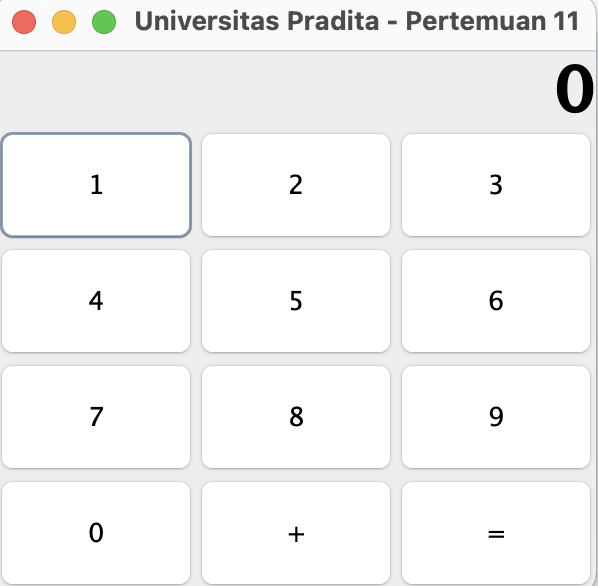
\includegraphics[width=0.5\textwidth]{assets/pertemuan11/calculator.png}
\end{center}

\textbf{Kode Java:}
\begin{lstlisting}[style=JavaStyle]
	package edu.pradita.p11;
	
	import java.awt.BorderLayout;
	import java.awt.Font;
	import java.awt.GridLayout;
	import java.awt.event.ActionEvent;
	import java.awt.event.ActionListener;
	import javax.swing.JButton;
	import javax.swing.JFrame;
	import javax.swing.JLabel;
	import javax.swing.JPanel;
	
	public class Calculator extends JFrame {
		
		private static final int FRAME_WIDTH = 300;
		private static final int FRAME_HEIGHT = 300;
		private static final int FONT_SIZE = 32;
		
		private Integer accumulator = null;
		private Integer value = 0;
		private String nextOperation = null;
		private boolean clearDisplay = false;
		
		public Calculator() {
			JPanel mainPanel = new JPanel();
			mainPanel.setLayout(new BorderLayout());
			this.add(mainPanel);
			
			JLabel display = new JLabel();
			display.setHorizontalAlignment(JLabel.RIGHT);
			display.setFont(new Font(display.getFont().getName(), Font.BOLD, 32));
			display.setText(String.valueOf(value));
			mainPanel.add(display, BorderLayout.NORTH);
			
			JPanel buttonPanel = new JPanel();
			buttonPanel.setLayout(new GridLayout(4, 3));
			mainPanel.add(buttonPanel, BorderLayout.CENTER);
			
			// Loop adding numeric button
			for (int i = 1; i <= 10; i++) {
				String valueText = (i < 10) ? valueText = String.valueOf(i) : "0";
				JButton button = new JButton();
				button.setText(valueText);
				buttonPanel.add(button);
				
				ActionListener numericButtonListener = new ActionListener() {
					@Override
					public void actionPerformed(ActionEvent e) {
						if (display.getText().equals("0")) {
							display.setText("" + button.getText());
						} else {
							if (clearDisplay) {
								display.setText("");
								clearDisplay = false;
							}
							display.setText(display.getText() + button.getText());
						}
						value = Integer.valueOf(display.getText());
					}
				};
				button.addActionListener(numericButtonListener);
			}
			
			// adding add button
			JButton button = new JButton();
			button.setText("+");
			buttonPanel.add(button);
			
			ActionListener addButtonListener = new ActionListener() {
				@Override
				public void actionPerformed(ActionEvent e) {
					nextOperation = "+";
					if (accumulator == null) {
						accumulator = Integer.valueOf(display.getText());
					} else {
						calculate();
						display.setText(String.valueOf(accumulator));
					}
					value = 0;
					clearDisplay = true;
				}
			};
			button.addActionListener(addButtonListener);
			
			// adding equal button
			JButton equalButton = new JButton();
			equalButton.setText("=");
			buttonPanel.add(equalButton);
			
			ActionListener equalButtonListener = new ActionListener() {
				@Override
				public void actionPerformed(ActionEvent e) {
					if (accumulator != null && nextOperation != null) {
						calculate();
						display.setText(String.valueOf(accumulator));
					}
					clearDisplay = true;
				}
			};
			equalButton.addActionListener(equalButtonListener);
			
			setSize(FRAME_WIDTH, FRAME_HEIGHT);
		}
		
		public void calculate() {
			if (nextOperation == "+") {
				accumulator = accumulator + value;
			}
		}
	}
\end{lstlisting}



\subsection{Form dengan WindowBuilder}

\textbf{Kode:} \texttt{MyForm.java}

\textbf{Deskripsi:} Kode ini menciptakan formulir dengan beberapa komponen Swing, termasuk \texttt{JTextField}, \texttt{JSpinner}, dan \texttt{JButton}. Program ini juga menambahkan tombol yang memungkinkan pengguna untuk menambahkan tombol lain ke dalam formulir secara dinamis.

\textbf{Penjelasan Kode:}
\begin{itemize}
	\item \texttt{MyForm} adalah kelas yang membuat formulir dengan komponen GUI.
	\item \texttt{JTextField} digunakan untuk memasukkan teks, dan \texttt{JSpinner} untuk memilih nilai numerik.
	\item \texttt{JButton} digunakan untuk menyimpan data dan menambahkan tombol tambahan ke formulir.
	\item Metode \texttt{initialize()} mengatur layout dan menambahkan komponen ke formulir.
\end{itemize}

\textbf{Gambar:} \\
\begin{center}
	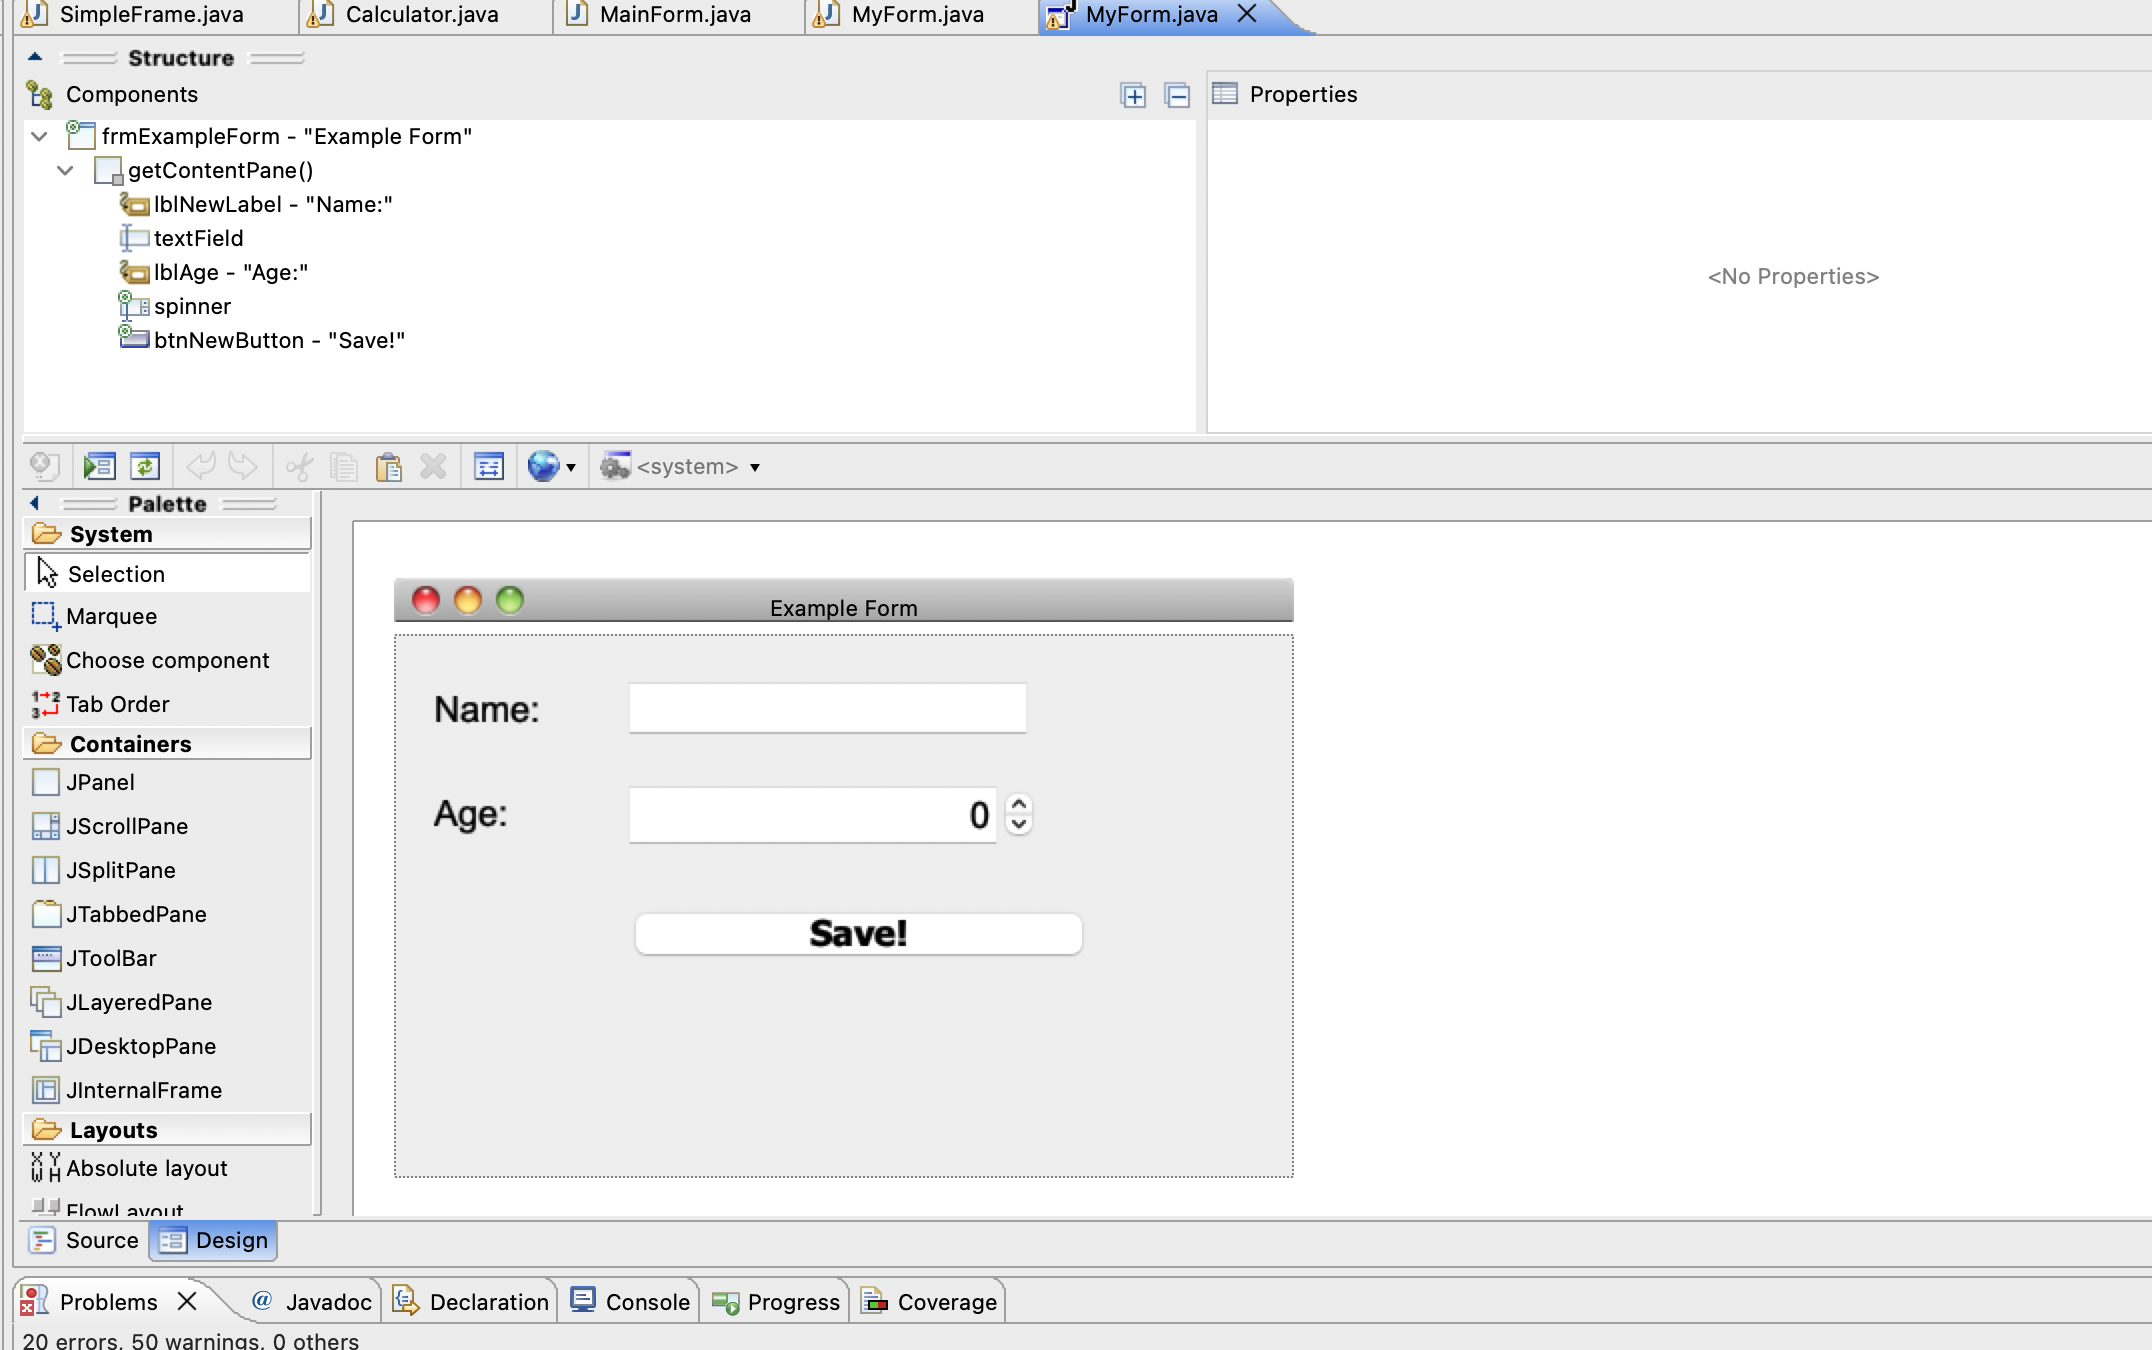
\includegraphics[width=0.8\textwidth]{assets/pertemuan11/myform_window_builder.png}
	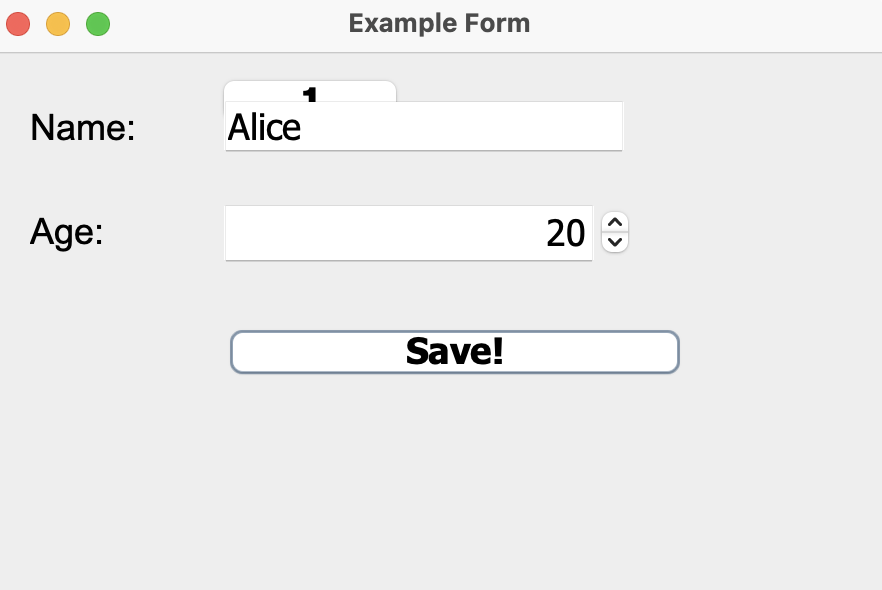
\includegraphics[width=0.8\textwidth]{assets/pertemuan11/myform.png}
	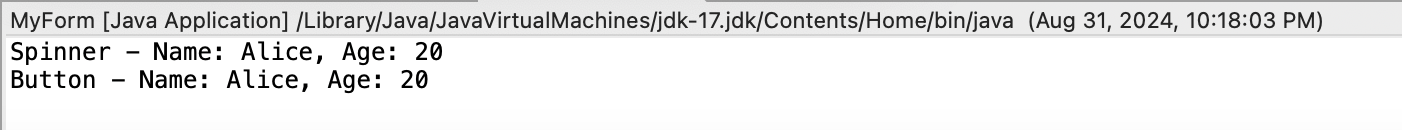
\includegraphics[width=0.8\textwidth]{assets/pertemuan11/myform_result.png}
\end{center}

\textbf{Kode Java:}
\begin{lstlisting}[style=JavaStyle]
	package edu.pradita.p11;
	
	import java.awt.EventQueue;
	import java.awt.Font;
	import java.awt.event.ActionEvent;
	import java.awt.event.ActionListener;
	import javax.swing.JButton;
	import javax.swing.JFrame;
	import javax.swing.JLabel;
	import javax.swing.JPanel;
	import javax.swing.JTextField;
	import javax.swing.JSpinner;
	import javax.swing.SpinnerNumberModel;
	
	public class MyForm extends JFrame {
		
		private JTextField nameField;
		private JSpinner ageSpinner;
		private JButton addButton;
		private JPanel panel;
		
		public MyForm() {
			initialize();
		}
		
		private void initialize() {
			setTitle("My Form");
			setBounds(100, 100, 450, 300);
			setDefaultCloseOperation(JFrame.EXIT_ON_CLOSE);
			panel = new JPanel();
			getContentPane().add(panel);
			panel.setLayout(null);
			
			JLabel nameLabel = new JLabel("Name:");
			nameLabel.setFont(new Font("Arial", Font.PLAIN, 14));
			nameLabel.setBounds(10, 20, 80, 25);
			panel.add(nameLabel);
			
			nameField = new JTextField();
			nameField.setBounds(100, 20, 165, 25);
			panel.add(nameField);
			
			JLabel ageLabel = new JLabel("Age:");
			ageLabel.setFont(new Font("Arial", Font.PLAIN, 14));
			ageLabel.setBounds(10, 50, 80, 25);
			panel.add(ageLabel);
			
			ageSpinner = new JSpinner(new SpinnerNumberModel(18, 0, 100, 1));
			ageSpinner.setBounds(100, 50, 50, 25);
			panel.add(ageSpinner);
			
			addButton = new JButton("Add");
			addButton.setBounds(10, 80, 80, 25);
			panel.add(addButton);
			
			addButton.addActionListener(new ActionListener() {
				@Override
				public void actionPerformed(ActionEvent e) {
					// Add action handling code here
				}
			});
			
			JButton addDynamicButton = new JButton("Add Dynamic Button");
			addDynamicButton.setBounds(10, 110, 200, 25);
			panel.add(addDynamicButton);
			
			addDynamicButton.addActionListener(new ActionListener() {
				@Override
				public void actionPerformed(ActionEvent e) {
					JButton dynamicButton = new JButton("Dynamic Button");
					dynamicButton.setBounds(10, 140 + (panel.getComponentCount() - 6) * 30, 200, 25);
					panel.add(dynamicButton);
					panel.revalidate();
					panel.repaint();
				}
			});
		}
		
		public static void main(String[] args) {
			EventQueue.invokeLater(new Runnable() {
				public void run() {
					try {
						MyForm frame = new MyForm();
						frame.setVisible(true);
					} catch (Exception e) {
						e.printStackTrace();
					}
				}
			});
		}
	}
\end{lstlisting}

\subsection{Frame Sederhana}

\textbf{Kode:} \texttt{SimpleFrame.java}

\textbf{Deskripsi:} Kode ini membuat jendela GUI sederhana dengan \texttt{JTextField}, \texttt{JButton}, dan \texttt{JLabel}. Ketika tombol diklik, label akan diperbarui untuk menampilkan pesan yang menyapa pengguna dengan nama yang dimasukkan.

\textbf{Penjelasan Kode:}
\begin{itemize}
	\item \texttt{SimpleFrame} adalah kelas yang memperluas \texttt{JFrame} untuk membuat jendela GUI.
	\item \texttt{JTextField} digunakan untuk memasukkan nama.
	\item \texttt{JButton} ketika diklik, akan memperbarui \texttt{JLabel} dengan pesan yang menyapa pengguna.
	\item Kode ini juga mengatur ukuran frame dengan \texttt{setSize}.
\end{itemize}

\textbf{Gambar:} \\
\begin{center}
	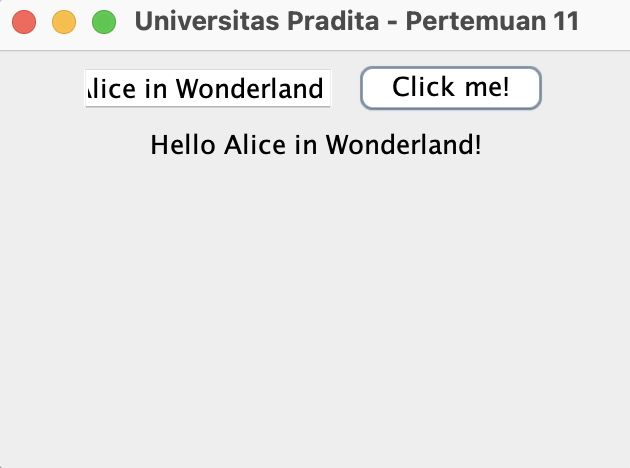
\includegraphics[width=0.8\textwidth]{assets/pertemuan11/simple_frame.png}
\end{center}


\textbf{Kode Java:}
\begin{lstlisting}[style=JavaStyle]
	package edu.pradita.p11;
	
	import java.awt.event.ActionEvent;
	import java.awt.event.ActionListener;
	import javax.swing.JButton;
	import javax.swing.JFrame;
	import javax.swing.JLabel;
	import javax.swing.JPanel;
	import javax.swing.JTextField;
	
	public class SimpleFrame extends JFrame {
		
		private JTextField textField;
		private JLabel label;
		
		public SimpleFrame() {
			setTitle("Simple Frame");
			setSize(300, 200);
			setDefaultCloseOperation(JFrame.EXIT_ON_CLOSE);
			setLocationRelativeTo(null);
			
			JPanel panel = new JPanel();
			getContentPane().add(panel);
			panel.setLayout(null);
			
			JLabel promptLabel = new JLabel("Enter your name:");
			promptLabel.setBounds(10, 20, 150, 25);
			panel.add(promptLabel);
			
			textField = new JTextField();
			textField.setBounds(10, 50, 160, 25);
			panel.add(textField);
			
			JButton button = new JButton("Say Hello");
			button.setBounds(10, 80, 160, 25);
			panel.add(button);
			
			label = new JLabel();
			label.setBounds(10, 110, 250, 25);
			panel.add(label);
			
			button.addActionListener(new ActionListener() {
				@Override
				public void actionPerformed(ActionEvent e) {
					String name = textField.getText();
					label.setText("Hello, " + name + "!");
				}
			});
		}
		
		public static void main(String[] args) {
			SimpleFrame frame = new SimpleFrame();
			frame.setVisible(true);
		}
	}
\end{lstlisting}



\subsection{Main Form}

\textbf{Kode:} \texttt{MainForm.java}

\textbf{Deskripsi:} Kode ini membuat dua jendela GUI: satu untuk \texttt{SimpleFrame} dan satu untuk \texttt{Calculator}. \texttt{MainForm} adalah kelas utama yang menjalankan aplikasi dan menampilkan kedua jendela.

\textbf{Penjelasan Kode:}
\begin{itemize}
	\item \texttt{MainForm} adalah kelas utama dengan metode \texttt{main} yang membuat dan menampilkan jendela \texttt{SimpleFrame} dan \texttt{Calculator}.
	\item \texttt{frame.setLocationRelativeTo(null)} memastikan jendela ditempatkan di pusat layar.
	\item \texttt{setTitle}, \texttt{setDefaultCloseOperation}, dan \texttt{setVisible} digunakan untuk mengatur judul, operasi penutupan, dan visibilitas jendela.
\end{itemize}

\textbf{Gambar:} \\
\begin{center}
	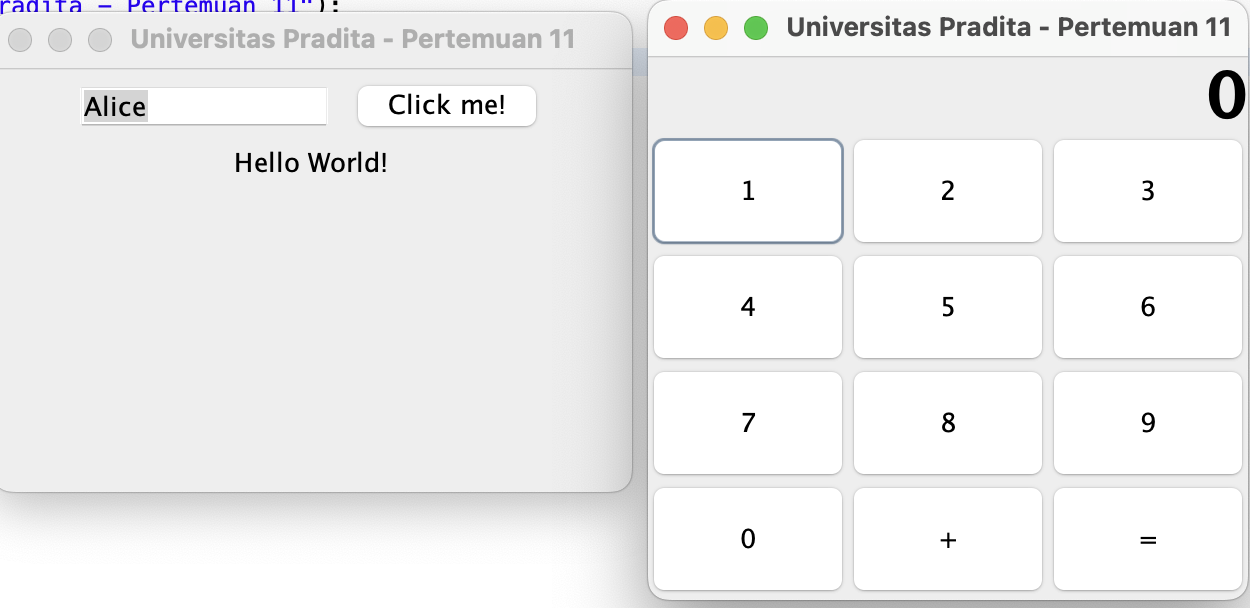
\includegraphics[width=0.8\textwidth]{assets/pertemuan11/main_form.png}
\end{center}

\textbf{Kode Java:}
\begin{lstlisting}[style=JavaStyle]
	package edu.pradita.p11;
	
	import javax.swing.JFrame;
	
	public class MainForm {
		public static void main(String[] args) {
			JFrame frame = new SimpleFrame();
			frame.setLocationRelativeTo(null); // put the frame at the centre
			frame.setTitle("Universitas Pradita - Pertemuan 11");
			frame.setDefaultCloseOperation(JFrame.EXIT_ON_CLOSE);
			frame.setVisible(true);
			
			JFrame calculator = new Calculator();
			calculator.setLocationRelativeTo(null); // put the frame at the centre
			calculator.setTitle("Universitas Pradita - Pertemuan 11");
			calculator.setDefaultCloseOperation(JFrame.EXIT_ON_CLOSE);
			calculator.setVisible(true);
		}
	}
\end{lstlisting}


\section{Latihan dan Contoh Kode: BMI Calculator}

Pada latihan ini, Anda akan membuat aplikasi GUI untuk menghitung Body Mass Index (BMI). Aplikasi ini harus memiliki inputan untuk berat badan (dalam kilogram) dan tinggi badan (dalam meter). Setelah pengguna memasukkan data dan menekan tombol “Hitung”, BMI akan ditampilkan di layar.

\textbf{Instruksi:}
\begin{enumerate}
	\item Buatlah GUI menggunakan WindowBuilder di Eclipse.
	\item Buatlah inputan untuk berat badan (dalam kilogram) dan tinggi badan (dalam meter).
	\item Tambahkan tombol “Hitung” yang akan menghitung BMI berdasarkan inputan pengguna.
	\item Tampilkan hasil BMI setelah tombol ditekan.
\end{enumerate}


\textbf{Gambar:} \\
\begin{center}
	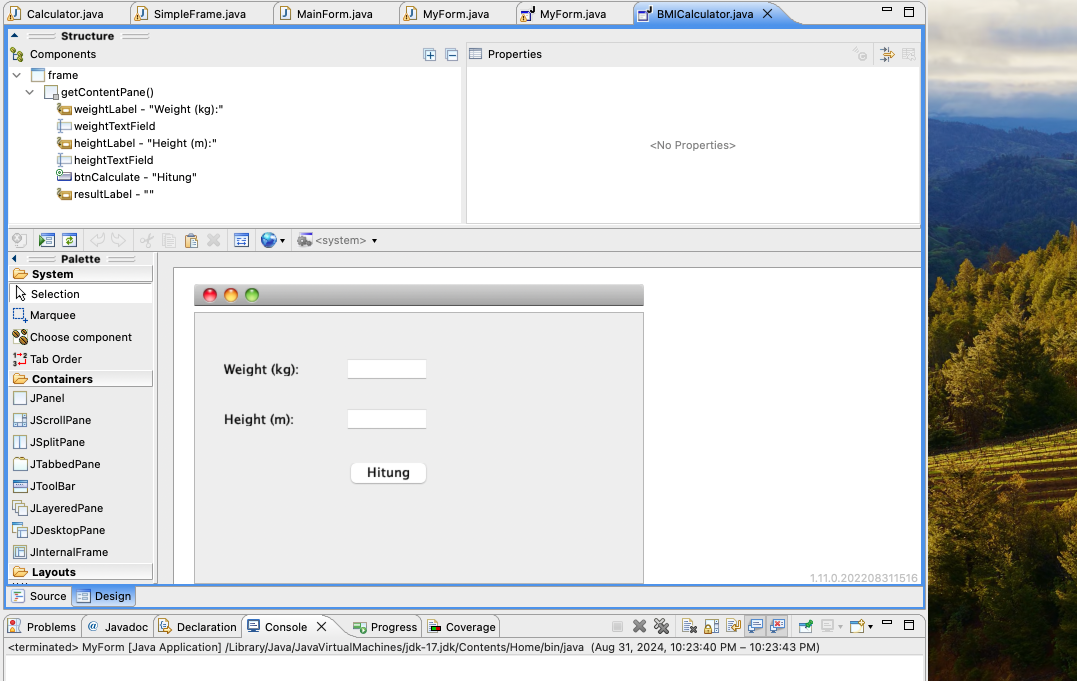
\includegraphics[width=0.8\textwidth]{assets/pertemuan11/bmicalculator_window_builder.png}
	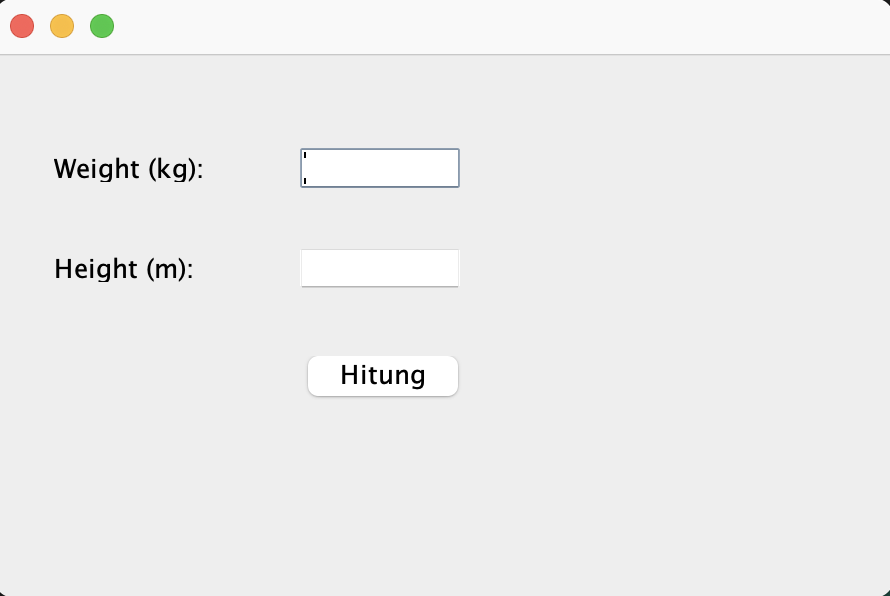
\includegraphics[width=0.8\textwidth]{assets/pertemuan11/bmicalculator.png}
\end{center}


\textbf{Kode Java:}

\begin{lstlisting}[style=JavaStyle]
	import java.awt.EventQueue;
	import javax.swing.JFrame;
	import javax.swing.JLabel;
	import javax.swing.JTextField;
	import javax.swing.JButton;
	import java.awt.event.ActionListener;
	import java.awt.event.ActionEvent;
	
	public class BMICalculator {
		
		private JFrame frame;
		private JTextField weightTextField;
		private JTextField heightTextField;
		private JLabel resultLabel;
		
		/**
		* Launch the application.
		*/
		public static void main(String[] args) {
			EventQueue.invokeLater(new Runnable() {
				public void run() {
					try {
						BMICalculator window = new BMICalculator();
						window.frame.setVisible(true);
					} catch (Exception e) {
						e.printStackTrace();
					}
				}
			});
		}
		
		/**
		* Create the application.
		*/
		public BMICalculator() {
			initialize();
		}
		
		/**
		* Initialize the contents of the frame.
		*/
		private void initialize() {
			frame = new JFrame();
			frame.setBounds(100, 100, 450, 300);
			frame.setDefaultCloseOperation(JFrame.EXIT_ON_CLOSE);
			frame.getContentPane().setLayout(null);
			
			JLabel weightLabel = new JLabel("Weight (kg):");
			weightLabel.setBounds(30, 50, 100, 14);
			frame.getContentPane().add(weightLabel);
			
			weightTextField = new JTextField();
			weightTextField.setBounds(150, 47, 86, 20);
			frame.getContentPane().add(weightTextField);
			weightTextField.setColumns(10);
			
			JLabel heightLabel = new JLabel("Height (m):");
			heightLabel.setBounds(30, 100, 100, 14);
			frame.getContentPane().add(heightLabel);
			
			heightTextField = new JTextField();
			heightTextField.setBounds(150, 97, 86, 20);
			frame.getContentPane().add(heightTextField);
			heightTextField.setColumns(10);
			
			JButton btnCalculate = new JButton("Hitung");
			btnCalculate.addActionListener(new ActionListener() {
				public void actionPerformed(ActionEvent e) {
					double weight = Double.parseDouble(weightTextField.getText());
					double height = Double.parseDouble(heightTextField.getText());
					double bmi = weight / (height * height);
					resultLabel.setText(String.format("Your BMI is: %.2f", bmi));
				}
			});
			btnCalculate.setBounds(150, 150, 89, 23);
			frame.getContentPane().add(btnCalculate);
			
			resultLabel = new JLabel("");
			resultLabel.setBounds(150, 200, 200, 14);
			frame.getContentPane().add(resultLabel);
		}
	}
\end{lstlisting}


\section{Soal}

\subsection{Aplikasi Manajemen Tugas}

Pada latihan ini, Anda akan membuat aplikasi manajemen tugas sederhana yang memungkinkan pengguna untuk menambahkan, melihat, dan menghapus tugas. Aplikasi ini harus memiliki antarmuka GUI yang memungkinkan pengguna untuk mengelola daftar tugas dengan mudah. Setiap tugas terdiri dari nama tugas, deskripsi, dan status (selesai atau belum selesai).

Instruksi: 
\begin{enumerate} 
	\item Buatlah GUI menggunakan \texttt{WindowBuilder} di Eclipse. 
	\item Tambahkan inputan untuk memasukkan nama tugas dan deskripsi tugas. 
	\item Tambahkan checkbox untuk menandai apakah tugas sudah selesai atau belum. 
	\item Implementasikan fitur untuk menambahkan tugas baru ke dalam daftar tugas. 
	\item Tambahkan daftar tugas yang dapat menampilkan semua tugas yang telah ditambahkan.
\end{enumerate}

		
\end{document}
